\documentclass[12pt]{My_preprint}
\usetikzlibrary{arrows.meta,
                chains,
                positioning,
                shapes.geometric}

%%%%%%%%%%%%%%%%%%%%%%%%%%%%%%%%%%%%%%%%%%%%%%%%%%%%%%%%%%%%%%%%%%%%%%%%%%%%%%%
\newcommand{\size}{0.22\textwidth}
\newcommand{\avg}[1]{\left<#1\right>}
\renewcommand{\avg}[1]{\left<#1\right>}
\newcommand{\condavg}[1]{\left<#1 | \mathscr{C}_1\right>}
\newcommand{\Exp}[1]{\overline{\overline{#1}}}
\newcommand{\davg}[1]{\left<#1\right>_d}
\newcommand{\cavg}[1]{\left<#1\right>_c}
\newcommand{\pavg}[1]{\avg{\delta_\alpha #1}}
% \newcommand{\pnavg}[1]{n\left<#1\right>_p}

\newcommand{\avgcond}[1]{\left<#1\right>}
\renewcommand{\avgcond}[1]{\overline{#1}}
\newcommand{\kavg}[1]{\avgcond{#1}^k}
\newcommand{\Iavg}[1]{\avgcond{#1}^I}
\newcommand{\pnnavg}[1]{\avgcond{#1}^{p}}
\newcommand{\pnavg}[1]{n_p\pnnavg{#1}}
\newcommand{\oneavg}[1]{\avgcond{#1}^1}
\newcommand{\twoavg}[1]{\avgcond{#1}^2}
\newcommand{\smallavg}[2]{\avgcond{#1}^{#2}}
\newcommand{\sym}[1]{\text{Sym}\left[#1\right]}

\newcommand{\nstavg}[1]{\overline{#1}_{nst}}
\newcommand{\nstrelavg}[1]{\overline{#1}_{nst}^{rel}}
\newcommand{\mavg}[1]{\left<#1\right>_m}
\newcommand{\gavg}[2][\gamma]{\left<#2\right>_{#1}}
\newcommand{\partials}[1]{\partial_{i_1}\partial_{i_2}\ldots\partial{i_{#1}}}
\newcommand{\partialp}[2]{ \prod_{m=#1}^{#2} \partial_{i_m}}
\newcommand{\hatpartialp}[2]{ \prod_{m=#1}^{#2} \hat{\partial}_{j_m}}
\newcommand{\hatpartialpi}[2]{ \prod_{m=#1}^{#2} \hat{\partial}_{i_m}}
\newcommand{\pri}[2]{ \prod_{m=#1}^{#2} r_{i_m}}
\newcommand{\prj}[2]{ \prod_{m=#1}^{#2} r_{j_m}}

\newcommand{\grad}{\mathbf{\nabla}}
\renewcommand{\div}{\mathbf{\nabla}\cdot}
\newcommand{\gradI}{\mathbf{\nabla}_{||}}
\newcommand{\divI}{\mathbf{\nabla}_{||}\cdot}

\newcommand{\ddt}{\frac{d}{d t}}
\newcommand{\pddt}{\frac{\partial}{\partial t}}
\renewcommand{\pddt}{\partial_t}
\newcommand{\norm}[1]{\hat{#1}}
\newcommand{\Jump}[1]{\llbracket #1 \rrbracket \cdot \textbf{n} }

%%% Utiliser pour les commentaires
\newcommand{\JL}[1]{\color{red}#1\color{black}}
\newcommand{\DL}[1]{\color{green}#1\color{black}}
\newcommand{\tb}[1]{\color{blue}#1\color{black}}
% \renewcommand{\alpha}{}
\renewcommand{\JL}[1]{}
% \renewcommand{\tb}[1]{}

\renewcommand{\size}[1]{0.3\textwidth}
\newcommand{\expo}[2][n]{\frac{(-1)^#1}{#1!} \partialp{1}{#1} \pavg{\int_{\Omega_\alpha} \pri{1}{#1}#2 d\Omega}}
\newcommand{\expoU}[2][n]{\frac{(-1)^#1}{#1!} \partialp{1}{#1} \pavg{\textbf{u}_\alpha\int_{\Omega_\alpha} \pri{1}{#1}#2 d\Omega}}
\newcommand{\expoS}[2][n]{\frac{(-1)^#1}{#1!} \partialp{1}{#1} \pavg{\int_{\Sigma_\alpha} \pri{1}{#1}#2 d\Sigma}}

% \newcommand{\numref}[1]{\ref{#1}}
\renewcommand{\ref}[1]{\autoref{#1}}

%%%%%%%%%%%%%%%%%%%%%%%%%%%%%%% Title & Author %%%%%%%%%%%%%%%%%%%%%%%%%%%%%%%%


%\title{The hybrid model for arbitrary dispersed multiphase flows with surface properties}
\title{Averaged equations for disperse two-phase flow made of fluid particles}

\author[1,2]{Nicolas Fintzi}
\author[1]{Jean-Lou Pierson}
% \author[2]{Stephane Popinet}
\author[2]{Daniel Lhuillier}
\affil[1]{IFP Energies Nouvelles, Rond-point de l’changeur de Solaize, 69360 Solaize}
\affil[2]{Sorbonne Université, Institut Jean le Rond ∂’Alembert, 4 place Jussieu, 75252 PARIS CEDEX 05, France}

\begin{document}

\maketitle

\begin{abstract}
    This article presents a comprehensive study of the averaged equations for dispersed multiphase flows.
    We present a systematic derivation of a general averaged hybrid model that incorporates the influence of surface properties of fluid particles dispersed in a continuous phase.
    The dispersed phase averaged equations are derived using two distinct formalism :
    the particle-average or Lagrangian formalism proposed by \citet{zhang1994ensemble,jackson1997locally};
    and the phase-average method, which is also employed for the continuous phase based on the approach of \citet{drew1983mathematical}. 
    The particle-phase averaged formalism yields the conventional linear conservation equations, as well as the less familiar moments' conservation equations.
    The primary contribution of this work is the global derivation of these equations in their most generalized form.
    The second contribution is the demonstration of the equivalence between the particle-averaged and phase-averaged equations. 
    We show that the phase-averaged equation of the dispersed phase, is in fact a series expansion of the so-called particle-averaged moments equations. 
    % Consequently, as first stated by \citet{zhang1997momentum} and \citet{lhuillier2000bilan}, we proved that by incorporating an arbitrary number of moment equations, we can achieve an arbitrary order of accuracy in the modeling of the dispersed phase.
    Finally, to provide a practical application and enhance the understanding of the first-moments conservation laws, we propose to study various examples.
    In particular, we demonstrate how to derive a hybrid model capable to predict the distribution of surfactant over the interface of bubbles in contaminated rising bubbly flows.
\end{abstract}
\listoftodos
\todo[inline]{add exponant for microscopic quantities}
\tb{point out the non equivalence when there is mass transfer or so }

\tb{give a rigourous expression for the first moment }

\JL{Je ne trouve pas le titre tres parlant : the hybrid model parle peu pour des non specialistes et qu'entends tu par surface properties ? j'ai modifie, mais cela pourra sans doute changer encore.}


\section{Introduction}

Dispersed multiphase flows are ubiquitous in numerous engineering and scientific domains. 
Examples include gas-solid flows in fluidized bed reactors, oil-water emulsions in petroleum industry processes, and fiber suspension in composite manufacturing. 
Developing a versatile model capable of capturing the various nature of the dispersed multiphase flow is therefore essential.
In this work we aim to bridge the existing gaps in current models by providing a unified and adaptable framework for any kind of dispersed multiphase flow problems.

Numerous example of dispersed two-phase flows model have been proposed this last two decades.
As started by \citep{zhang1994averaged,zhang1994ensemble} where they study spherical bubbles suspension.
They provided closures in the inviscid flow limit for the mass and momentum transport equation. 
After that \citet{jackson1997locally,zhang1997momentum} derive the averaged conservation equations for a solid spherical particle suspension.
They provided the closure in the stokes flow limits.  
They all derived Lagrangian based equations for the dispersed phase considering point of mass spherical particles.
But then how to account for different particle's shapes or fluid internal motion within these Lagrangian models ?
Some author tried to model fluid particle within a Lagrangian approach and already answered part of these questions.  
Among them \citet{lhuillier2000bilan} and \citet{morel2015mathematical,zaepffel2012multisize} applied the Lagrangian framework equations for fluid particle with mass transfer. 
These model consist in establishing the conservation equation of an integrated Eulerian quantity $f$, within the volume of a particle denoted by $\Omega_\alpha$, namely  $\int_{\Omega_\alpha} f d\Omega$. 
% Likewise, the so-called first moments of a quantity $f$ is defined by $\int_{\Omega_\alpha} \textbf{r} f_k d\Omega$ with \textbf{r} the position from the center of mass to any point in the volume of the particle. 
% These integrals can be derived within time and yield the moments conservation equitation for any Lagrangian moment, , of the particle $\alpha$. 
By deriving these time varying integrated properties along with applying an averaging procedure on these equations, we are able to derive a Lagrangian model for fluid particles. 

Even though these hybrid models for fluid particles were already quite sophisticated it still misses some major points. 
Indeed, to the best of our knowledge, the surface properties such as surface tension and chemical concentration of surfactant over the surface, have not been taken into account into such averaged hybrid model. 
While it is of major importance to predict the hydrodynamics bubbly flows. 
% Additionally, a proper and general derivation of these models must be established in the most general case possible, i.e. for any kind particles and conservation laws. 
Therefore, a whole in one, hybrid model that encapsulate all the physics, meaning, surface properties, particles of arbitrary shape, higher moments equations is needed. 


Another question that has been addressed by several authors \citep{nott2011suspension,zhang1997momentum} is the one of the equivalence between particle-averaged and continuous-averaged equations. 
In \citet[Appendix A]{zhang1997momentum} they provided a demonstration that both formalism are equivalent at first order. 
Afterward \citet[Appendix A]{nott2011suspension} provided the proof that the formalism were strictly equivalent even considering an infinite number of higher order terms. 
In \citet{lhuillier2010multiphase} however, they reach a compatible but different conclusion. 
Indeed, they state that the phase-averaged equation applied on the dispersed phase is in fact a series expansion of the particular-averaged moments equations. 
This demonstration has been derived for the area density concentration of spherical particles. 
In all these studies they focus on mono-disperse spherical particle suspension. 
And they all reached the same conclusion, i.e. the particular-averaged linear momentum equation is rigorously equivalent to the phase-averaged momentum equation for the dispersed phase. 
We thus need to provide a clear proof of the equivalence between phase-averaged framework and particle-averaged framework in the most general case and for a general conservation equation. 


Based on the local conservation laws presented \ref{sec:two-fluid} and the Lagrangian balance on an arbitrary particle, presented \ref{sec:Lagrangian}, we derive the generalized hybrid model for disperse two phase flow. 
Then we provide a demonstration which proves that the argument of \citet{lhuillier2000bilan} on the equivalence is generalizable to any kind of dispersed multiphase flow and conservation law. 
From this demonstration we conclude that the particle-averaged equations are sufficient to describe every aspect of the flow since they compose the phase-averaged equation, which confirm the affirmation of \citet[Appendix A]{zhang1997momentum}. 
With the use of this general framework we are now able to identify in which circumstance the specific properties of the particles such as, internal velocities, shape, and surface tension forces, come into play in the averaged model. 
% Finally, to gives a more specific insight of the use of such a model in the practical cases, we take the example the contaminated rising bubbly flow. 
% In particular, we demonstrate how to derive a model to predict the distribution of surfactant over the interface of bubbles, as it is of major importance to predict mass transfer and drag force correlation \citep{kentheswaran2022direct}.
% Additionally, we also show how to derive the orientation tensor equation in fibrous media. 


The organization of this manuscript is as follows. 
We start in \ref{sec:local_eq} to expose the generic formulation of the local scale governing equations as well as the so-called topological equations. 
It is then demonstrated how to perform an average onto these equations to obtain the classical two-fluid formulation of two phase flows. 

\JL{TO DO.
\begin{itemize}
    \item mettre en parenthèse les numeros dans les equations. Eviter aussi les repetitions de Equation ..., Equation ..., ... et remplacer par Equations () and () par exemple
    \item faire une derniere passe en faisant attention aux notations (par exemple $\text q_\alpha$ qui ne doit pas etre en italique), à l'anglais, aux coquilles de tout type
    \item je n'ai pas relu ni l'annexe C ni l'annexe D. Mais dans ces dernieres il faudrait specifier ce que veut dire le signe $[]$ ou le remplacer par une notation plus usuelle.
\end{itemize}

}

\JL{

Dans l'ensemble cela peut faire un bon papier car je pense qu'il y a quelques nouveautes par rapport a la litterature. Mais il va vraiment falloir marcher sur des oeufs dans la presentation de tout cela car beaucoup de resultats sont deja connu. Quelques comentaires generaux
\begin{itemize}
\item comme tu me l'avais dit ce n'est qu'un premier jet. Il n'empeche qu'il y a un enorme travail a faire sur la forme. Que ce soit l'anglais, mais aussi la maniere dont tu structures ta pensee. Meme pour un premier jet c'est necessaire pour que le lecteur soit en mesure de tout comprendre a ton propos est que l'objectif du travail soit claire ... clairement cela ne letait pas a ma premiere lecture et j'ai du m'arracher les cheveux sur certains passages. C'est l'axe sur lequel tu dois le plus progresser d'ici la fin de la thèse pour que tu deviennes plus autonomne la dessus.
\item un autre point qui me semble tres important à travailler. il y a des choses dans ce papier que tu maitrises bien, voir tres bien (derivation des equations moyennees, equivalence entre equations,...), d'autres que tu maitrises moins bien (interpretation physique des equations), et d'autres tres peu (interpretation physique des forces hydros, fermeture des equations pour des particules axi, ...). C'est tout a fait normal, c'est un sujet complique et l'interpretation physique des resultats demande de la maturite qui s'acquiere petit a petit. Ce qui m'emebte par contre c'est que tu presentes les resultats que tu maitrises et ce que tu maitrises moins bien de la meme maniere. Or dans un article scientifique il faut etre sur a 200\% de ce que l'on affirme. La moindre erreur va remettre en cause ta maitrise du sujet et te decredibilisera totalement. Ce que je t'invite a faire pour les prochaines fois, c'est de mettre un code couleur: noir quand tu es sur de toi, et bleu par exemple pour les parties a travailler pour lesquels tu penses ne pas tout maitrises. Cette auto-critique c'est egalement essentiel pour un scientifique. 
\item comme je te le disais c'est un papier interessant mais ou il faut etre extremement prudent (et modeste) quand à ce qu'il apporte par rapport a la litterature existante. Un grand nombre de resultats ont deja ete derives. Le principal interet je trouve est de proposer un cadre commun à toutes les etudes precedentes, ce qui en soit merite d'etre publie. Pour cela il faudra bien expliquer en quoi le transport de surface sert. 
\item Je pense que tu maitrises bien les papiers historiques de lequipe de Morel $\&$ Lhuillier. Par contre clairement il faut que tu lises ou relises les papiers suivants : 
\begin{itemize}
\item tous les papiers de Zhang et Prosperetti (1994a,1994b,1997). En particulier celui de 1997 qui contient beaucoup de matiere en commun avec ce que l'on discute. Sais tu egalement que l'analogie avec l'equqation de Rayleigh-PLesset est deja faite dans Zhang et Prosperetti (1994b) ?
\tb{
    \begin{itemize}
        \item \citet{zhang1997momentum} : Il parle effectivement du fait que l'on peut décrire la phase dispersé avec un nombre arbitraire de moments. aussi il démontre l'équivalence de la même manière que Nott masi uniquement a l'ordre 1. 
        \item Je pense que ce papier peut servir d'introduction dans le sens ou il pose les même question que nous (sur les moment d'order sup) mais n'y repond pas entièrement, ce que l'on fait. 
    \end{itemize}
}
    \item j'ai trouve un papier : "A Note on the Net Force and Moment on a Drop Due to Surface Forces" de Hesla et al. 1993, qui je pense discute d'une partie de l'influence de la tension de surface sur les equations des moments. Ce serait bien de verifier si on n'obtient des resultats analogues
    
\begin{itemize}
    \item 
    \tb{Dans ce papie il demontre que la force de tension de surface n'agit pas sur la quantité de mouvement et le torque même en présence de force de marangonie comme nous donc. 
    Mais nous avons une information en plus, c'est la partie symmetrique de l'équation du premier moments de al quantitée de mouvement, et la on voit l'impact des forces de tension de surface contrairement a lui. }
\end{itemize}
    \JL{\item concernant le tranport de $<pipj>$ le papier le plus claire il me semble est celui de Wang $\&$ Tucker 2008.}
    \tb{
        \item Oui c'est très clair, la difference avec nous c'est que l'on ne va pas plus loin que l'expression $\dot{\textbf{p}} = \omega \times \textbf{p}$ qui est trivial.
        Alors que il est possible exprimer $ \omega\times\textbf{p} $ en fonction des charatériqtique de l'ecoulements grace aux loi de faxen, ce qui donne l'equation de jeffrey dans le cas des fiberes/stokes, qui est une equation fermé de la cinématique 
        \item  dans notre approche on reste trivial sur la cinematique mais on fait apparaitre des term de fluctuation et en plus de ca on doit résoudre la dynamic 
        }
\end{itemize}
\end{itemize}
}
%tout les paiers de Zhang et Prosp, papier de Hesla, papier de Advani et tcucker ?, papier bulle ellispodiale ?(je m'en charge)

%\item mon principal probleme avec la version actuelle du papier est que l'on ne voit pas encore bien la plus value par rapport à la litterature existante.  En particulier comme on en discutait je pense qu'il faut insister sur lequivalence entre particle phase and solide phase averaging, plus le fait que tu derives tout un set dequations sans hypotheses.

\JL{
Remarques specifiques :
\begin{itemize}
\item la reference au livre de Morel nest pas complete ni celle de Gatignol d'ailleurs. Merci de bien verifier que les articles sont cites correctement

\tb{Fait}

\item trier les references par odre alphabétique dans le .bib permets de bien mieux s'y retrouver. Je t'avais deja fait la remarque ce serait bien de le faire ...

\tb{Fait}

bleblela

\item l'anglais est clairement a revoir tout comme la construction de certaines phrases. tu trouveras un certain nombre d'exemple dans le corps du texte. Tu emplois tres regulierement besides qui a ma connaissance ne s'emploie que rarement. Idem pour "This way" ...
\item tu introduis des subsubsection alors qu'il n 'y a pas de subsection. Ce n'est pas recommande.
\item merci de bien verifier que tes citations d'equations apparaissent et qu'elles pointent bien vers la bonne equation.
\item de maniere generale il faut etre plus precis dans ce que tu fais. Quand tu cites un papier il faut citer avec precision le bon ou les bons auteurs, quand tu ecris quelque chose il faut que tu sois sur de sa veracite et egalement ecrit de la maniere la plus limpide possible.
\item pour definir les quantités lagrangiennes cela pourrait etre interessant dutiliser une police ou une notation differente comme discute ensemble. Par exemple mathcal et/ou eventuellement de mettre ces quantites en majuscule.
\item comme suggerais dans un des mails de Lhuillier je trouve que la notation 1 et 2 pourrait etre rendue plus claire par l'utilisation de c (continuous) et dispersed. Apres c'est peut etre plus lourd en terme de notation.
\item je pense qu'il faut definir le theoreme de Reynolds que tu utilises un certain nombre de fois au cours du papier.\tb{Thermohydraulique des réacteurs}
\item en relisant le cours de Daniel Lhuillier, je m'apercois que beaucoup de resultats (et de notations) sont semblables. Ce serait peut etre bien de le citer non ?
\tb{Voir avec daniel }
\item j'ai trouve la partie sur les moyennes franchement peu claire : tu commencais par parler des moyennes volumiques pour finalement decrire egalement les autres types de moyennes etc ... J'ai reorganise. Par ailleurs tu mixais definition probabiliste des moyennes (nottament pour la fraction volumqie par exemple) et moyenne volumique. L'ideal pour perdre le lecteur ! Pour information un article n'est pas un chapitre de these et n'est pas oblige d'etre exhaustif. L'idee est plutot d'aller droit au but. Si tu uitlises la moyenne volumique tu la decris et point final.
\item en terme d'application : je pense que les deux applications que tu proposes sont bien : spheroide + bulle. Il faudrait aussi faire le lien avec le papier de Prosperetti sur les contraintes non symetrique.
\tb{le quel ? regarder Prosperetti}
\item il faut eviter les phrases du du type "this term is of great interest". Explique plutot la signification physique de ce dernier.
\item dans la section 5 : tu repars sur des notations probabilistiques ( $_{1|2}$ par exemple). Encore une fois un article n'est pas un chapitre de thèse. Si tu as decide de faire une moyenne volumique il ne FAUT PAS parler de probabilite.
\item de meme si tu peux tenter des choses, je ne suis pas contre mais dans un article il faut etre sur a 200\% de ce que l'on dit. "Note that the corresponding surface quantities appearing in \ref{eq:hybrid_avg_dt_dq_alpha}, would be the volume of the surface, namely $v_{I\alpha} = \int_{\Sigma_\alpha} e_I d\Sigma$, with $e_I$ the thickness of the surface." Cette derniere phrase ne veut rien dire ! La quantite equivalente a la moyenne volumique dans ce cas surfasique est simplement la surface.
\tb{Non pas d'accord dans  les deux quantité doivent avoire la même unité qd on fait la somme des equations de surafce et de volume donc le volume de la surafce est bien son épaisseur fois la surafec, de la même manière que l'on integre la mass surfacique pour obtenir la mass de la surface. tout ca vient du fait que l'on modélise l'interface comme une surface et non comme un volume }
\item concernant la partie application je pense qu'il faut etre honnete et dire que l'on va rester phenomenologique dans la fermeture des equations. Meme en regime de Stokes cela semble tres (tres) complique. On pourra egalement parler de l'application bulles ellipsoidales (je m'en chargerai). Comme cela c'est plus en accord avec le reste du papier (particules fluides).
\tb{Bubble ellispoidale avec mass ajouté ? ca pourrait etre interessant de faire le parrallel avec le papier de fox dont on a parlé l'autre fois}
\end{itemize}


}
%\section{The two-fluid model}
% \section{Eulerian equation of motion}
\section{Eulerian equation of conservation}
\label{sec:two-fluid}
In this section we derive the conservation equations using a two-fluid formulation.
While the derivation of this formulation is available in various studies such as those by \citet{kataoka1986local,lhuillier2010multiphase,ishii2010thermo,morel2015mathematical} our approach here enables us to introduce specific notations and key results that will prove useful for later discussions. %
\begin{figure}[h!]
    \centering
    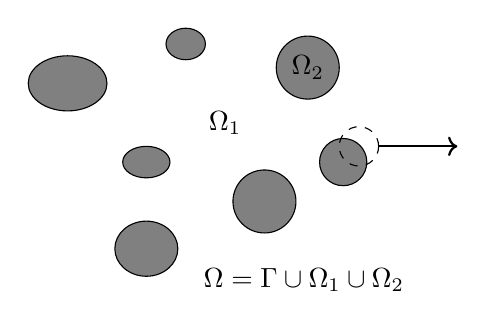
\begin{tikzpicture}
        \foreach \x/\y/\ra/\r in {
        1/3/0.2/0.25,
        2.55/2.7/0.4/0.4,
        0.5/0.4/0.35/0.4,
        2/1/0.4/0.4,
        3/1.5/0.3/0.3,
        0.5/1.5/0.2/0.3,
        -0.5/2.5/0.35/0.5}{
            \draw[fill=gray](\x,\y) ellipse(\r cm and \ra cm);
        }
        \draw[dashed](3.2,1.7)circle(0.25);
        % \draw[thick,->](3.2,1.7)++(0.1767,0.1767)--++(0.4,0.4)--++(1,0);
        \draw[thick,->](3.2,1.7)++(0.25,0)--++(1,0);
        \draw(2.55,2.7)node{$\Omega_2$};
        \draw(1.5,2)node{$\Omega_1$};
        \draw(2.5,0)node{$\Omega = \Gamma \cup \Omega_1 \cup \Omega_2$};
        % \draw(2.5,-1)node{$\Gamma = \sum_\alpha \Gamma_\alpha$};
        % \draw(2.5,-0.5)node{$\Omega_2 = \sum_\alpha \Omega_\alpha$};
    \end{tikzpicture}
    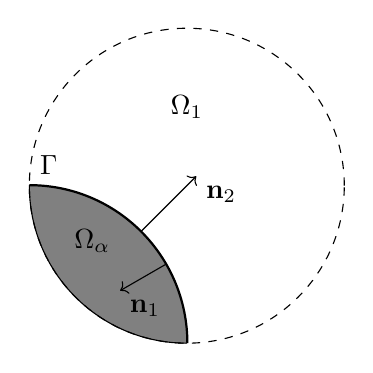
\begin{tikzpicture}%[scale = 0.9]
        \draw[very thick](0:2)arc(0:90:2)node[above right]{$\Gamma$};
        \draw[fill=gray](0:2)arc(0:90:2)arc(180:270:2);
        \draw[dashed](2,2)circle(2);
        \draw[->](1.42,1.42)--++(0.7,0.7)node[below right]{$\textbf{n}_2$};
        \draw[->](1.73,1)--++(-0.577,-0.333)node[below right]{$\textbf{n}_1$};
        \draw(2,3)node{$\Omega_1$};
        \draw(0.8,1.3)node{$\Omega_\alpha$};
    \end{tikzpicture}
    \caption{Topology of dispersed two-phase flows.}%Domain definitions and scheme of the topology of dispersed two-phase flows.}
    \label{fig:Scheme}
\end{figure}

We consider a system consisting of two phases, separated by a sharp interface $\Gamma(t)$ which evolves over time. 
For further insights into the modeling of sharp interface thermodynamics, a comprehensive review may be found in \cite{bothe2022sharp}. 
Each phase subdomain is denoted as $\Omega_1(t)$ and $\Omega_2(t)$, representing the continuous phase (1) and the dispersed phase (2) respectively (refer to Figure \ref{fig:Scheme}).
The entire domain, denoted as $\Omega$, is defined as the union of $\Omega_1$, $\Omega_2$, and $\Gamma$.
To track the position of the phase indexed $k$ and the interfaces, we introduce the phase indicator function $\chi _k$ defined as
\begin{align}
    \chi_k(\textbf{x},t) =  \left\{
      \begin{tabular}{cc}
        $1 \;\text{if} \;\textbf{x} \in \Omega_k(t)$\\
        $0 \;\text{if} \;\textbf{x} \notin \Omega_k(t)$
      \end{tabular}
      \right.
      \text{for $k = 1,2$}.
      \label{eq:PIF}
\end{align}


\subsection{Topological equations}
Using the distribution formalism, one may show that $\chi_k$ obeys the following relations \citep{drew1983mathematical,orlando2023evolution}. 
\begin{align}
    \pddt \chi_k
    + \textbf{u}_I^0 \cdot \grad \chi_k
    &= 0,
    \label{eq:dt_chi_k}\\
    \label{eq:grad_chi_k}
    \grad \chi_k
    &= - \delta_I \textbf{n}_k. 
\end{align}
where $u^0_I$ is the velocity of the interface and $\delta_I$ is the Dirac function localized on the interface.
Then, to describe the evolution of $\delta_I$ we take the gradient for \ref{eq:dt_chi_k} and the gradient of \ref{eq:grad_chi_k} which yields two equations of the interface indicator function \citep{marle1982macroscopic,morel2007surface,orlando2023evolution},
\begin{align}
    \pddt \delta_I
    + \div (\delta_I (\textbf{u}_I^0\cdot \textbf{n}) \textbf{n})
    &= \delta_I (\textbf{u}_I^0 \cdot \textbf{n})(\div\textbf{n})
    \label{eq:dt_delta_I}\\
    \grad\delta_I 
    &= \textbf{n} \cdot \grad (\textbf{n} \delta_I),
    \label{eq:grad_delta_I}
\end{align}
Notice that only the normal components of the surface velocity plays a role in this equation. 
We also employ the subscript $_I$ to indicate any quantity inherently defined on the interface such as its local velocity $\textbf{u}_I^0$. 

\ref{eq:dt_chi_k}, \ref{eq:dt_delta_I}, \ref{eq:grad_delta_I} and \ref{eq:grad_chi_k} are commonly referred to as the topological equations. 
It describes the evolution in space and time of the topology of the flow interfaces.
To enhance clarity, we will omit the time and position parameters from $\chi_k(\textbf{x},t)$ and $\delta_I(\textbf{x},t)$ in the subsequent sections.

\subsection{Local conservation equations}
\label{sec:local_eq}
Let now introduce the local conservation laws that govern the fluid inside bulk phases and the interfaces. 

\subsubsection{Inside the volumes}

Within phase $k$, we note $\rho_k$ the density, $\textbf{u}_k^0$ the local velocity and $E_k^0$ the local total energy per units of mass.
All over the domain $\Omega_k(t)$ the mass, momentum and total energy obey these conservation laws :
\begin{align}
    \label{eq:dt_rho}
    \pddt \rho_k  
    + \div (
        \rho_k\textbf{u}_k^0
    )
    &= 
    0\\
    \label{eq:dt_rhou_k}
    \pddt (\rho_k\textbf{u}_k^0)  
    + \div (
        \rho_k\textbf{u}_k^0\textbf{u}_k^0
        - \bm{\sigma}_k^0 
    )
    &= 
    \rho_k \textbf{g}\\
    \label{eq:dt_rhoE_k}
    \pddt (\rho_kE_k^0)  
    + \div (
        \rho_kE_k^0\textbf{u}_k^0
        + \textbf{q}_k^0
        - \textbf{u}_k^0 \cdot \bm{\sigma}_k^0 
        )
    &= 
    \textbf{u}_k^0 \cdot \textbf{g}  \rho_k
\end{align} 
All along this work the continuous phase will be considered as Newtonian fluid thus, $\bm{\sigma}_1^0 = - p_1^0 \bm\delta + \bm{\tau}_1^0$ where $\bm{\tau}_1^0$ is the Newtonian stress tensor with $p_1 ^0$ the local pressure and $\bm{\tau}_1^0 = \mu_1[\grad \textbf{u}_1^0+(\grad \textbf{u}_1^0)^T]$ the shear rate. 
The vector $\textbf{q}_k^0$ represent the thermal energy flux and is often model with a Fourier law : $\textbf{q}_k^0 = -\lambda \grad T_k^0$ where $T_k$ is the temperature and $\textbf{g}$ is the acceleration of gravity which will be the only body force in the present problem. 
All along this work the superscript $^0$ indicate that the variable is defied at the local or microscopic scale, in opposition to the averaged or macroscopic quantities that will be presented latter. 

The total energy is decomposed in the usual way, i.e. $E_k^0 = e_k^0 + (u_k^0)^2/2$ where  $e_k^0$ is the internal energy which represent the molecular agitation and $(u_k^0)^2/2$ is the kinetic energy per unit of mass.
This decomposition and the previous set of equations lead us to two independent equations for $e_k$ and $u_k$, namely,
\begin{align}
    \label{eq:dt_rhou_k2}
    \pddt [\rho_k(u_k^0)^2]  
    + \div [\rho_k(u_k^0)^2\textbf{u}_k^0/2 - \textbf{u}_k^0 \cdot \bm{\sigma}_k^0]
    &=
    \rho_k\textbf{u}_2^0 \cdot \textbf{g}  
    -  \bm{\sigma}_k^0 : \grad \textbf{u}_k^0,
    \\
    \label{eq:dt_rhoe_k}
    \pddt (\rho_ke_k^0)  
    + \div (
        \rho_ke_k^0\textbf{u}_k^0
        + \textbf{q}_k^0
        )
    &= 
    \bm{\sigma}_k^0 : \grad \textbf{u}_k^0. 
\end{align} 
We can observe that the viscous dissipation term, $\bm{\sigma}_k^0 : \grad \textbf{u}_k^0$,  appears with opposite sign in both of the above equations.
This indicates that $\bm{\sigma}_k^0 : \grad \textbf{u}_k^0$ is the energy that is transformed from kinetic to internal energy. 
By the use of thermodynamics equilibrium laws one can show that from the internal energy equation one can derive an equation for the local temperature \citet{ishii2010thermo}.
In this work we display the internal energy equation for completeness, no link with the temperature or any other thermodynamic quantity will be given. 
We will rather focus on the fluid and particle kinetic energy. 

\subsubsection{On interfaces}

\tb{
    dans cette section il y a une petite incoherence sur les equation energetique de surface. 
    En fait $E_I^0 = e_I^0 + (u_I^0)^2$ avec $e_I$ energie iinerne de surface qui est liée a la tension de surface par $\gamma = e_I − T_I s_I$ avec $T$ la temperature et $s$ l'entropie. bref faut que je mette tout ca au claire. 
    Pour résoudre le pbl voir\cite{ishii2010thermo}
}

On the interface $\Gamma(t)$ the conservation laws take the form of $2d$ conservation laws due to the topology of the interface. 
They are often viewed as \textit{jump condition} which make the link between the conservation equations in both phases. 
The interface mass and momentum conservation equation are well established.
However, the energy conservation law jump condition at the interface is less employed.
In the most general case the mass, momentum and energy surface equations can be written as\citep{morel2015mathematical}, 
\begin{align}
    \label{eq:dt_rhoI}
    \pddt \rho_I
    + \rho_I (\textbf{u}_I^0 \cdot \textbf{n})(\div \textbf{n})
    + \divI (\rho_I\textbf{u}_{I||}^0)
    &= 
    0
    % \Jump{
    %     \rho_k (\textbf{u}_I - \textbf{u}_k)
        % \mathbf{T}_k
    % }
    \\
    \label{eq:dt_rhoIu_I}
    \pddt (\rho_I\textbf{u}_I^0)  
    + \rho_I \textbf{u}_I^0 (\textbf{u}_I^0 \cdot \textbf{n})(\div \textbf{n})
    + \divI (
    \rho_I\textbf{u}_I^0\textbf{u}_{I||}^0
    - \bm{\sigma}_{I||}^0)
    &= 
    \rho_I \textbf{g}
    - \Jump{
        % \rho_k \textbf{u}_k (\textbf{u}_I - \textbf{u}_k)
        \bm\sigma^0_k
    }\\
    \label{eq:dt_rhoIE_I}
    \pddt (\rho_IE_I^0)  
    + \rho_IE_I^0  (\textbf{u}_I \cdot \textbf{n})(\div \textbf{n})
    + \divI (
        \rho_I E_I^0\textbf{u}_{I||}^0
        - \textbf{u}_I^0 \cdot \bm{\sigma}_I^0 
        + \textbf{q}_{I||}^0
        )
    &= 
    \textbf{u}_k^0 \cdot \textbf{g}  \rho_I
    - \Jump{\textbf{u}_k^0 \cdot \bm{\sigma}_k^0 - \textbf{q}_k^0}
\end{align} 
where, $\rho_I$ is the mass per unit of surface of the interface, $\textbf{u}_I^0$ is the local velocity of the interface $\Gamma(t)$, $\bm{\sigma}_I^0$ is the local momentum diffusive flux of surface, $\textbf{q}_I^0$ is the local internal energy diffusive flux of surface and $E_I^0 = e_I^0 + \frac{1}{2}(u_I^0)^2$ is the total energy at the interface, with $e_I^0$ the interface internal energy. 
We introduced the surface divergence operator defined as $\divI ()= (\bm\delta-\textbf{nn})\cdot \div ()$, which correspond to the divergence operator projected on $\Gamma(t)$. 
Throughout this work we use the subscript  $_{||}$ to indicate the projection of a quantity onto the plane tangential to the surface $\Gamma(t)$. 
Specifically, for an arbitrary quantity $\textbf{f}$ defined on $\Gamma(t)$, we denote its tangential projection as $\textbf{f}_{||}^0 = (\bm\delta-\textbf{nn})\cdot \textbf{f}^0$. 
Notice that the diffusive flux $\bm{\sigma}_{I||}^0$ and $\textbf{q}_{I||}^0$ appear as quantity projected on the surface tangential plane.
Indeed, it can be shown that only the tangential parts of the diffusive flux plays a role in the surface momentum balance equations, see \citet{slattery2007interfacial}.
We also introduced the notation $\Jump{\ldots}$, which is defined as $\Jump{\ldots} = \sum_{k=1}^2 [\ldots] \cdot \textbf{n}_k$.
Where $\textbf{n}_k$ is the outward normal vector associated with the domain $\Omega_k$ (see \ref{fig:Scheme}).

The formulations given by \ref{eq:dt_rho_I},\ref{eq:dt_rhoIu_I}and \ref{eq:dt_rhoI} remains quite general and needs some further simplifications. 
First we assume a thermodynamic local equilibrium everywhere at the interfaces. 
In this case the interfacial energy is closely related to the surface tension coefficient noted $\gamma$, that will be considered constant throughout this work. 
We assume that the momentum diffusive flux of surface is solely due to surface tension, therefore $\bm{\sigma}_I^0  = \gamma (\bm\delta - \textbf{nn}) = \gamma \bm\delta_{||}$ where $\gamma$ is the surface tension coefficient which will be assumed constant overall the interfaces \citep[Chapter 2]{tryggvason2011direct}.  
Note that in a more general case, interfacial viscous stress could be included into $\bm{\sigma}_{I}^0$ \citep{brenner2013interfacial,slattery2007interfacial,nadim1996concise}, nevertheless it will not be addressed in this study. 
Additionally, we assume the surface density to be negligible thus $\rho_I = 0$ and since we considered no energy accumulation at the interface $\textbf{q}_I=0$.
Also, instead of 
Consequently, the interfacial mass, momentum and total energy balance equations reduce to the common expressions :
\begin{align}
    \label{eq:dt_rho_I}
    \Jump{
        \rho_k (\textbf{u}_I - \textbf{u}_k)
        % \mathbf{T}_k
    }
    &=0, \\
    \Jump{\bm{\sigma}_k^0} 
    &=
    \divI\bm\sigma^0_{I||}
    =
    -\gamma\textbf{n}(\div \textbf{n}),
    % + \gradI\sigma 
    \label{eq:surface_tension}\\
    \label{eq:dt_rhoI_EI}
    - \Jump{\textbf{u}_k^0 \cdot \bm{\sigma}_k^0 - \textbf{q}_k^0}
    &=
    \pddt \gamma + \divI(\gamma \textbf{u}_I - \bm\sigma^0_{I||}\cdot \textbf{u}_I^0 )
    =
    + \gamma\textbf{n}\cdot \textbf{u}_{I}^0(\div \textbf{n}),
    % +
    % \label{eq:dt_rhoIe_I}
    % \Jump{ \textbf{q}_k^0}eq:dt_rho_I
    % &= 
    %  0
\end{align}
respectively. 
Where $ - \div\textbf{n}$ is twice the mean interface curvature.
% In \ref{eq:surface_tension}, we can clearly identify two contributions : the first one related to the curvature, and the second one from the non-constant surface tension coefficient along the surface. 
% The latter contribution is responsible for the Marangonie effect.
% This terms 
\ref{eq:dt_rhoI_EI} is the jump equation for the total energy.
However, in the following it will be more practical to deal with an equation for the kinetic and internal energy separately. 
Thus, we take the dot product of \ref{eq:surface_derivative}, \ref{eq:} with $\textbf{u}_I$ and subtract this new expression to \ref{eq:dt_rhoI_EI} which gives us, 
\begin{align}
    \label{eq:dt_rhoI_uI2}
    \Jump{\textbf{u}_k^0 \cdot \bm{\sigma}_k^0}
    &=
    -\gamma\textbf{n}\cdot \textbf{u}_{I}^0(\div \textbf{n})\\
    \label{eq:dt_rhoIe_I}
    \Jump{ \textbf{q}_k^0}
    &= 
     0
\end{align}
for the interface kinetic energy and the internal interface energy, respectively. 
Notice that this decomposition is possible only under the assumption of no mass transfer in which case $\textbf{u}_I^0=\textbf{u}_k^0$ for $k =1,2$ and a constant surface tension coefficient.


In the perspective of ensemble averaging the objective of the next two subsections is to extend the domain of definition of these two equations to the whole space $\Omega$.


\subsubsection{Generic formulation}

For ease of understanding, we now introduce generic conservation laws in the volumes and on the interfaces. 
Let $f_k^0(\textbf{x},t)$ denote a volumetric quantity of arbitrary tensorial order defined in $\Omega_k(t)$.
Likewise, let $f_I^0(\textbf{x}_I,I)$ represent an arbitrary surface property defined on $\Gamma(t)$.
Using the strategy outlined in \citep{bothe2022sharp,morel2015mathematical,slattery2007interfacial}, we can derive the local conservation equations for both $f_k^0(\textbf{x},t)$ and $f_I^0(\textbf{x}_I,t)$, that is,  
\begin{align}
    \label{eq:dt_f_k}
    \pddt f_k^0
    +\div \left(
        f_k^0\textbf{u}_k^0
        - \mathbf{\Phi}_k^0
        \right)
    &= 
    s_k^0
    & \text{ in } \Omega_k(t),&\\
    \pddt f_I^0 
    + f_I^0 (\textbf{u}_I \cdot \textbf{n})(\div \textbf{n})
    +\divI
    (f_I^0 \textbf{u}_{I||}^0
        - \mathbf{\Phi}_{I||}^0 )
    &= 
    s_I^0
    - \Jump{
       f_k (\textbf{u}_I^0 - \textbf{u}_k^0)
       + \mathbf{\Phi}_k^0
    } 
    & \text{ on } \Gamma(t),&
    \label{eq:dt_f_I}
\end{align}
respectively.
The tensors $\mathbf{\Phi}_k^0(f_k)$ and $\mathbf{\Phi}_{I||}^0(f_I)$ represent the non-convective fluxes corresponding to $f_k^0$ and $f_I^0$. 
Notice that $\mathbf{\Phi}_{I||}^0$ also carries the $_{||}$ subscript which implies that only the tangential component of this tensor remain in the surface balance equation. 
Similarly, $s_k^0(f_k^0)$ and $s_I^0(f_I^0)$ represent the source terms of $f_k^0$ and $f_I^0$, respectively.
Notice, that in \ref{eq:dt_f_I} we kept the mass transfer term $f_k (\textbf{u}_I^0 - \textbf{u}_k^0)$ for purpose of generality. 
For practical uses, note that the advecting term in \ref{eq:dt_f_I}can be written in the more compact form $f_I^0 (\textbf{u}_I \cdot \textbf{n})(\div \textbf{n})
+\divI(f_I^0 \textbf{u}_{I||}^0) = \divI(f_I^0 \textbf{u}_I^0)$ by noticing that $\textbf{n}\cdot\gradI(\ldots) = 0$ and $\divI\textbf{n} = \div\textbf{n}$ \citep{nadim1996concise}.
It is important to note that \ref{eq:dt_f_k} and \ref{eq:dt_f_I} are solely defined within $\Omega_k(t)$ and $\Gamma(t)$, respectively.
This was also the case for the equations presented in the last two subsections. 
Consequently, these equations are referred to as local conservation equations. 


\subsection{The two-fluid formulation}
The presence function $\chi_k$, and the Dirac delta function $\delta_I$, allow the extension of local conservation equations to the entire flow domain $\Omega$. 
This extension is achieved by employing the methodology introduced by \citet{drew1983mathematical} and \citet{kataoka1986local} for the conseriving laws inside the volume (\ref{eq:dt_f_k}).
For any local quantities $f_k^0$ defined in $\Omega_k(t)$, we assign the field $\chi_k f_k^0$, which is defined over the entire domain $\Omega$. The two-fluid formulation may be obtained by multiplying \ref{eq:dt_f_k} by $\chi_k$. 
Using \ref{eq:dt_chi_k} and \ref{eq:grad_chi_k} we obtain
\begin{equation}
    \pddt (\chi_k f_k^0)
    + \div (
        \chi_k f_k^0 \textbf{u}_k^0
        - \chi_k \mathbf{\Phi}_k^0 
        )
    = 
    \chi_k s_k^0
    + \delta_I\left[
        f_k^0
        \left(
            \textbf{u}_I^0
            - \textbf{u}_k^0
        \right)
        + \mathbf{\Phi}_k^0
    \right]
    \cdot \textbf{n}_k.
    \label{eq:dt_chi_k_f_k}
\end{equation}
Likewise, for any surface property $f_I^0$ defined on $\Gamma(t)$, we assign the field $\delta_I f_I^0$, which is also defined all over $\Omega$. 
Following the approach outlined \citet[Appendix 2]{marle1982macroscopic} we can generalize \ref{eq:dt_f_I} to the 3D space. 
Making use of the topological equations \ref{eq:dt_delta_I} and \ref{eq:grad_delta_I} gives,
\begin{equation}
    \pddt (\delta_If_I^0)  
    + \div (
        \delta_I f_I^0 \textbf{u}_I^0
        - \delta_I \mathbf{\Phi}_{I||}^0 
        )
    = 
    \delta_Is_I^0
    - \delta_I\Jump{
    f_k^0 (\textbf{u}_I^0 - \textbf{u}_k^0)
    + \mathbf{\Phi}_k^0} 
    \label{eq:dt_delta_I_f_I}
\end{equation}
which correspond to the conservation equation for $\delta_If_I^0$.
The last term on the right hands side of \ref{eq:dt_chi_k_f_k} represent the phase transfer of $f_k$ across the interfaces and the non-convective fluxes across phases.
The set of equations formed by \ref{eq:dt_chi_k_f_k} for $k =1,2$ is commonly known as the \textit{two-fluid} formulation of multiphase flows, to which we add the \textit{jump condition} across the phase given by \ref{eq:dt_delta_I_f_I} \citep{morel2015mathematical,tryggvason2011direct,drew1983mathematical,kataoka1986local}. 

\tb{this formulation is useful for the bulk stress}
In this work, we prefer to think of those equations as a set of three equations formed by \ref{eq:dt_chi_k_f_k} for $k=1,2$ and \ref{eq:dt_delta_I_f_I}. 
We define the \textit{bulk} property $\textbf{f}$ as $\textbf{f}^0 = \sum_k \chi_k \textbf{f}_k^0 + \delta_I \textbf{f}_I^0$ where $\textbf{f}^0$ represents any property of the flow of arbitrary tensorial order at the local scale.
Then by summing \ref{eq:dt_chi_k_f_k} for $k=1,2$ and \ref{eq:dt_delta_I_f_I}, one obtain the \textit{single-fluid} formulation conservation equation, namely,
\begin{equation}
   \pddt f^0
   + \div (
       f^0 \textbf{u}^0
       -  \mathbf{\Phi}^0 
    )
   = s^0. 
   \label{eq:dt_f}
\end{equation}
It should be noted that in the literature we rather define the \textit{bulk} quantities as $f^0 = \sum_k \chi_k f_k^0$, while the interfacial component is treated as a source term in \ref{eq:dt_f} \citep{morel2015mathematical,tryggvason2011direct,drew1983mathematical}. 
Nevertheless, we want to point out here that with this definition we recover a classic transport equation for the bulk quantity $f^0$ which makes the whole system of equation consistent.





Finally, we now expose the hybrid model for fluid particles. 
As stated before we do not consider mass transfer nor energy accumulation at the interface. 

\subsection{The averaged model}

Using the generic formulation \ref{eq:hybrid_avg_dt_chif} and the local expression of the mass, momentum and total energy expression, i.e. : \ref{eq:dt_rho},\ref{eq:dt_rhou_k} and \ref{eq:dt_rhoE_k} we easily find the averaged form of these equations as, 

\begin{align}
    \label{eq:dt_&vg_rho}
    \pddt (\phi_k \rho_k)  
    + \div (
        \phi_k \rho_k\textbf{u}_k
    )
    &= 
    0\\
    \label{eq:dt_&vg_rhou_k}
    \pddt (\phi_k \rho_k\textbf{u}_k)  
    + \div (
        \phi_k \rho_k\textbf{u}_k\textbf{u}_k
        - \bm{\sigma}_k^\text{eq}
    )
    &= 
    \phi_k \rho_k \textbf{g} 
    +  \avg{\delta_I \bm{\sigma}_k^0 \cdot \textbf{n}_k}\\
    \label{eq:dt_&vg_rhoE_k}
    \pddt (\phi_k\rho_kE_k)  
    + \div (
        \phi_k\rho_kE_k\textbf{u}_k
        + \bm{q}_k^\text{eq}
        - \textbf{u}_k \cdot \bm{\sigma}_k^\text{eq}
        % - \textbf{u}_k^0 \cdot \bm{\sigma}_k^0 
        % + \textbf{q}_k^0
        )
    &= 
    \phi_k \rho_k\textbf{u}_k \cdot \textbf{g} 
    + \avg{\delta_I (\textbf{u}_k^0 \cdot \bm{\sigma}_k^0 - \textbf{q}_k^0)\cdot \textbf{n}_k}
\end{align} 
\todo{Is this formulation usefull for the NRJ equaiton ? }
where we have defined, 
\begin{align*}
    &\bm{\sigma}_k^\text{eq}
    = \phi_k\rho_k (
        \bm{\sigma}_k%- n_p \textbf{M}_p
        - \kavg{\textbf{u}_k'\textbf{u}_k'})  
    &\textbf{q}_k^\text{eq}
    = \phi_k\rho_k \kavg{\textbf{u}_k' e_k' + \textbf{u}_k' k_k} - \phi_k\kavg{\textbf{u}_k' \cdot \bm{\sigma}_k^0}
    + \phi_k\textbf{q}_k \\
\end{align*}
Note that the phase averaged energy equation can be further decompose following, 
\begin{align*}
    E_1 = e_1 + k_1 + u_k^2/2\\
    % E_1'= e^0_1 + (u_1^0)^2 - (e_1 + k_1 + u_k^2/2) = 
    % e_1' + (u_1^0)^2/2 - (k_1 + u_k^2/2)\\
    % \oneavg{E_1'\textbf{u}_1'}
    % = 
    % \oneavg{\textbf{u}_1' e_1'}
    % + \oneavg{u_1'[(u_1^0)^2/2 - u_k^2/2] }
    % - \oneavg{u_1' k_1} \\
    % \oneavg{E_1'\textbf{u}_1'}
    % = 
    % \oneavg{\textbf{u}_1' e_1'}
    % + \oneavg{\textbf{u}_1' \textbf{u}_1'} \cdot \textbf{u}_1 
    % + \oneavg{u_1'(u_1^0)^2/2 }
    % - \oneavg{u_1' k_1} \\
    \oneavg{E_1^0\textbf{u}_1'}
    = 
    E_1\oneavg{\textbf{u}_1'}
    + \oneavg{E_1'\textbf{u}_1'}
    = 
    \oneavg{\textbf{u}_1' e_1^0}
    + \textbf{u}_1 \cdot \oneavg{\textbf{u}_1'  \textbf{u}_1'}
    +\oneavg{\textbf{u}_1' k_1 }\\
    - \avg{\chi_k(\textbf{u}_k^0 \cdot \bm{\sigma}_k^0 - \textbf{q}_k^0)}
    =- \phi_k (\textbf{u}_k \cdot \bm{\sigma}_k - \textbf{q}_k) 
    - \phi_k \kavg{\textbf{u}_k' \cdot \bm{\sigma}_k^0}
\end{align*}
where $K_1$ is the pseudo-turbulent kinetic energy defined such as, $\phi_1 k_1 = \avg{\chi_1 (u_1')^2/2}$. 
The Macroscopic kinetic energy equation can be obtain by taking the dot product with $\textbf{u}_k$. 
\begin{align}
    \pddt (\phi_k \rho_ku_k^2/2)  
    + \div (
        \phi_k \rho_k\textbf{u}_ku_k^2/2
        - \textbf{u}_k \cdot \bm{\sigma}_k^\text{eq}
    )
    &= 
    - \bm{\sigma}_k^\text{eq} : \grad \textbf{u}_k
    + \phi_k \rho_k \textbf{u}_k\cdot \textbf{g} 
    +  \textbf{u}_k\cdot \avg{\delta_I \bm{\sigma}_k^0 \cdot \textbf{n}_k}\\
    \pddt (\phi_k\rho_kk_k)  
    + \div (
        \phi_k\rho_kk_k\textbf{u}_k
        + \phi_k\rho_k \kavg{\textbf{u}_k' k_k} 
        - \phi_k\kavg{\textbf{u}_k' \cdot \bm{\sigma}_k^0}
        )
    &= 
    - \avg{\chi_k\bm{\sigma}_k^0 : \grad \textbf{u}_k^0}
    + \bm{\sigma}_k^\text{eq} : \grad \textbf{u}_k
    + \avg{\delta_I \textbf{u}_k' \cdot \bm{\sigma}_k^0 \cdot \textbf{n}_k}\\
    \pddt (\phi_k\rho_ke_k)  
    + \div (
        \phi_k \rho_ke_k\textbf{u}_k
        +
        \phi_k \rho_k\oneavg{e_k'\textbf{u}_k'}
        + \phi_k\rho_k\textbf{q}_k
        )
    &= 
    \avg{\chi_k\bm{\sigma}_k^0 : \grad \textbf{u}_k^0}
    - \avg{\delta_I \textbf{q}_k^0 \cdot \textbf{n}_k} 
\end{align}



mu_r**(-1)

\section{Lagrangian equations of conservation to model the dispersed phase}
\label{sec:Lagrangian}

While \ref{eq:dt_chi_k_f_k} and \ref{eq:dt_delta_I_f_I} describe multiphase-flow in a general manner, they do not leverage the topology of the dispersed phase. 
Therefore, in this section, we present a Lagrangian-based model capable of describing the dispersed phase with an arbitrary order of accuracy.

\subsection{Fundamental properties}

At this stage, it is crucial to define some fundamental properties associated to each particle.
Following the strategy of \citet{lhuillier2009rheology,lhuillier1992volume,zaepffel2011modelisation} and \citet[Chapter 2]{morel2015mathematical}
we define the mass, position of center of mass, momentum and total energy of the particle $\alpha$, such as,
\begin{align}
    &m_\alpha(t)
    = \int_{\Omega_\alpha(t)} \rho_2  d\Omega,
    % &&
    &\textbf{x}_\alpha(t)
    = \frac{1}{m_\alpha(t) }\int_{\Omega_\alpha(t)} \rho_2 \textbf{x} d\Omega,\\
    % &&
    &\textbf{p}_\alpha(t) 
    = \int_{\Omega_\alpha(t)} \rho_2 \textbf{u}_2^0 d\Omega,
    % &&
    & m_\alpha E_\alpha(t) 
    = \int_{\Omega_\alpha(t)} \rho_2 [e_2^0 + (u_2^0)^2/2] d\Omega,
    \label{eq:position_and_momentum_def}
\end{align}
respectively. 
Where $\Omega_\alpha$ is the domain occupied by the particle $\alpha$ (see \ref{fig:Scheme}). 
Subsequently, we define the velocity of the particle's center of mass, denoted as $\textbf{u}_\alpha$ which is given by $\textbf{u}_\alpha = \ddt \textbf{x}_\alpha$. 
The derivation of $\ddt \textbf{x}_\alpha$ is straightforward but requires some algebra which are detailed in \ref{ap:velocity_definition}. 
The final expression reads,
\begin{equation}
    \textbf{u}_\alpha(t) = \frac{1}{m_\alpha(t)} \left(
        \textbf{p}_\alpha(t)
        +  \int_{\Sigma_\alpha(t)} \rho_2 \textbf{r} (\textbf{u}_I^0 - \textbf{u}_2^0)\cdot \textbf{n}_2 d\Sigma
        \right),
        \label{eq:dt_y_alpha}
\end{equation}
where $\textbf{r}(\textbf{x},t) = \textbf{x} - \textbf{x}_\alpha(t)$. 
In Equation \ref{eq:dt_y_alpha}, it can be observed that the first component of the velocity represents the linear momentum divided by the mass of the particle. 
This corresponds to the mass-averaged velocity over the volume of the particle.
The second term in Equation \ref{eq:dt_y_alpha} arises from the contribution of anisotropic mass transfer across the surface of the particle. 
This mass transfer leads to the motion of the particle's center of mass, thereby contributing to the total velocity.
To illustrate this concept, let us consider a fixed drop with no momentum lying over a very hot plate.
In this scenario, we assume that the plate is sufficiently hot to induce evaporation, specifically on the bottom portion of the drop.
Hence, under the effect of an anisotropic evaporation flux one may expect the second term to be non-negligible.
Consequently, the center of mass of the drop has a non-zero velocity in the opposite direction of the plate, even though the momentum is assumed to be zero.
We can also consider the case of the nucleation of a bubble in water. 
In this case, although the particle momentum is null at all time the center of mass of the particle moves due to the growth of the particle. 
In both cases, we need to take into account the mass transfer term in \ref{eq:dt_y_alpha}, while the first term is negligible. 
Note that \ref{eq:dt_y_alpha} generalized usual expression of the center of mass velocity whom neglect the second term.
In the following, we discard the time dependency notation for all Lagrangian quantities denoted by the subscript $_\alpha$ and also $\Sigma(t)$ and $\Omega_\alpha$.
Nevertheless, the reader must understand that all Lagrangian quantities and integration domains subscribed by $_\alpha$ are time dependent. 

The particle's internal relative motions or the \textit{inner velocity} is given by $\textbf{w}_2^0(\textbf{x},t) = \textbf{u}_2^0(\textbf{x}) - \textbf{u}_\alpha(t)$.
Thus, from its definition in \ref{eq:position_and_momentum_def}, we can rewrite the momentum as follows,
\begin{equation}
    \label{eq:momentum_definition_1}
    \textbf{p}_\alpha
    = m_\alpha \textbf{u}_\alpha
    + \int_{\Omega_\alpha} \rho_2 \textbf{w}_2^0 d\Omega.
\end{equation}
Alternatively, by manipulating \ref{eq:dt_y_alpha}, we obtain,
\begin{equation}
    \textbf{p}_\alpha
    =  m_\alpha \textbf{u}_\alpha
    - \int_{\Sigma_\alpha} \rho_2\textbf{r}(\textbf{u}_I^0 - \textbf{u}_2^0)\cdot \textbf{n}_2 d\Sigma
    \label{eq:momentum_definition}
\end{equation}
Therefore, the momentum of a particle can be seen as a sum of the mean velocity plus the integral of the fluctuation (\ref{eq:momentum_definition_1}), with the latter being equivalent to minus the first moment of mass transfer term (\ref{eq:momentum_definition}).
Indeed, by identification we obtain : $\int_{\Omega_\alpha} \rho_2 \textbf{w}_2^0 d\Omega =\int_{\Sigma_\alpha}  \rho_2\textbf{r} (\textbf{u}_I^0 - \textbf{u}_2^0)\cdot \textbf{n}_2 d\Sigma$. 
The essential aspect of this relation highlighted here is that the internal velocity fluctuations within a fluid particle do not contribute to the total linear momentum $\textbf{p}_\alpha$, as long as the anisotropic mass transfer is negligible.  
Additionally, the total energy $E_\alpha$ can be decomposed following a similar procedure which leads us to, 
\begin{equation*}
    \label{eq:E_alpha_def}
    m_\alpha E_\alpha(t) 
    = m_\alpha e_\alpha 
    + W_\alpha
    + m_\alpha (u_\alpha)^2/2
    % + \textbf{u}_\alpha \cdot \int_{\Omega_\alpha(t)} \rho_2  \textbf{w}_2^0 d\Omega
\end{equation*}
where we introduced the internal kinetic energy : $W_\alpha = \int_{\Omega_\alpha(t)} \rho_2  (w_2^0)^2/2 d\Omega$. 
In that expression mass transfer have been neglected. 
Anyhow, the total energy of a particle is the sum of its internal energy $e_\alpha$, internal kinetic energy $W_\alpha$ and the kinetic energy  due to its own center of mass displacement $u_\alpha^2/2$. 
To gain in understanding, let's express $W_\alpha$ in the case of a solid particle.
The velocity inside a solid particle can be expressed : $\textbf{u}_2^0(\textbf{x}_\alpha + \textbf{r}) = \textbf{u}_\alpha + \textbf{r}\times \bm{\omega}_\alpha$ where $\bm{\omega}_\alpha$ is the angular velocity.  
In this case, $W_\alpha = \bm{\omega}_\alpha\bm{\omega}_\alpha\cdot \mathcal{I}_\alpha$ where $\mathcal{I}_\alpha$ is the inertia matrices of the particle. 
As a matter of facts for solid particles $W_\alpha$ represents the angular kinetic energy for solid particles.
Thus, for particles with fluid internal motion, $W_\alpha$ is just a more general definition of the particle internal kinetic energy. 

\subsection{Conservation laws}
We assign to a particle indexed, $\alpha$, occupying the domain $\Omega_\alpha$ (see \ref{fig:Scheme}) an arbitrary Lagrangian property $q_\alpha$ defined by $q_\alpha  = \int_{\Omega_\alpha} f_2^0(\textbf{x},t) d\Omega$.
Similarly, we define $q_{I\alpha} = \int_{\Sigma_\alpha} f_I^0(\textbf{x},t) d\Sigma$ as being an integrated surface property associated to the particle $\alpha$.


To describe the evolution of any arbitrary Lagrangian quantity $q_\alpha$, we need to establish its time derivative.
Since, $q_\alpha$ is an integral quantity with a time-dependent domain of integration, we apply the general Reynolds transport theorem for volume integral (exposed in \ref{ap:math}) to compute its time derivative \citep{morel2015mathematical}.
This yields the following expression :
\begin{equation}
    \ddt  q_\alpha
    = \int_{\Omega_\alpha}\left[ \pddt f_2^0 + \div\left(f_2^0\textbf{u}_2^0\right) \right]d\Omega\\
    + \int_{\Sigma_\alpha} f_2^0 (\textbf{u}_I^0-\textbf{u}_2^0)\cdot \textbf{n}_2 d\Sigma.
\end{equation}
By substituting the integrand of the first integral on the right-hand side (RHS) with \ref{eq:dt_f_k} we obtain the conservation laws of the quantity $q_\alpha$, namely,  
\begin{equation}
    \ddt  q_\alpha
    = \int_{\Omega_\alpha} s_2^0 d\Omega
    + \int_{\Sigma_\alpha} \left[
        f_2^0 (\textbf{u}_I^0-\textbf{u}_2^0) 
        + \mathbf{\Phi}_2^0 
        \right] \cdot \textbf{n}_2 d\Sigma,
    \label{eq:dt_q_alpha}
\end{equation}
The first term on the RHS accounts for the total contribution of the source term $s_2^0$ to the particle $\alpha$.
While, The second term on the RHS is the surface integration of the exchange terms, which includes the phase transfer flux $f_2^0 (\textbf{u}_I^0-\textbf{u}_2^0)$ and the diffusive flux $\mathbf{\Phi}_2^0$. 
For clarity, let us consider the specific case of the momentum balance, i.e. when $q_\alpha = \textbf{p}_\alpha$.
In this situation, the first term reads as $\int_{\Omega_\alpha} \rho_2\textbf{g} d\Omega$ and represents the total weight acting on the particle $\alpha$. 
Likewise, the second term represents the total source of momentum due to phase transfer, and it is expressed as, $\int_{\Sigma_\alpha} \rho_2 \textbf{u}_2^0 (\textbf{u}_I^0-\textbf{u}_2^0)\cdot\textbf{n}_2 d\Sigma$. 
Lastly, $\int_{\Sigma_\alpha} \bm{\sigma}_2^0\cdot\textbf{n}_2 d\Sigma$ represents the resultant of the hydrodynamic forces acting on the surface of the particle.
It is important to notice that under this form, the exchange terms are expressed as integrals of dispersed phase fields denoted by the subscript $_2$.
Nevertheless, depending on the nature of the dispersed phase, these fields may not always be defined.
For infinitely rigid particles it is indeed the case since, the stress $\bm{\sigma}_2^0$ isn't defined.  
Hence, our objective is to express these exchange terms, in terms of the continuous phase field quantities instead of the dispersed phase field, i.e. in terms of $\mathbf{\Phi}_1^0$ and $\textbf{u}_1^0$ rather than $\mathbf{\Phi}_2^0$ and $\textbf{u}_2^0$. 

To address this issue, let us derive the conservation equation for the integrated surface property $q_{I\alpha}$.
To differentiate time-varying surface integrals within time, we can use the general Leibniz rule (see \ref{eq:Leibnitz}), to derive the following expression :
\begin{equation}
    \ddt  q_{I\alpha}
    = \int_{\Sigma_\alpha} \left[
        \pddt f_I^0
        +   \gradI \cdot (\textbf{u}_I^0f_I^0)
    \right]d\Sigma.
    \label{eq:surface_derivative}
\end{equation}
Substituting the RHS terms of \ref{eq:surface_derivative} using \ref{eq:dt_f_I}, and making use of the surface divergence theorem on closed surfaces (see \ref{eq:surf_div_theorem}), gives,
\begin{equation}
    \ddt  q_{I\alpha}
    = \int_{\Sigma_\alpha} 
        s_I^0
    d\Sigma
    - \int_{\Sigma_\alpha} \Jump{
        f_k^0 (\textbf{u}_I^0 - \textbf{u}_k^0)
        + \mathbf{\Phi}_k^0
    }
    d\Sigma.
    \label{eq:dt_q_I_alpha}
\end{equation}
This equation can be interpreted as the surface conservation equation for the integrated surface property $f_I$, or as the flux jump condition integrated on a closed surface. 
Notice that $\bm{\Phi}_{I}^0$ isn't present in this balance equation. 
This is due to the fact that as mentioned earlier, only the tangential components of $\bm{\Phi}_{I}^0$ appear inside the surface balance equation, while we perform an integration over a closed surface which is null due to \ref{eq:surf_div_theorem}. 

As discussed above we wish to get rid of $\mathbf{\Phi}_2^0$ in \ref{eq:dt_q_alpha}. To achieve this, we treat the particle's volume and surface as a unified entity and derive a conservation equation for $q_\alpha^\text{tot} = q_\alpha + q_{I\alpha}$. 
This is done by summing \ref{eq:dt_q_alpha} and \ref{eq:dt_q_I_alpha} which leads to, 
\begin{equation}
    \ddt  q_\alpha^\text{tot}
    = 
    \int_{\Omega_\alpha} s_2^0 d\Omega
    + \int_{\Sigma_\alpha} s_I^0 d\Sigma
    + \int_{\Sigma_\alpha} \left[
        f_1^0 (\textbf{u}_I^0-\textbf{u}_1^0) 
        + \mathbf{\Phi}_1^0 
        \right] \cdot \textbf{n}_2 d\Sigma. 
    \label{eq:dt_q_alpha_tot}
\end{equation}
This equation is the general form of the linear conservation law of $\chi_2 f_2^0 + \delta_I f_I^0$ for the system consisting of the particle volume $\Omega_\alpha$, and its surface $\Sigma_\alpha$. It is applicable to any particle immersed into a continuous phase following the local conservation,\ref{eq:dt_f_k} and \ref{eq:dt_f_I}.
We refer to this equation as the zeroth-order conservation equation or the linear conservation law for the particle $\alpha$.

Following the same assumption as in \ref{sec:local_eq}, i.e. we consider no mass transfer and weightless interfaces, the Lagrangian  mass, momentum and energy equations for a single particle can be derived using the generic form \ref{eq:dt_q_alpha_tot} and reads as, 
\begin{align}
    \label{eq:dt_m_alpha}
    \ddt m_\alpha
    &= 
    0\\
    \label{eq:dt_p_alpha}
    \ddt (m_\alpha \textbf{u}_\alpha)
    &= 
    m_\alpha\textbf{g}
    +  \intS{\bm{\sigma}_2^0 \cdot \textbf{n}_2}\\
    \label{eq:dt_E_alpha}
    \ddt (m_\alpha E_\alpha + s_\alpha \gamma)
    &= 
    m_\alpha \textbf{u}_\alpha \cdot \textbf{g}
    +\textbf{u}_\alpha \cdot \intS{\bm{\sigma}_2^0 \cdot \textbf{n}_2}   
    +\intS{\textbf{w}_1^0 \cdot \bm{\sigma}_1^0 \cdot  \textbf{n}_2} 
    - \intS{\textbf{q}_2^0 \cdot \textbf{n}_2}
\end{align}
where  $\int_{\Sigma_\alpha}  \bm{\sigma}_1^0 \cdot \textbf{n}_2 d\Sigma$ is the resultants of the hydrodynamic force and $\int_{\Sigma_\alpha} \textbf{q}_1^0 \cdot \textbf{n}_2 d\Sigma$ is the resultants of the surface heat flux. 
The second term on the right hands side of the energy equation is the work produced by the mean force and the translational motion of the droplets, while $\intS{\textbf{w}_1^0 \cdot \bm{\sigma}_1^0 \cdot  \textbf{n}_2}$ is the work produced by the local forces and local motion of the fluid at the surface of the particle.
Since we integrated the energy over the particle's volume and its surface, we explicitly made appear the surface energy $\gamma s_\alpha$ within the derivative operator. 
Note that these equations does not explicitly account for inter-particle interactions. 
However, it is possible to include manually such forces by noticing that the surface external stress flux $\bm{\sigma}_1^0$ is the sum of hydrodynamic and particles-particles interaction forces, regardless it is pure contact forces from direct contact or a force mediated through the carrier fluid.
From this consideration it is possible to split every term involving the stress $\bm{\sigma}_1^0$ into two terms representing these contributions. 
Same comments can be made for the heat flux $\textbf{q}_1^0$. 
Although this distinction is important, for purpose of clearly we will stay general, and we will keep the fluxes $\bm{\sigma}_1^0$ and $\textbf{q}_1^0$ as such. 

In the spirit of the energy decomposition exposed in \ref{eq:E_alpha_def} the total energy equation can be split into three equations, one for the center of mass kinetic energy, internal motion and internal kinetic energy, namely,  
\begin{align}
    \label{eq:dt_u2_alpha}
    \frac{1}{2}\ddt (m_\alpha u_\alpha^2)
    &= 
    \textbf{u}_\alpha\cdot
    \textbf{g}m_\alpha
    + 
    \textbf{u}_\alpha\cdot
    \textbf{f}_\alpha,\\
    \label{eq:dt_w2_alpha}
    \ddt W_\alpha 
    &= 
    \intS {\textbf{w}_1^0 \cdot \bm{\sigma}_1^0 \cdot \textbf{n}_2 }
    - \intO{ \bm{\sigma}_2^0 : \grad\textbf{u}_2^0 }
    - \ddt (s_\alpha \gamma) 
    \\
     \label{eq:dt_e_alpha}
    \ddt (m_\alpha e_\alpha )
    &= 
     \intO{ \bm{\sigma}_2^0 : \grad\textbf{u}_2^0  }
    -  \intS{\textbf{q}_1^0\cdot \textbf{n}_2 } 
\end{align}
respectively. 
Note that in \citet{eq:dt_w2_alpha} the use of \ref{eq:dt_rhoI_uI2} makes appear explicitly the derivative of the surface energy $s_\alpha \gamma$. 
Note that under this form we see that the energy loss in the deformation represented by $W_p$ will be gathered in the surface energy which will in turn act as a source term in the internal kinetic energy motion.
The surface tension plays the role as a spring in the energy balance.   
From this set of equation we can easily see that the rate of dissipation terms $\intS{\bm{\sigma}_2^0 : \grad\textbf{u}_2^0}$ represent an energy sink in the equation of $W_\alpha$ while it is a source term in the internal energy equation. 
As it has been observed in the previous section, this terms convert the energy of internal motion to molecular agitation. 
However, the interplay between the center of mass  kinetic energy and the internal fluctuation is not obvious and has no common term with the heat and internal kinetic energy equation.
In fact, we will see that the transfer between these scales is archived thought the fluid phase pseudo turbulent energy. 


Finally, we would like to highlight that  due to the consideration of closed surface, the diffusive flux $\mathbf{\Phi}_I$, plays no role at all in \ref{eq:dt_q_alpha_tot}.
Therefore, in the case of the linear momentum conservation law, the contribution of the surface tension forces exposed in \ref{eq:surface_tension}, do not contribute to the momentum balance in \ref{eq:dt_p_alpha}.
As a consequence, even in the presence of local Marangoni forces, the resultant of the local surface tension forces cancels out in the linear momentum balance.
This fact has already been demonstrated by \citet{hesla1993note} who showed that the surface tension force does not contribute to the linear and angular momentum balance. 
Here, we have provided the general proof that the interfacial diffusive flux $\mathbf{\Phi}_I^0$, which is present at the local scale according to \ref{eq:dt_f_I}, does not contribute to the zeroth-order conservation law of a particle with a closed surface.
This is therefore applicable to other conservation equations, such as the surface energy balance or the surface mass balance of constituents, where surface diffusive fluxes are also present \citep{bothe2022sharp,manikantan2020surfactant}. 

Nevertheless, it is known that surface tension forces impact the hydrodynamic of droplets and bubbles \citep{kentheswaran2022direct,pesci2018computational}. 
Therefore, if the diffusive flux of surface are not involved in the linear conservation law, it must appear at some point in the momentum description of Lagrangian particles. 
To find out where this contribution arise we shall describe the particle with a higher level of accuracy. 
This is the purpose of the next section. 

\subsection{First order moment equations}

To better describe the local properties within the particles, we now introduce the first moment or the dipole of a particle.
We define the first moment of any properties $f_2^0$ and $f_I^0$ by respectively,
\begin{align}
    &\mathcal{Q}_\alpha 
    = \int_{\Omega_\alpha} \textbf{r} f_2^0 d\Omega,
    &\text{and}&
    &\mathcal{Q}_{I\alpha}
    = \int_{\Sigma_\alpha} \textbf{r} f_I^0 d\Sigma,
    \label{eq:first_moment_definition}
\end{align}
where we recall that $\textbf{r} = \textbf{x} - \textbf{x}_\alpha$ is the distance between any point inside $\Omega_\alpha$ or $\Sigma_\alpha$, to the center of mass of the particle $\alpha$.
It is then possible to differentiate these moments with respect to time in order to obtain their conservation laws.
Indeed, considering \ref{eq:dt_f_k}, \ref{eq:dt_f_I} and applying the Leibniz rule for volume and surface integrals (see \ref{eq:Reynolds} and \ref{eq:Leibnitz} respectively), we can show equally that,
\begin{align}
    \ddt \mathcal{Q}_\alpha
    &= \int_{\Omega_\alpha} \left(
        \textbf{r} s_2^0         
        + f_2^0  \textbf{w}_2^0 
        - \mathbf{\Phi}_2^0
    \right) d\Omega,
    + \int_{\Sigma_\alpha} \textbf{r} \left[
        \mathbf{\Phi}_2^0
        + f_2^0 (\textbf{u}_I^0-\textbf{u}_2^0)
    \right]\cdot \textbf{n}_2  d\Sigma 
    \label{eq:dt_Q_alpha}\\
    \ddt \mathcal{Q}_{I\alpha}
    &= \int_{\Sigma_\alpha} \left(
        \textbf{r}s_I^0
        + f_I^0 \textbf{w}_I^0
        - \mathbf{\Phi}_{I||}^0
    \right) d\Sigma,
    - \int_{\Sigma_\alpha}\textbf{r} 
    \Jump{\mathbf{\Phi}_k^0
        + f_k^0 (\textbf{u}_I^0 - \textbf{u}_k^0)
    }
    d\Sigma
    \label{eq:dt_Q_I_alpha}
\end{align}
where $\textbf{w}_I^0 = \textbf{u}_I^0 - \textbf{u}_\alpha$.
The detailed derivation of \ref{eq:dt_Q_alpha} is provided in \ref{ap:moment_derivative}.
The derivation of \ref{eq:dt_Q_I_alpha} follows a similar procedure. 
% \JL{je n'ai pas relu la derivation detaillee en annexe, ... je te fais confiance. par contre en annexe tu ne derive pas le premier moment interfacial. 
% J'imagine que la derivation est la meme encore faut il le preciser. 
% Egalement j'ai regorganise les elements dans les equations precedentes par signification physique. 
% D'ailleurs il y avait des differences dans les deux equations (la premiere $r S$, la seconde $S r$)... 
% Merci de faire attention a ce genre de detail. 
% J'avoue avoir du mal a comprendre l'interpretation physique de l'integrale de la contrainte dans le volume. 
% Comme on en discutait, par exemple pour une particule solide, celle integrale n'est pas determinee, donc il faudrait la remplacer par quelque chose que l'on connait non ? 
% \tb{Dans le cas ou les contrainte ne sont pas defini les degrées de liberté des particules solid font que cette contrainte ne peux ne pas etre prise en compte la partie symmetrique de cette formule 
% permet justement de remonter a la contrainte dans le cas ou elle ne serait pas defini. dans le cas des particue fluid cela a du sens parcontre c'est les contraintes interne qui s'oppose a la deformations}}
% \JL{
%  Enfin bon a discuter (pas forcement ici). 
%  je pense que c'est un point important. 
% }\tb{cela va etre discuter dans la partie ou on traitre du momentum non ?}
% \JL{
%  Par ailleurs dans quel cas l'integrale des fluctuations $w_2$ est elle nulle ? 
%  pour une particule solide est ce le cas ? 
%  j'imagine que oui ? 
%  J'imagine que tout cela est traite plus tard (dans la derniere section), mais ca me parait crucial de bien expliquer a quoi servent ces termes et dans quel cas ils sont nuls. 
%  \tb{dur a expliquer pour une quantité general }
%  }\JL{
%  Une maniere d'expliciter tout cela pourrait etre de separer j'imagine le premier moment (au moins pour la vitesse) en une partie symmetrique et une partie anti symmetrique pour bien differencier ce qui est lie a la vitesse angulaire et la deformation. 
%  \tb{dans ce cas il faudrait donner l'application du momentum maintenant ce qui change le plan}}
In \ref{eq:dt_Q_alpha}, we recognize the first moment of the source term $s_2^0$, the first moment of the diffusive flux term $\mathbf{\Phi}_2^0\cdot\textbf{n}_2$ and the first moment of phase exchange term, $f_2^0 (\textbf{u}_I^0-\textbf{u}_2^0)\cdot\textbf{n}_2$. 
Additionally, two supplementary terms appear in \ref{eq:dt_Q_alpha}, namely : the integral of the diffusive flux $\mathbf{\Phi}_2^0$, and a term related to the fluctuation of the internal velocity $f_2^0 \textbf{w}_2^0$.
Similar observations can be made for the fist moment of surface equation \ref{eq:dt_Q_I_alpha}, as it shares similarities with \ref{eq:dt_Q_alpha}. 
In particular, it is worth noting the presence of the surface diffusive flux $\mathbf{\Phi}_{I||}^0$ in \ref{eq:dt_Q_I_alpha}.
This term will be further discussed and analyzed in the following. 

For similar reason than the linear conservation equations, we sum \ref{eq:dt_Q_alpha} and \ref{eq:dt_Q_I_alpha} to expresses the conservation equation of the total first moment $\mathcal{Q}_\alpha^\text{tot} = \mathcal{Q}_\alpha + \mathcal{Q}_{I\alpha}$.
This leads to the following expression:
\begin{multline}
    \ddt \mathcal{Q}_\alpha^\text{tot}
    = \int_{\Omega_\alpha} \left(
        \textbf{r} s_2^0         
        + f_2^0  \textbf{w}_2^0 
        - \mathbf{\Phi}_2^0
    \right) d\Omega\\
    + \int_{\Sigma_\alpha} \left(
        \textbf{r}s_I^0
        + f_I^0 \textbf{w}_I^0
        - \mathbf{\Phi}_{I||}^0
    \right) d\Sigma
    + \int_{\Sigma_\alpha} \textbf{r} \left[
        \mathbf{\Phi}_1^0
        + f_1^0 (\textbf{u}_I^0-\textbf{u}_1^0)
    \right]\cdot \textbf{n}_2  d\Sigma.
    \label{eq:dt_Q_alpha_tot}
\end{multline}
Likewise, conservation laws can be derived for an arbitrary $n^{th}$ order moments of volume and surface, i.e. for
\begin{align}
    \mathcal{Q}_\alpha^n
    = \int_{\Omega_\alpha}
        \textbf{r}^n
        f_2^0 d\Omega,
        && \text{and} &&
    \mathcal{Q}_{I\alpha}^n
    = \int_{\Sigma_\alpha}
        \textbf{r}^n
    f_I^0 d\Sigma,
    \label{eq:Q_n_definition}
\end{align} 
respectively, where $\textbf{r}^n$ is the shorthand for the tensor product $\textbf{r}^n = \underbrace{\textbf{rr}\ldots \textbf{rr}}_{n\text{ times}} $ with $n$ times itself. 
It can be shown that the derivative with time of do not involve any additional terms than in \ref{eq:dt_Q_alpha} and \ref{eq:dt_Q_I_alpha}, but rather just the $n^{th}$ order moments of the already presented terms.
We provide the full derivation of $\ddt \mathcal{Q}_\alpha^n$ in \ref{ap:Moments_equations}.
In short, these higher order moments describe the distributions of the local quantities $f_2^0$ and $f_I^0$ inside the domain $\Omega_\alpha$ and $\Sigma$ respectively.
Consequently, an infinite number of moments would be theoretically necessary to recover the fields of $f_2^0$ and $f_I^0$  within $\Omega_\alpha$ and $\Sigma$. 


At this stage it is difficult to interpret the physical meaning behind these moments equations. 
Therefore, to gain in understanding we now discuss the second order moment of mass and first order moment of momentum conservation equations. 
For clearly, in the following examples, we consider a negligible area density, i.e. $\rho_I=0$. 
Additionally, we assume no phase exchange, resulting in $\textbf{u}_I^0=\textbf{u}_1^0=\textbf{u}_2^0$. 

Following \ref{eq:Q_n_definition} we define the second-order moment of mass and the first-order moment of momentum as respectively,
\begin{equation}
    \mathcal{M}_\alpha 
    = \int_{\Omega_\alpha} \rho_2 \textbf{r} \textbf{r} d\Omega
    \;\;\;\text{and}\;\;\;
    \mathcal{P}_\alpha 
    = \int_{\Omega_\alpha} \rho_2 \textbf{r} \textbf{u}_2^0 d\Omega.
    \label{eq:first_moment_of_momentum_def}
\end{equation}
Note that $\mathcal{M}_\alpha$ is analogous to the inertia tensor $\mathcal{I}_\alpha$ in solid mechanics, and they are related through the expression, $\mathcal{I}_\alpha = \text{tr}(\mathcal{M}_\alpha)\textbf{I} - \mathcal{M}_\alpha$.
At constant density the tensor $\mathcal{M}_\alpha$ describes the volume distribution around the particle's center of mass and, consequently, the shape of the particle.
In order to provide a clearer physical interpretation to the moment of momentum tensor, we decompose $\mathcal{P}_\alpha$ into two distinct part, namely,
$\mathcal{P}_\alpha = \mathcal{S}_\alpha+\mathcal{T}_\alpha$ where $\mathcal{S}_\alpha$ represents the symmetric part and $\mathcal{T}_\alpha$ is the antisymmetric part of $\mathcal{P}_\alpha$.
The tensors $\mathcal{S}_\alpha$ and $\mathcal{T}_\alpha$ correspond respectively to the stretching and angular momentum of the particle $\alpha$. 
The tensor $\mathcal{S}_\alpha$ quantifies how fast and in which direction the particle get elongated, it represents the rate of stretching or deformation experienced by the particle.
The tensor $\mathcal{T}_\alpha$ is related to the angular momentum of the particle. 
In this study we use the pseudo vector $\bm{\mu}_\alpha = \int_{\Omega_\alpha} \rho_2 \textbf{r} \times \textbf{u}_2^0 d\Omega$ to express this quantity. 
Indeed, both  $\mathcal{T}_\alpha$ and $\bm{\mu}_\alpha$ represent the angular momentum and are related through $(\bm{\mu}_\alpha)_i = \epsilon_{ijk} (\mathcal{P}_\alpha)_{jk}= \epsilon_{ijk} (\mathcal{T}_\alpha)_{jk}$, where $\epsilon$ is the third order alternating unit tensor. 
Lastly, we also introduce the scalar $\mathcal{D}_\alpha = \text{tr}(\mathcal{P}_\alpha) = \frac{1}{3}\int_{\Omega_\alpha} \rho_2 \textbf{r} \cdot \textbf{u}_2^0 d\Omega.$, which quantifies the rate at which the particle is being compressed.


Injecting, $f_2 = \rho_2$ in the second-order moment equation derived in \ref{ap:Moments_equations} gives:
\begin{equation}
    \ddt \mathcal{M}_\alpha=2\mathcal{S}_\alpha. 
    \label{eq:dt_M_alpha}
\end{equation}
From \ref{eq:dt_M_alpha} we deduce that the evolution of the distribution of mass of a particle is solely motivated by the stretching of momentum, denoted by $\mathcal{S}_\alpha$. 
Note that if the particle has a constant $\mathcal{M}_\alpha$ under change of reference frame, such as for spherical particles where $\mathcal{M}_\alpha= J \textbf{I}$ with $J$ a constant, then the stretching of momentum is null $\mathcal{S}_\alpha=0$.
This argument is also valid for spherical fluid particles with inner velocity motion.  
Additionally, applying the trace operator on both sides of \ref{eq:dt_M_alpha}, yields the interesting relation : $\ddt \text{tr}(\mathcal{M}_\alpha)=2\mathcal{D}_\alpha$.
Since the tensor $\mathcal{M}_\alpha$ is symmetric, it can always be diagonalized. 
Therefore, we can state that $\text{tr}(\mathcal{M}_\alpha) = \lambda^\alpha_1(t)+\lambda^\alpha_2(t)+\lambda^\alpha_3(t)$, with $\lambda_1^\alpha$,$\lambda_2^\alpha$ and $\lambda_3^\alpha$, being the eigenvalues of $\mathcal{M}_\alpha$.
For unreformable particles it is evident that the eigenvalues are not function of time, therefore $\ddt \text{tr}(\mathcal{M}_\alpha)=0$.  
Consequently, $\mathcal{D}_\alpha$ has the notable property of being null whenever the particle shape remain constant, irrespective of the orientation.
\tb{the third invarient of this tensor can be shown to be related to the volume of the particle. 
Consequently, $\text{det}(\mathcal{M}_\alpha) = cst$ if the volume is conserved}
% It could also be  demonstrated that the time derivative of the determinant of $\mathcal{M}_\alpha$ is null, i.e. $\ddt \text{det}(\mathcal{M}_\alpha)=0$, for any particle with constant mass. 


% \begin{figure}
%     \centering
%     \begin{tikzpicture}
%         % \draw[fill=gray] (-4,0) circle(1);
%         \draw[fill=gray] (0,0) circle(1);
%         \foreach \th in {0,30,60,90,120,150,180}{
%         \foreach \r in {0.2,0.5,0.8}{
%             \draw[->](\r*{cos(\th)},\r*{cos(\th)})--(\r*{cos(\th)},\r*{cos(\th)});
%         }
%         }
%         % \draw[fill=gray] (4,0) circle(1);
%     \end{tikzpicture}
%     \caption[short]{Representation of the internal velocity fields for three case with pur symmetric , antisymmetric and isotropic  moment of momentum }
% \end{figure}


The moment of momentum equation is derived injecting $\mathcal{Q}_\alpha = \mathcal{P}_\alpha$ in \ref{eq:dt_Q_alpha_tot}, it reads, 
\begin{equation}
    \ddt \mathcal{P}_\alpha
    = \int_{\Omega_\alpha} \left(
        \rho_2  \textbf{w}_2^0 \textbf{w}_2^0 
        - \bm{\sigma}_2^0
    \right) d\Omega
    - \int_{\Sigma_\alpha} 
        \sigma \textbf{I}_{||}
    d\Sigma
    + \int_{\Sigma_\alpha} \textbf{r}\bm{\sigma}_1^0\cdot \textbf{n}_2d\Sigma 
    \label{eq:dt_P_alpha}
\end{equation}
Notice that in \ref{eq:dt_P_alpha} the first moment  $\int_{\Omega_\alpha} \textbf{rg} d\Omega$ doesn't appear since \textbf{g} is a constant vector, i.e. $\int_{\Omega_\alpha} \textbf{rg} d\Omega =\textbf{g}\int_{\Omega_\alpha} \textbf{r} d\Omega=0$. 
The last term on the right hands side of \ref{eq:dt_P_alpha} represents the first hydrodynamic moment of the force traction on the particle surface.
It is usually decomposed into a symmetric and an antisymmetric part defined as, 
\begin{align}
    \label{eq:M_decomposition}
    \mathscr{S}_{\alpha,ij}^*
    &= \frac{1}{2}  \int_{\Sigma_\alpha} \left[
        r_i(\sigma_{1,jk}^0 n_k)
        + (\sigma_{1,ik}^0 n_k)r_j
        \right]d\Sigma
    %     - \frac{\delta_{ij}}{3}\int_{\Sigma_\alpha} \left[
    %         r_l(T_{lk}n_k)
    % \right]d\Sigma
    \\
    \mathscr{L}_{\alpha,ij}
    &= \frac{1}{2}  \int_{\Sigma_\alpha} \left[
        r_i(\sigma_{1,jk}^0 n_k)
        - (\sigma_{1,ik}^0 n_k)r_j
    \right]d\Sigma, \nonumber
\end{align}
respectively. 
It will be shown in \ref{sec:averaged_eq} that $\mathscr{S}_\alpha$ is related to a quantity called the stresslet. 
We introduce the torque vector as $\textbf{t}_\alpha = \int_{\Sigma_\alpha} \textbf{r} \times (\bm{\sigma}_1\cdot \textbf{n}_2) d\Sigma$ which is related to the skew symmetric part of the first moments $t_{\alpha,i} = \epsilon_{ikj} \mathscr{L}_{\alpha,jk}$. 
Each of the other terms appearing in \ref{eq:dt_P_alpha} is discussed in further detail in the following.
 

The conservation equation of the angular momentum $\bm{\mu}_\alpha$ is obtained by taking the double contracted product of \ref{eq:dt_P_alpha} with $\epsilon$, which gives the simple expression :
\begin{equation}
    \ddt\bm{\mu}_\alpha
    =  
    \textbf{t}_\alpha.
    \label{eq:dt_mu_alpha}
\end{equation}
Notice that every terms on the RHS of \ref{eq:dt_P_alpha} vanish due to their symmetric nature apart from the first hydrodynamic moment $\textbf{M}_\alpha$.
Particularly, the surface tension terms do not appear in the angular momentum balance, which is consistent with the findings of \citet{hesla1993note}. 
As a consequence, the surface tension has no effect on the angular momentum regardless of the particle's shape. 
In the literature it is common to include the torque due to inter-particular interactions in the angular momentum balance, as it is done in \citet{jackson1997locally} and \citet{zhang1997momentum}.
Therefore, we remind the reader that $\bm{\sigma}_0^1$ contain interaction forces thus $\textbf{t}_\alpha$ includes particles-particles interactions.


Taking the symmetric part of \ref{eq:dt_P_alpha}, yield an equation for the stretching of momentum, which can be written as,
\begin{equation}    
    \ddt \mathcal{S}_\alpha
    =  \int_{\Omega_\alpha} \left(
        \rho_2\textbf{w}_2^0 \textbf{w}_2^0
        - \bm{\sigma}_2^0
        \right) d\Omega
        - \int_{\Sigma_\alpha} 
        \sigma (\textbf{I}-\textbf{nn})
        d\Sigma
        + \textbf{S}_\alpha.
    \label{eq:dt_S_alpha}
\end{equation}
This, equation is in facts an extension to Batchelor’s famous result, 
\begin{equation*}
    \intO{\bm{\sigma}_0^1}
    = \textbf{S}_\alpha
\end{equation*}
% \tb{it is also an extension to dolata recent results for teh first and second moment equation }
which has been use widely in stokes flow theory to express the unknown internal stress within solid particles to a surface integral, i.e. the stress let $\textbf{S}_\alpha$.
This relation is the main tools used to express the bulk stress of a suspension, it eventually leads to the computation of the famous Einstein equivalent viscosity upon having an analytical formula for $\textbf{S}_\alpha$. 
Therefore, the significant aspect of \ref{eq:dt_S_alpha} is that it can be interpreted as a generalized equation for the integrated stress tensor within the volume of the particle.
This will become particularly relevant when determining the total stress of an inertial suspension as it will be mentioned in \ref{sec:averaged_eq}.
On the right hands side of \ref{eq:dt_S_alpha} we can identify several terms: 
the internal kinetic energy $\int \rho_2\textbf{w}_2^0\textbf{w}_2^0 d\Omega$; 
the integral of the particle internal stress $\int_{\Omega_\alpha} \bm{\sigma}_2^0
 d\Omega$; 
the integral of the surface stress $\int_{\Sigma_\alpha} \sigma (\textbf{I}- \textbf{nn}) d\Sigma$; 
and the stresslet tensor, $\textbf{S}_\alpha$ introduced earlier.
Based on \ref{eq:dt_M_alpha} we can infer that the evolution of $\mathcal{M}_\alpha$ is driven by the internal kinetic energy and the stresslet.
However, it is being counteracted by surface tension forces and internal stresses which tend to oppose the deformation of the particle. 
Therefore, if the surface tension forces play no role in the linear and angular momentum equation, it does impact the stretching of momentum $\mathcal{S}_\alpha$.
As a consequence, the surface tension force impact the hydrodynamic behavior of a particle solely through its action on $\mathcal{S}_\alpha$, which is related to the shape of a particle through \ref{eq:dt_M_alpha}.
As remarked by \citet{batchelor1970stress}, since the surface tension force oppose the deformation of a particle, it can be understood as an elastic force. 
Which, as it will be shown in \ref{sec:averaged_eq} has a role on the bulk stress of the suspension. 
Additionally, note that \ref{eq:dt_S_alpha} can be seen as a formula to reformulate the integral of the internal stress $\pOavg{\bm{\sigma}}$.
Equally, in \ref{ap:moment_derivative} we show how to derive the higher order moment of momentum equations, which can also be viewed as formulas for the higher moments of the internal particle stress. 
It is interesting to mention that in a recent study of \citet{dolata2021faxen} they use energy method and recover the first two moments of momentum equations hidden into another but equivalent form, valid in the stokes flow regime. 

Lastly, we take the trace of \ref{eq:dt_Q_alpha_tot}, which directly yields the scalar equation :
\begin{equation}
    \ddt \mathcal{D}_\alpha
    = \int_{\Omega_\alpha} \left(
        \rho_2 \textbf{w}_2^0 \cdot \textbf{w}_2^0
        - \bm{\sigma}_2^0 : \textbf{I}
        \right) d\Omega
        - 2\int_{\Sigma_\alpha} \sigma d\Sigma
        + \text{tr}(\textbf{M}_\alpha)
    \label{eq:dt_D_alpha}
\end{equation}
which correspond to the isotropic work balance within the particle's volume and surface. 
As a matter of fact, the rate of compression of a particle, denoted by the scalar $\mathcal{D}_\alpha$ evolves according to : 
the internal kinetic energy, $\int_{\Omega_\alpha}\rho_2 \textbf{w}_2^0 \cdot \textbf{w}_2^0 d\Omega$;
the trace of the integral of the hydrodynamic stresses, $\int_{\Omega_\alpha} \text{tr}(\bm{\sigma}_2^0)d\Omega$; 
the surface energy $\int_{\Sigma_\alpha} \sigma d\Sigma$; 
and the trace of the hydrodynamic first moment, $\text{tr}(\textbf{M}_\alpha)$.
To provide a concrete insight of the physical implication of the above equation, 
% we consider the example of spherical bubbles with time dependent radius $a_\alpha(t)$ and show that from the scalar moment of momentum equation one can recover the Rayleigh-Lamb-Plesset equation. 
% Indeed, in this situation, the internal velocity can be expressed as, $\textbf{w}_2^0 = \frac{d a_\alpha(t)}{dt} \frac{\textbf{r}}{a_\alpha(t)}$, which makes the scalar moment of momentum equation as, 
% \begin{equation*}
%     \frac{3}{5}\rho_2 a_\alpha(t)\frac{d^2 a_\alpha(t)}{dt^2}
%     = \intO{(\bm{\sigma}_2^0)_{kk}}
%     - a_\alpha(t)\intS{\textbf{n}\cdot \bm{\sigma}_2^0 \cdot \textbf{n}}
%     - 2 \gamma s_\alpha
% \end{equation*}
% Upon making use of the constitutive law $\bm{\sigma}_k^0 = -p_k \textbf{I} + \mu_k (\grad \textbf{u}_k^0 + (\grad \textbf{u}_k^0)^T) + \zeta_k \div \textbf{u}$ which we will consider true in both phases except that for the carrier fluid $\zeta_1=0$, one obtain, 
% \begin{equation*}
%     (\rho_1 + \frac{1}{5}\rho_2)a_\alpha\frac{d^2 a_\alpha}{dt^2}
%     + \frac{3}{2}\rho_1\left(\frac{d a_\alpha}{dt}\right)^2
%     + (4\mu_1 + 3\zeta_2) \frac{1}{a_\alpha}\frac{d a_\alpha}{dt}
%     = \smallavg{p_1}{\Sigma_\alpha} - \smallavg{\sigma}{\Sigma_\alpha} - \frac{2\gamma}{a_\alpha}
% \end{equation*}
% where,  $\smallavg{p_1}{\Sigma_\alpha}$ and  $\smallavg{\sigma}{\Sigma_\alpha}$ are the surface-averaged external pressure and surface tension coefficient respectively, and $\smallavg{p_2}{\Omega_\alpha}$ represent the volume-averaged internal pressures.
% We indeed recovered the Rayleigh-Lamb-Plesset equation. 
% \tb{Re do the derivation}
 we examine a single spherical fluid particle of radius $a$, immersed in a steady flow such that $\textbf{u}^0 = 0$ on $\Omega$. 
In this situation, the stress tensor can be written as $\bm{\sigma}_k = \textbf{I} p_k^0$ for $k = 1, 2$ where $p_k^0$ is the local pressure in the phase $k$. 
Therefore, applying these considerations to \ref{eq:dt_D_alpha} yields the relation, 
\begin{equation*}
    \smallavg{p_2^0}{\Omega_\alpha} 
    - \smallavg{p_1^0}{\Sigma_\alpha}
    =
    \frac{2}{a} \smallavg{\sigma}{\Sigma_\alpha}
    \label{eq:Laplace_law}
\end{equation*}
Under this form it is evident that \ref{eq:Laplace_law} represent the well-known Laplace's Law. 
Additionally, in light of \ref{eq:dt_M_alpha}, the scalar moment of momentum equation can be interpreted as an equilibrium equation for the particle internal mass distribution, or moment of inertia, since $\ddt\text{tr}(\mathcal{M}_\alpha) = 2 \mathcal{D}_\alpha$. 
From this argument and \ref{eq:dt_D_alpha}, one is able to derive the \textit{Rayleigh-Plesset} equation by considering compressible spherical particles with a non-constant particles radius $a_\alpha(t)$ taking an internal velocity written as, $\textbf{w}^0_2 = \frac{d a_\alpha(t)}{dt}  \frac{\textbf{r}}{a_\alpha(t)}$. 
A demonstration of this derivation can be found in the class of \tb{CITER LE COURS DE Lhuillier}. 
By the mean of kinetic theory \citet{zhang1994averaged} derived the \textit{Rayleigh-Plesset} equation under an equivalent but averaged form.
What we demonstrated is that the scalar moment of momentum balance, i.e. \ref{eq:dt_D_alpha} quantify any isotropic dynamical related to a particle. 

Hence, the scalar moment of momentum is important for spherical bubbles and more generally the moment of momentum is a quantity of utmost importance for all kinds of particles with variable shape or volume.
For the special case of spherical particles $\mathcal{S}_\alpha=0$ and therefore, only the skew symmetric part of the moment of momentum is relevant. 
In fact, if one wish to describe the distribution of any local quantity $f_2^0$ and $f_I^0$ over the surface or volume of the particle, one must use the first moments' conservation equations. 
In the  study of \citet{kentheswaran2022direct} they have demonstrated that the mean concentration and distribution of surfactants on the bubbles' surface have a significant impact on the mass transfer rate between the dispersed and continuous phases.
As an example, the first moment of surfactant concentration could be considered here to track the evolution of the surfactant concentration and orientation over the particle surface, which enable to compute the drag force term correctly.

For now, these equations are limited to a Lagrangian time description of the particles properties, thus we need to extend this Lagrangian definition to an Eulerian space-time description. 
This is the purpose of the next section. 

\subsection{From Lagrangian to Eulerian fields}
Up to this point, we have described the dispersed phase within a Lagrangian framework.
However, to be coherent with the Eulerian conservation equations used to describe the continuous phase, we need to extend the Lagrangian equations to an Eulerian models. 
In order to achieve this, we introduce the function $\delta_\alpha$, which is defined as follows, 
\begin{align}
    \delta_\alpha(\textbf{x},t) = \delta(\textbf{x}-\textbf{x}_\alpha(t)).
    \label{eq:delta_alpha}
\end{align}
where $\delta$ is the Dirac delta function.
By noticing that $\delta_\alpha(\textbf{x}_\alpha,t) = 1$ independently of the time $t$, it can be shown that the convective derivative of the function $\delta_\alpha(\textbf{x},t)$ results in the following expression, 
\begin{equation}
    \pddt \delta_\alpha
    + \div (\textbf{u}_\alpha  \delta_\alpha)
    =0,
    \label{eq:dt_delta_alpha}
\end{equation}
Additionally, it should be noted that \ref{eq:dt_delta_alpha} is not applicable if changes in topology, such as break up or coalescence events, occur.
In such cases it is possible, as it is done in population balance equations, to include a source term on the RHS of \ref{eq:dt_delta_alpha} to account for particle birth or death. 
Multiplying each Lagrangian quantities by $\delta_\alpha$ yields the \textit{particle field} of a quantity $q_\alpha$, denoted as $q_\alpha(t)\delta_\alpha(\textbf{x},t)$, which is defined throughout space and time.
Likewise, for any derivative of Lagrangian quantities, such as $\ddt q_\alpha$, we define its corresponding Eulerian field by Multiplying $\ddt q_\alpha$ with $\delta_\alpha$ and show that :
\begin{equation}
    \delta_\alpha \ddt q_\alpha
    = \pddt (\delta_\alpha q_\alpha)
    + \div (\delta_\alpha q_\alpha \textbf{u}_\alpha)
    \label{eq:dt_delta_alpha_q_alpha}
\end{equation}
where we have utilized the fact that $q_\alpha(t)$ and $\textbf{u}_\alpha(t)$ are solely functions of time, and we made use of \ref{eq:dt_delta_alpha}.
Additionally, let's consider a volume containing $N$ particles.
We can then define the particle-field of a given quantity $q_\alpha$ as the sum of all the independent field, i.e. $\sum_{\alpha=0}^N \delta_\alpha q_\alpha$.
Notice that \ref{eq:dt_delta_alpha_q_alpha} remains valid for a sum of fields since derivative operators are linear.
To simplify the notations, we consider implicitly the summation over all particles included in $\Omega$ whenever a Lagrangian field denoted by $\delta_\alpha (\ldots)$ is present.

Multiplying \ref{eq:dt_q_alpha_tot} and \ref{eq:dt_Q_alpha_tot} by $\delta_\alpha$, summing over all particles, and by considering \ref{eq:dt_delta_alpha_q_alpha}, it is straightforward to show that,
\begin{equation}
    \pddt (\delta_\alpha  q_\alpha^\text{tot})
    + \div (\delta_\alpha\textbf{u}_\alpha q_\alpha^\text{tot})
    = \delta_\alpha\int_{\Omega_\alpha} s_2^0 d\Omega
    + \delta_\alpha\int_{\Sigma_\alpha} s_I^0 d\Sigma
    + \delta_\alpha\int_{\Sigma_\alpha} \left[\mathbf{\Phi}_1^0 + f_1^0 (\textbf{u}_I^0-\textbf{u}_1^0) \right] \cdot \textbf{n}_2 d\Sigma,
    \label{eq:dt_dq_alpha_tot}
\end{equation}
\begin{multline}
    \pddt (\delta_\alpha  \mathcal{Q}_\alpha^\text{tot})
    + \div (\delta_\alpha\textbf{u}_\alpha \mathcal{Q}_\alpha^\text{tot})
    = \delta_\alpha\int_{\Omega_\alpha} \left(
        \textbf{r} s_2^0         
        + f_2^0  \textbf{w}_2^0 
        - \mathbf{\Phi}_2^0
    \right) d\Omega\\
    + \delta_\alpha\int_{\Sigma_\alpha} \left(
        \textbf{r}s_I^0
        + f_I^0 \textbf{w}_I^0
        - \mathbf{\Phi}_{||I}^0
    \right) d\Sigma
    + \delta_\alpha\int_{\Sigma_\alpha} \textbf{r} \left[
        \mathbf{\Phi}_1^0
        + f_1^0 (\textbf{u}_I^0-\textbf{u}_1^0)
    \right]\cdot \textbf{n}_2  d\Sigma.
    \label{eq:dt_dQ_alpha_tot}
\end{multline}
Similar consideration can be applied to the higher order moments equations derived in \ref{ap:moment_derivative}.

At this stage, we obtained two sets of equations that can be used to describe the dispersed phase. 
The first set of equations is the global conservation laws, i.e. \ref{eq:dt_chi_k_f_k} with for $k=2$ and \ref{eq:dt_delta_I_f_I}. 
The other is the particle-fields equations, such as \ref{eq:dt_dq_alpha_tot} and potentially the higher moments equations.
Therefore, some comments are in order regarding the differences and compatibility of these two sets of equations.
Solving \ref{eq:dt_dq_alpha_tot} ideally provides us with a field $\delta_\alpha(q_\alpha+q_{I\alpha})$ which contains the Lagrangian properties $q_\alpha+q_{I\alpha}$.
Thus, it corresponds to the volume and surface integral of $f_2^0$ and $f_I^0$ on $\Omega_\alpha$ and $\Sigma_\alpha$ respectively.
While, in \ref{eq:dt_chi_k_f_k} we solve the equation for the complete field $f_2^0$ defined inside the domains $\Omega_\alpha$.  
Thus, from  \ref{eq:dt_f_k} to \ref{eq:avg_dt_dq_alpha_tot} we lose the detailed description of $f_2^0$ within the particles' domain.
Indeed, with \ref{eq:avg_dt_dq_alpha_tot}, we recover solely the integrated value of $f_2^0$ over the particles' volume and surface. 
Therefore, \ref{eq:dt_dq_alpha_tot} can be though as averaged equations of \ref{eq:dt_chi_k_f_k} and \ref{eq:dt_delta_I_f_I} since we recover only the integrated properties of each particle. 
It is important to understand that in this sense, the passage from \ref{eq:dt_chi_k_f_k} and \ref{eq:dt_delta_I_f_I} to \ref{eq:dt_dq_alpha_tot} is an average operation carried out on the particles' volume and surface.
Likewise, \ref{eq:dt_dQ_alpha_tot} is an equation for the first moment of the distribution of $f_2^0$ and $f_I^0$ within the particle's volume and surface.

% Note that this is different to the usual averaged technics that refer to the ones used to derive the classic averaged models such as in \citet{jackson1997locally} and \citet{zhang1994averaged}.
% which are the subject of the following section. 


\section{Averaged equations}
\label{sec:averaged_eq}

\subsection{Phase average and particle averaged equations}

Correspondingly, we take the average of the particle fields equations by using \ref{eq:avg} on \ref{eq:dt_dq_alpha_tot} and \ref{eq:dt_dQ_alpha_tot}, which gives, 
\begin{multline}
    \pddt \avg{\delta_\alpha  q_\alpha^\text{tot}}
    + \div \avg{\delta_\alpha\textbf{u}_\alpha q_\alpha^\text{tot}}
    = \avg{\delta_\alpha\int_{\Omega_\alpha} s_2^0 d\Omega}
    + \avg{\delta_\alpha\int_{\Sigma_\alpha} s_I^0 d\Sigma}\\
    + \avg{\delta_\alpha\int_{\Sigma_\alpha} \left[\mathbf{\Phi}_1^0 + f_1^0 (\textbf{u}_I^0-\textbf{u}_1^0) \right] \cdot \textbf{n}_2 d\Sigma,}
    \label{eq:avg_dt_dq_alpha_tot}
\end{multline}
\begin{multline}
    \pddt \avg{\delta_\alpha \mathcal{Q}_\alpha^\text{tot}}
    + \div \avg{\delta_\alpha\textbf{u}_\alpha\mathcal{Q}_\alpha^\text{tot}}
    =\avg{\delta_\alpha\int_{\Omega_\alpha} \left(
        \textbf{r} s_2^0         
        + f_2^0  \textbf{w}_2^0 
        - \mathbf{\Phi}_2^0
    \right) d\Omega}\\
    + \avg{\delta_\alpha\int_{\Sigma_\alpha} \left(
        \textbf{r}s_I^0
        + f_I^0 \textbf{w}_I^0
        - \mathbf{\Phi}_{I||}^0
    \right) d\Sigma}
    + \avg{\delta_\alpha\int_{\Sigma_\alpha} \textbf{r} \left[
        \mathbf{\Phi}_1^0
        + f_1^0 (\textbf{u}_I^0-\textbf{u}_1^0)
    \right]\cdot \textbf{n}_2  d\Sigma}.
    \label{eq:avg_dt_dQ_alpha_tot}
\end{multline}
In \ref{ap:Moments_equations} the derivation of the higher moment particle-averaged equations is provided. 
In this study,\ref{eq:avg_dt_chi_f} and \ref{eq:avg_dt_delta_f} are refereed to as the phase-averaged equations, while \ref{eq:avg_dt_dq_alpha_tot} and \ref{eq:avg_dt_dQ_alpha_tot} are denoted as the particle-averaged equation. 

%\subsubsection*{Equivalence between particle and continuous models}
\subsection{Link between particle-averaged and phase-averaged equations}
\label{sec:equivalence}
%To model the dispersed phase we can either use \ref{eq:avg_dt_chi_f} with $k=d$, or the particle-averaged equations: \ref{eq:avg_dt_dq_alpha_tot}, \ref{eq:avg_dt_dQ_alpha_tot} and possibly the higher moments equations in \ref{ap:Moments_equations}. 
%Consequently, it is fair to address the question of the compatibility and differences between both formalisms. 
To model the dispersed phase, there are two distinct approaches. 
We can either use \ref{eq:avg_dt_chi_f} with $k=d$, or we can employ the particle-averaged equations \ref{eq:avg_dt_dq_alpha_tot}, \ref{eq:avg_dt_dQ_alpha_tot} and potentially the higher moments equations found in \ref{ap:Moments_equations}.
% Consequently, it is important to address the compatibility between these two formalisms.
To better understand the physical significance of this choice and determine which formalism is more appropriate, it is essential to discuss the relationship that connects these two formalisms. 

It has been demonstrated in various studies \citep{buyevich1979flow,lhuillier1992ensemble,zhang1994averaged}, that phase-averaged quantities can be expressed as a Taylor series expansion of particle-averaged quantities. 
The aforementioned studies used the single-particle conditionally averaged approach to demonstrate this equivalence.  
%In this work, we adopt the "distributional" approach introduced by \citet{pahtz2023general}, as it elucidates the connection between phase quantities and moment expansions before applying any averaging formalism.
In this work, we follow the "distributional" approach proposed by \citet{pahtz2023general}, as it clarifies the relationship between phase quantities and moment expansions prior to the application of any averaging formalism.
%highly general, 
%as demonstrated below. 
%Furthermore, this approach elucidates the connection between phase and surface quantities and moment expansions.
%In this work we use instead the ``distributional'' approach introduced by \citet{pahtz2023general} since, as shown below it is very general. 
%Moreover this approach makes clear the link between the phasis quntites and the moments expansion.% yields more general and simpler formulation. 
\color{blue}
As demonstrated by \citet{pahtz2023general} (see also appendix ... for a demonstration in the sense of ditribution)
\begin{equation}
    (f^0_d \chi_\alpha)[\textbf{x}]
    = 
    \delta_\alpha
    \int_{\mathbb{R}^3}
        f^0_d\chi_\alpha
    d\textbf{r}
    + \div\left(    
    \delta_\alpha
    \int_{\mathbb{R}^3}
    \textbf{r}
    f^0_d\chi_\alpha
    d\textbf{r}
    \right)
    + \ldots
\end{equation}
Additionally, we extend this approach to surface quantities.


The dispersed phase indicator function $\chi_d$ can be expressed as a sum of phase indicator function, $\chi_d(\textbf{x},t,\FF) = \sum_\alpha\chi_\alpha(\textbf{x},t,\FF)$ where $\chi_\alpha =1$ in the particle domain $\Omega_\alpha(\FF,t)$ and $0$ otherwise. 
Thus, any dispersed phase quantity pertaining to a single particle can be written as, 
\begin{equation}
   f^0_d \chi_\alpha(\textbf{x},t,\FF)
   = 
   \int_{\mathbb{R}^3} 
    f^0_d \chi_\alpha(\textbf{x}_\alpha + \textbf{r},t,\FF)\delta(\textbf{x} - \textbf{x}_\alpha - \textbf{r}) 
    d\textbf{r} 
   \label{eq:taylor_f_d}
\end{equation}
Likewise, we assume that the interface indicator function $\delta_\Gamma$ can be partitioned into $N$ interface indicator functions, such that $\delta_\Gamma =  \sum_\alpha  \delta_{\Gamma\alpha}$.
In that case any surface-averaged quantities may be written, 
\begin{equation}
    f_\Gamma^0 \delta_\Gamma(\textbf{x},t,\FF) = 
    \sum_\alpha 
    \int_{\mathbb{R}^3} 
     f_\Gamma^0 \delta_{\Gamma\alpha}(\textbf{x}_\alpha + \textbf{r},t,\FF)\delta(\textbf{x} - \textbf{x}_\alpha - \textbf{r}) 
     d\textbf{r}. 
    \label{eq:taylor_f_I}
\end{equation}
% Notice that \ref{eq:taylor_f_d} and \ref{eq:taylor_f_I} are well-defined in the distributional sense since the integral on the right-hand side of both equations correspond to a convolution product.
Note that the integral on the right-hand side of \ref{eq:taylor_f_d} and \ref{eq:taylor_f_I} corresponds to a convolution product.
Additionally, since the Dirac distribution $\delta(\textbf{x} - \textbf{x}_\alpha - \textbf{r})$, is the unit of convolution \ref{eq:taylor_f_d} is verified (see \citet[Chapter 9]{appel2007}).
The convolution product of the Dirac delta and the derivative of the Heaviside distribution is also well-defined, see \citet[Chapter 9]{appel2007}.
It follows that \ref{eq:taylor_f_d} and \ref{eq:taylor_f_I} are well-defined in the distributional sense. 
Upon using the Taylor expansion of the Dirac delta function $\delta(\textbf{x} - \textbf{x}_\alpha - \textbf{r})$ in the neighborhood of $\textbf{r}=0$ one obtain,
\begin{equation}
\delta(\textbf{x} - \textbf{x}_\alpha - \textbf{r})
= \delta(\textbf{x} - \textbf{x}_\alpha)
- \textbf{r}\cdot\grad \delta(\textbf{x} - \textbf{x}_\alpha)
+ \frac{\textbf{rr}}{2}:\grad\grad\delta(\textbf{x} - \textbf{x}_\alpha) 
- \ldots.
% + \ldots
\label{eq:exp_delta}
\end{equation}
Injecting \ref{eq:exp_delta} into \ref{eq:taylor_f_d} and \ref{eq:taylor_f_I}, and noticing that the indicator functions, $\chi_\alpha$ and $\delta_\Gamma$, reduce the domain of integration from $\mathbb{R}^3$ to, $\Omega_\alpha$ and $\Gamma_\alpha$, respectively,  yields: 
\begin{align}
    f^0_d \chi_d
    =\delta_p\intO{f^0_d}
    - \div\left(\delta_p\intO{\textbf{r} f^0_d}\right)
    + \frac{1}{2}\grad\grad :\left(\delta_p\intO{\textbf{rr} f^0_d}\right)
    \ldots 
    \label{eq:fd_asympt}
   \\
   f_\Gamma^0 \delta_\Gamma 
   =\delta_p\intS{f^0_\Gamma}
   - \div\left(\delta_p\intS{\textbf{r} f^0_\Gamma}\right)
   + \frac{1}{2}\grad\grad :\left(\delta_p\intS{\textbf{rr} f^0_\Gamma}\right)
   \ldots 
   \label{eq:fG_asympt}
%    \\
\end{align} 
Where we recognize the zeroth, first and second order moments of $f_d^0$ and $f_\Gamma^0$, into \ref{eq:fd_asympt} and \ref{eq:fG_asympt}, respectively. 
Note that even before applying any kind of averaging procedure \ref{eq:fd_asympt} and \ref{eq:fG_asympt} illustrate the connection between the dispersed phase fields, of the form $\chi_d(\ldots)$ or $\delta_\Gamma(\ldots)$, and the particle fields of the form $\delta_p(\ldots)$. 
It is interesting to note that these relations hold in a distributional sense at a local level. 


Applying similar considerations to the interface indicator function $\delta_\Gamma$, and averaging over all configurations, we obtain the general relations that link continuous-averaged and particle-averaged fields, namely \citep{lhuillier1992ensemble,lhuillier1998,lhuillier2000bilan}, 
\begin{align}
    \avg{\chi_df_d^0} 
    &=  \pavg{\text q_\alpha}
        - \div  
        \pavg{\textbf{q}_\alpha^{(1)}}        
        + \frac{1}{2} \grad\grad : \pavg{\textbf{q}_{\alpha}^{(2)}}
        + \ldots  \label{eq:f_exp_chi} \\
    \avg{\delta_\Gamma  f_\Gamma ^0} 
    &=  \pavg{\text q_{\Gamma \alpha}}        
        - \div \pavg{\textbf{q}_{\Gamma\alpha}^{(1)}}
        + \frac{1}{2} \grad\grad : \pavg{\textbf{q}_{\Gamma\alpha}^{(2)}}
        + \ldots  
    \label{eq:f_exp_delta}
\end{align}
\color{black}

%\JL{j'ai ajoute la sommes des contributions dans les particules et de surfaces}
Summing \ref{eq:f_exp_chi} and \ref{eq:f_exp_delta} we obtain
\begin{equation}
    \avg{\chi_df_d^0+\delta_\Gamma  f_\Gamma ^0} = \pavg{\text Q_\alpha}
    - \div  
    \pavg{\textbf{Q}_\alpha^{(1)}}        
    + \frac{1}{2} \grad\grad : \pavg{\textbf{Q}_{\alpha}^{(2)}}
    + \ldots  \label{eq:f_exp}
\end{equation}
When considering an infinite number of terms in \ref{eq:f_exp} one might eventually obtain a converged approximation of $\avg{\chi_d f_d^0+\delta_\Gamma  f_\Gamma ^0}$. 
However, it is important to note that Taylor series have what is known as a \textit{radius of convergence} beyond which adding more terms does not necessarily improve the approximation \citep[Chapter 1]{appel2007}. 
In particular, for distances beyond a certain limit \textbf{r} the series might diverges depending on the behavior of the function $\avg{\chi_d f_d^0+\delta_\Gamma  f_\Gamma ^0}$ near the point $\textbf{x}$. 
For the purposes of this article, we will assume that the Taylor series has an infinite radius of convergence, although this assumption warrants further investigation.%function $f_d^0$ evaluated at a point $\textbf{x}_\alpha$ is greater than the particle size, then \ref{eq:f_exp} might converges and provides a good approximation.
%\JL{j'ai vraiment raccourci cette partie, car meme si je la trouve pertinente il y a des elements que je trouvais peu claire:
%\begin{itemize}
%\item tu dis que "to assume that $f_d$ is slowly variying at the scale of the particle", justement je ne pense pas que l'on veuille cela car sinon a quoi serve les moments d'ordres superieurs.
%Par ailleurs pr moi (mais peut etre que je me trompe), le rayon de convergence dsun' serie de Taylor n'a rien a voir avec le fait que la fonction dont on cherche la serie varie peu à l'endroit du developpement
%Enfin sur cette idée de precision de la série, pr moi le developpement en série se fait dans l'hypothèse ou la grandeur d'interet (moyennée) varie peut sur l'échelle des grandeurs macroscopiques
%en gros un developpement limite en $a/L$ ou $L$ est la taille des echelles macro.
%\end{itemize}
%}

%In brief, high care must be taken when using these kind of taylor expansion especially in that context since we do not know the exact form of $f_d$.  
%Nevertheless it is reasonable to assume that $f_d$ is slowly variying at the scale of the particle with a radius of convergence sufficiently large, in this case \ref{eq:f_exp} might provide a good approximation, 
%and we might expect an error of $\mathcal{O}[(a/L)^{n}]$ when the highest moment of the series is of order $n-1$ with $L$ being a macroscopic length scale. 
%It is within the context of this assumption that the following disscussion takes place. 

% \JL{pour l'instant j'ai eneleve la partie applicative (meme si elle me semble tres interessante). 
% D'ailleurs pq le second terme du dvt pr les conservation de la masse est nul ? 
% Ce serait bien de donner de petites lois d'echelles pr evaluer les ordres de grandeurs de chacun des termes.}
%Particularly we note that if $f_d^0 = \rho_d$ and $f_d^0 = \rho_d \textbf{u}_d^0$ we obtain, 
%\begin{align}
%    \label{eq:f_exp_exe1}
%    \phi_d \rho_d
%    = m_p n_p 
%    + \frac{1}{2}\grad^2 : (n_p\textbf{M}_p)+\ldots,\\
%    \phi_d \rho_d \textbf{u}_d
%    = m_p n_p \textbf{u}_p 
%    - \div (n_p\textbf{P}_p)+\ldots,
%    \label{eq:f_exp_exe}
%\end{align}
%respectively. 
%Meaning that $\phi_d\rho_d$ is related to the shape of the particles, represented by $\textbf{M}_p$ through \ref{eq:f_exp_exe1}.
%Additionally, considering \ref{eq:f_exp_exe}, it becomes apparent that the phase-averaged velocity $\textbf{u}_d$ encompasses the first moment of momentum $\textbf{P}_p$, which as discussed (in \ref{sec:Lagrangian}) accounts for the rotational, dilatational, and stretching motions of the particles. 
%The second terms on the right-hand side of \ref{eq:f_exp_exe1} and \ref{eq:f_exp_exe} become negligible for homogeneous mixture, i.e. if $n_p$, $\textbf{M}_p$ and $\textbf{P}_p$ are not function of \textbf{x}. 
%Conversely, these terms might become significant if $n_p$, $\textbf{M}_p$ or $\textbf{P}_p$ are space-dependent.
%For example, close to solid boundaries of a macroscopic flow strong gradients of $n_p$ are present at the particle length scale, since at the exact location of the boundaries we must respect $n_p = 0$. 
%In \cite{prosperetti1995finite} they study the importance of these terms, especially their remark that the approximation $\phi \approx n_p v_p$ may have significant consequence on the hyperbolicity of a two-phase flow system. 

To demonstrate the equivalence between the two formalisms, we follow a strategy similar to \citep{lhuillier2000bilan,lhuillier2009rheology}. 
%\JL{j'ai simplifie la description}
%We take the Taylor expansion of each terms in \ref{eq:avg_dt_chi_f} with $k=d$ using the relation \ref{eq:f_exp_chi}. 
%A similar procedure is followed for  the surface transport equations.
%Since we made use of the surface transport equations in the particles phase equations : \ref{eq:avg_dt_dq_alpha_tot} and \ref{eq:avg_dt_dQ_alpha_tot}, we also consider \ref{eq:avg_dt_delta_f} to prove equivalence. 
%As the resulting expression can become quite cumbersome, we will adopt the following definition. 
Let $\mathcal{C}_d$ denote the phase-averaged equation of conservation (\ref{eq:avg_dt_chi_f} with $k=d$) and $\mathcal{C}_\Gamma $ the averaged surface transport equation (\ref{eq:avg_dt_delta_f}).
Specifically, they are defined as follows
\begin{align}
    \mathcal{C}_d
    &=
    - \pddt \avg{\chi_df_d^0}
    - \div \avg{\chi_d \mathbf{\Phi}_d^0 - \chi_df_d^0 \textbf{u}_d^0}
    + \avg{\chi_d s_d^0}
    + \avg{\delta_\Gamma \left[
        \mathbf{\Phi}_d^0
        + f_d^0
        \left(
            \textbf{u}_\Gamma ^0
            - \textbf{u}_d^0
        \right)
    \right]
    \cdot \textbf{n}_d},\\
    \mathcal{C}_\Gamma 
    &= 
    -\pddt \avg{\delta_\Gamma f_\Gamma ^0}
    -\div \avg{\delta_\Gamma  f_\Gamma ^0 \textbf{u}_\Gamma ^0-\delta_\Gamma  \mathbf{\Phi}_{I||}^0 }
    + \avg{\delta_\Gamma s_\Gamma ^0} 
    - \avg{\delta_\Gamma  \Jump{
     \mathbf{\Phi}_k^0+
    f_k^0 (\textbf{u}_\Gamma ^0 - \textbf{u}_k^0)
    } }. 
\end{align}
It should be noted from \ref{eq:avg_dt_chi_f} and \ref{eq:avg_dt_delta_f} that $\mathcal{C}_d\equiv 0$ and $\mathcal{C}_\Gamma  \equiv 0$.
By applying the Taylor expansion to each term of $\mathcal{C}_d+\mathcal{C}_\Gamma $ as described in \ref{eq:f_exp} yields
\begin{equation}
    \mathcal{C}_d 
    + \mathcal{C}_\Gamma  
    = \mathcal{M}^{(0)} - \div \mathcal{M}^{(1)} + \frac{1}{2} \grad\grad : \mathcal{M}^{(2)} \ldots = 0,
    \label{eq:scheme_equivalence}
\end{equation} 
where the expressions for $\mathcal{M}^{(0)}$ and $\mathcal{M}^{(1)}$ are given by 
\begin{align}
    &\mathcal{M}^{(0)}
    = 
    - \avg{\delta_p \ddt {\text Q_\alpha}}
    % -\avg{\delta_p\textbf{u}_\alpha q_\alpha^\text{tot}}
    + \pOavg{ s_d^0 }
    + \pSavg{ s_\Gamma ^0 }
    + \pSavg{ 
    \left[\mathbf{\Phi}_f^0 
    + f_f^0 (\textbf{u}_\Gamma ^0-\textbf{u}_f^0) \right] \cdot \textbf{n}_d },\\
    &\mathcal{M}^{(1)} =
    -  \avg{\delta_p \ddt {\textbf{Q}_\alpha^{(1)}}}
    % - \avg{\delta_p\textbf{u}_\alpha \textbf{Q}_\alpha^\text{tot}}
     + \pOavg{ \left(
        \textbf{r} s_d^0         
        + f_d^0  \textbf{w}_d^0 
        - \mathbf{\Phi}_d^0
    \right) }
    + \pSavg{ \left(
        \textbf{r}s_\Gamma ^0
        + f_\Gamma ^0 \textbf{w}_\Gamma ^0
        - \mathbf{\Phi}_{\Gamma||}^0
    \right) } \nonumber\\
    &+ \pSavg{ \textbf{r} \left[
        \mathbf{\Phi}_f^0
        + f_f^0 (\textbf{u}_\Gamma ^0-\textbf{u}_f^0)
    \right]\cdot \textbf{n}_d  }.
\end{align}
Using \ref{eq:scheme_equivalence}, we reach one of the main conclusion of this study. 
We observe that $\mathcal{M}^{(0)}$ and $\mathcal{M}^{(1)}$ correspond to the zeroth and first-order moment equations, respectively. 
Additionally, as demonstrated in \ref{ap:Moments_equations} the coefficient $\mathcal{M}^{(n)}$ in \ref{eq:scheme_equivalence} represents the $n^{th}$ order moment in the particle-averaged conservation equation. 
From \ref{eq:scheme_equivalence} we conclude that combining \ref{eq:avg_dt_chi_f} for $k=d$ and \ref{eq:avg_dt_delta_f} effectively captures the particle moment equations through a Taylor expansion around the particle center of mass. 
%Thus, it is evident that one can use an arbitrary order of particles moments equations to achieve an arbitrarily accurate description of the dispersed phase, regardless of the properties of the multiphase flow.
Therefore, it is clear that by considering an arbitrary order of particle moments equations, one can achieve a highly accurate description of the dispersed phase.


The particle-averaged equations ($\mathcal{M}^{(0)}$\ldots $\mathcal{M}^{(n)}$) form a system with $n$ equations, one for each moment. 
In contrast, the dispersed phase-averaged equations ($\mathcal{C}_d$ and $\mathcal{C}_\Gamma$) consist of only two equations, which aggregate all the particle-averaged equations. 
This indicates that the particle-averaged formalism provides more information since it yields a separate equation for each moment, as opposed to the phase-averaged equations, which are limited to just two. 
This enhanced level of detail is achieved by considering the topology of the dispersed phase as demonstrated in the previous sections.
%Therefore, the particle-averaged formalism encompasses more information since it provides one equation for each moment, in opposition to the phase averaged equations which are only two. 
%Note that this gain in information has been possible through the consideration of the topology of the dispersed phase. 




%In \ref{ap:Moments_equations} we provide the expression for each $\mathcal{M}_n$ as well as the complete derivation of \ref{eq:scheme_equivalence}. 

%Another approach is to notice that $\mathcal{M}_n=0$ for all $n$ since \ref{eq:dt_Q_n} holds for all $n$. 
%Thus, we can rewrite \ref{eq:scheme_equivalence} such that all moments equations vanish, except $\mathcal{M}_0$ (which is arbitrary), this gives, 
%\begin{equation}
%    \mathcal{C}_d 
%    + \mathcal{C}_\Gamma 
%    = \mathcal{M}^{(0)} = 0.
%    \label{eq:proof2}
%\end{equation}
%This implies that equation \ref{eq:avg_dt_chi_f} with the surface transport equation \ref{eq:avg_dt_delta_f} is rigorously equivalent to \ref{eq:avg_dt_dq_alpha_tot}.
%\citet[Appendix A]{zhang1997momentum} provided evidences that the particle-averaged momentum equation is as legitimate as the phase-averaged momentum equation, which is consistent with \ref{eq:proof2}. 
%Additionally, \citet[Appendix A]{nott2011suspension} derived a similar expression than \ref{eq:proof2}, also in the case of the averaged momentum equation for suspension of solid spherical particles.
%Thus, in light of \ref{eq:proof2}, we generalize the conclusion of these authors and demonstrated that this is also true for all conservation laws regardless of the dispersed phase nature.  
%Considering the Lagrangian equations derived in \ref{sec:Lagrangian} this conclusion is not surprising at all since the phase-averaged and particle-averaged equations are all built on \ref{eq:dt_f_k} and \ref{eq:dt_f_I}.
%However, if one does not consider a proper derivation of the lagrangian balance equations as it is done in \ref{sec:Lagrangian} it might not be as obvious, even if \ref{eq:proof2} should remain true as demonstrated by \citet{zhang1997momentum,nott2011suspension}.
%Nevertheless, it is important to note that the conclusion given by \ref{eq:proof2} is not entirely objective since following the same procedure we could show equally that $\mathcal{C}_d+\mathcal{C}_\Gamma  = -\div\mathcal{M}^{(1)}=0$ and $\mathcal{C}_d+\mathcal{C}_\Gamma  = \frac{1}{2}\grad\grad:\mathcal{M}^{(2)}=0$ and so on. 
%Thus, it is more appropriate to examine the problem from the perspective of \ref{eq:scheme_equivalence}. 
%Namely, the particle-averaged equations ($\mathcal{M}^{(1)}$\ldots $\mathcal{M}^{(n)}$) constitute a system of equations with $n$ equations, one equation for each moment, while the phase-averaged equations ($\mathcal{C}_d$ and $\mathcal{C}_\Gamma$) is a system of two equations made of all the particle-averaged equations.
%Therefore, the particle-averaged formalism encompasses more information since it provides one equation for each moment, in opposition to the phase averaged equations which are only two. 
%Note that this gain in information has been possible through the consideration of the topology of the dispersed phase. 




\subsection{Conservation equations}

Given that the aim of this work is not only to demonstrate the relationship between particle and phase-averaged formalisms but also to establish a comprehensive framework for analyzing dispersed two-phase flows, we now present \textit{the hybrid} set of conservation equations.
%Let us assume that we are interested by a macroscopic quantity $f$ that follows \ref{dt_f} at the local scale, (here $f^0$ could be the mass, momentum, concentration of chemical species etc \ldots) . 
The system of equations governing a macroscopic quantity $f$ consists of one equation for the fluid phase, which ensures the conservation of $f_f$ and $n$ equations for the dispersed phase, representing the conservation of the quantities $\textbf{Q}_p^{(n)}$.  
In its most general form, the hybrid description of $f$ can be expressed as
%The system of equations for a macroscopic quantity $f$ is constituted from one equation describing the fluid phase, meaning the conservation of $f_f$ and $n$ equations describing the dispersed phase, i.e. the conservation of the $\textbf{Q}_p^{(n)}$.  
%In all its generality the hybrid description of $f$ may be written,
\begin{align}
    \pddt (\phi_f f_f)
    +\div (\phi_f f_f \textbf{u}_f + \mathbf{\Phi}_f^\text{eff})
    &= 
    \phi_f s_f
    - \pSavg{\left[
        \mathbf{\Phi}_f^0
        + f_f^0
        \left(
            \textbf{u}_\Gamma^0
            - \textbf{u}_f^0
        \right)
    \right]
    \cdot \textbf{n}_d} ,
    \label{eq:avg_hybrid_dt_chi_f}\\
        % \pddt \pavg{[\textbf{Q}_\alpha^{(n)}]_{i_1\ldots i_n}^\alpha}
        % + \div  \pavg{\textbf{u}_\alpha [\textbf{Q}_\alpha^{(n)}]_{i_1\ldots i_n}^\alpha}
        % = \sum_{e=1}^{n} 
        % \pOavg{
        %     \prod^{n}_{\substack{ m=1 \\m \neq e}} r_{i_m} [f_d^0\textbf{w}_d^0  - \bm\Phi_d^0]_{i_e}
        % }\nonumber\\
        % + \pOavg{ \pri{1}{n} (\textbf{s}_d^0)_k }
        % +     
        % \sum_{e=1}^{n} 
        % \pSavg{
        %     \prod^{n}_{\substack{ m=1 \\m \neq e}} r_{i_m} [f_\Gamma^0\textbf{w}_\Gamma^0 - \bm\Phi_{||\Gamma}^0]_{i_e}
        % }
        % + \pSavg{ \pri{1}{n} (\textbf{s}_\Gamma^0)_k }\nonumber\\
        % +\pSavg{ \pri{1}{n} ([\bm\Phi_f^0 + \textbf{f}_f^0 \left(\textbf{u}_\Gamma^0 - \textbf{u}_f^0\right)]\cdot \textbf{n}_d)_k }.
        \pddt (n_p\text Q_p)
        + \div (n_p \text Q_p \textbf{u}_p + \pavg{\textbf{u}_\alpha' \text Q_\alpha'})
        &= \pOavg{ s_d^0 }
        + \pSavg{ s_\Gamma^0 }\nonumber\\
        &+ \pSavg{ \left[\mathbf{\Phi}_f^0 + f_f^0 (\textbf{u}_\Gamma^0-\textbf{u}_f^0) \right] \cdot \textbf{n}_d },
        \label{eq:avg_hybrid_q}
        \\
        \pddt (n_p\textbf{Q}_p^{(1)})
        + \div (n_p \textbf{Q}_p^{(1)} \textbf{u}_p + \pavg{\textbf{u}_\alpha' (Q_\alpha^{(1)})'})
        &=\pOavg{ \left(
            \textbf{r} s_d^0         
            + f_d^0  \textbf{w}_d^0 
            - \mathbf{\Phi}_d^0
        \right) }\nonumber\\
        + \pSavg{ \left(
            \textbf{r}s_\Gamma^0
            + f_\Gamma^0 \textbf{w}_\Gamma^0
            - \mathbf{\Phi}_{I||}^0
        \right) }
        &+ \pSavg{ \textbf{r} \left[
            \mathbf{\Phi}_f^0
            + f_f^0 (\textbf{u}_\Gamma^0-\textbf{u}_f^0)
        \right]\cdot \textbf{n}_d  },
        \label{eq:avg_hybrid_q_1}
        \\\nonumber
        \vdots
\end{align}
where the effective continuous phase non-convective flux term reads 
\begin{align}
    \mathbf{\Phi}_f^\text{eff}
    = \avg{\chi_f f_f' \textbf{u}_f'}
    - \avg{\chi_f \bm\Phi_f^0}
    - \pSavg{\textbf{r}\left[
        \mathbf{\Phi}_f^0
        + f_f^0
        \left(
            \textbf{u}_\Gamma^0
            - \textbf{u}_f^0
        \right)
    \right]
    \cdot \textbf{n}_d}
    + \div[\ldots].
\end{align}
%and \eqref{eq:avg_hybrid_dt_chi_f} is that in
The only difference in the conservation equation for the continuous phase between \eqref{eq:avg_dt_chi_f} and \eqref{eq:avg_hybrid_dt_chi_f} is the expansion of the exchange term $\avg{\delta_\Gamma \left[
    \mathbf{\Phi}_f^0
    + f_f^0
    \left(
        \textbf{u}_\Gamma ^0
        - \textbf{u}_f^0
    \right)
\right]
\cdot \textbf{n}_d}$
 into a Taylor series in a similar way to \ref{eq:f_exp_delta}. 
The presence of the terms $\div[\ldots]$ in the expression for  $\mathbf{\Phi}_f^\text{eff}$ suggests that higher-order moments of the interphase exchange term are involved.
Similarly, the ellipsis below \ref{eq:avg_hybrid_q_1} implies that an arbitrary number of dispersed phase moment equations can be introduced. In this format, it becomes evident that the exchange term on the right-hand side of \ref{eq:avg_hybrid_dt_chi_f} is identical to that on the right-hand side of \ref{eq:avg_hybrid_q}. 
Additionally, in the effective flux $\mathbf{\Phi}_f^\text{eff}$ the exchange term from  \ref{eq:avg_hybrid_q_1} appears, and this property continues for higher-order moments.  
Consequently, the zeroth order exchange term in the equation for $\text Q_\alpha^{(0)}$ plays the role of a source term for $f_f$, while the first and higher order exchange terms act as a source into the higher moment equations, and contribute to the effective non-convective fluxes for $f_f$. 



The system of equations presented here offers a clear understanding of the roles of the dispersed phase non-convective flux terms, $\bm\Phi_d$ and $\bm\Phi_\Gamma$, in the particle phase conservation equation. 
As evidenced in \ref{eq:avg_hybrid_q}, $\bm{\Phi}_d$ and $\bm{\Phi}_\Gamma$  do not influence the lowest order particle-phase averaged conservation equation, i.e. the equation of $n_p \text Q_p$. 
However, \ref{eq:avg_dt_chi_f} (for $k = d$) and \ref{eq:avg_dt_delta_f}, show that the phase-averaged quantities $f_d$ and $f_\Gamma$, are affected by the non-convective fluxes at the particle surface and internally, since $\bm{\Phi}_d$ and $\bm{\Phi}_\Gamma$ appear in these equations.
This may seem contradictory at first, but it is important to note that $\bm{\Phi}_d^0$ and $\bm{\Phi}_\Gamma^0$ serve as source terms in the conservation equations for higher moments such as $\textbf{Q}^{(1)}_p$ \ldots $\textbf{Q}^{(n)}_p$, which are related to $f_d$ and $f_\Gamma$ through \ref{eq:f_exp}.
In summary, the non-convective fluxes $\bm{\Phi}_d$ and $\bm{\Phi}_\Gamma$  are not explicitly related to $\text Q_p$, regardless of particle nature or volume fraction. 
Instead, their influence on $\text Q_p$ is mediated through the closure terms in equation \ref{eq:avg_hybrid_q}, which may depend on the higher moments $\textbf{Q}^{(1)}_p$ \ldots $\textbf{Q}^{(n)}_p$ or other higher-order particle-related moments.%\footnote{This is typically the configuration observed in dilute flows of axisymmetric fibers within the Stokes regime. In this regime, the force acting on the fiber (which represents the exchange term in the momentum equation) is dependent on the orientation tensor, which in turn is directly linked to the second-order moment of the mass distribution.}. 
These moments, in turn, explicitly depend on $\bm{\Phi}_d$ and $\bm{\Phi}_\Gamma$ as indicated by \ref{eq:avg_hybrid_q_1}. 
%Consequently, it must be understood that the kinetic-like equations (\ref{eq:avg_dt_dq_alpha_tot}) is formally exact and apply for any type of particle and particle volume fraction, as long as the closure terms are well modeled and that the Taylor expansion used in these expressions reaches a convergence on the scale of the particles as discussed below.
%The reader is invited to interpret this expression for the specific case of the momentum conservation law. 









% \section{Examples and applications}
\section{Application to mass, momentum and energy}
\label{sec:Exemples}

% %\section{Droplet deformation in stokestain dilute emulsions}
\section{Averaged equations for dispersed fluid-fluid flows with surface tension}%Newtonian dispersed two-phase flows with constant surface tension and no interfacial transfer}
\label{sec:averaged_surface}

%We now consider a dilute mono-disperse suspension of spherical droplet of radius $a$ without mass transfer. 
%The dispersed  and continuous phases are considered Newtonian fluids defined by the constant viscosities $\mu_k$ and density $\rho_k$.
%Additionally, the surface tension coefficient at the interface between both fluids is noted $\gamma$. 
%Because we consider a small droplet Reynolds number, we assert that only the averaged mass and momentum equations are sufficient to describe the mixture. 

We consider a monodisperse fluid-fluid suspension of droplets (or bubbles) which are not necessarily spherical with volume \( v_p \), in the absence of mass transfer. 
Both the dispersed and continuous phases are treated as incompressible Newtonian fluids, characterized by constant viscosities \( \mu_k \) and densities \( \rho_k \). 
The surface tension at the interface between the two fluids is denoted by \( \gamma \) which is not necessarily constant.%and is not a constant although we do not specify yet its .
%Although we do not specify the % and is  to be constant. 
%\JL{je ne pense pas que c'est necessaire de supposer que la tension de surface est constante ici}
We only consider in the next section averaged mass and momentum conservation equations to describe the motions of the phases. 
% \JL{tu dis cela car on ne consideres pas lenergie cinetique ?}
% In most of the industrial applications however, surfactants or/and non-uniform temperature gradient are present in the emulsion, both of which influence the value of the surface tension coefficient at the interface of the droplets.
% Hence, in this study we consider a non-uniform surface tension distribution at the interface of the droplets. 
\begin{table}
    \centering
    \begin{tabular}{|c|ccl|}\hline
    & Conservation law & mass & momentum \\ \hline
    Conserved quantity & $f_k^0$  & $\rho_k$ & $\rho_k \textbf{u}_k^0$ \\
    Source term & $s_k^0$  & $0$ & $\rho_k \textbf{g}$ \\
    Diffusive flux & $\Phi_k^0$ & 0 & $\bm\sigma_k^0 = -p_k^0 + \mu_k (\grad \textbf{u}_k^0 + \grad \textbf{u}_k^0)$ \\
    Surface diffusive flux & $\Phi_\Gamma^0$ & 0 & $\bm\sigma_\Gamma^0 = \gamma (\bm\delta - \textbf{nn})$ \\\hline
    \end{tabular}

    \caption{Definition of the physical quantities and local constitutive laws for phases $k$.}
    \label{tab:qte_Newtonian}
\end{table}
The conserved physical quantities  relevant to the problem are summarized in Table \ref{tab:qte_Newtonian}.


%\JL{quand apparait l'hypothese monodisperse ? -> je l'ai mise des le debut}

\JL{je ne suis pas trop fan du signe transposee que tu utilises qui est plutot useuellement utilise comme asterisque. d'ailleurs fait attention des fois il est place avant ou apres le terme en question. -> Brenner convention a specifier}

% \JL{j'ai l'impression qu'il y a des incoherences daans les parties au dessus: $\Phi _I -> \Phi _\Gamma$}

\JL{dans toute la section ci-dessous  $\textbf{n} -> \textbf{n}_d$ pour le terme de force ou alors definir n comme la normale a d des le debut.}


\JL{idem pour la notation $\phi_d$ est ce necessaire ?}



%The physical quantities to be conserved as well as the dimensionless number of the problem are summarized in \ref{tab:qte_Newtonian}. 
%After presenting in details the momentum equations for mono-disperse suspension of droplets, we dive into the closure problem. 
%In the averaged equation we neglect the droplet inertia, thus all the terms of $\mathcal{O}(Re \phi)$ are not considered.
%Moreover, we will consider spherical droplets, meaning that the terms of $\mathcal{O}(\phi Ca)$ are neglected as well.
%$Ca$ and $Re$ are the Capillary and Reynolds numbers defined \ref{tab:qte_Newtonian}, respectively. 
% In a second step we focus on how the droplet shape deviate from their spherical shape. 


%Following a detailed presentation of the momentum equations for a monodisperse suspension of droplets, we address the problem of the stress decomposition in the formulation of the moments.
%Then we address the closure problem of dilute monodisperse droplets in Stokes flow. 
%We recover the results obtained by \citet[Appendix B]{zhang1997momentum} and show how the higher order moments can be used to determine the droplets' shapes, and how they are connected to the continuous phase averaged equations. 
%We also discuss the form of the third-order force moments and some finite inertia closure.


After presenting the higher-order mass and momentum moments required to describe the particle rotation and deformation we derive the averaged equations for mass, momentum and first moment of momentum for a fluid-fluid suspension.
The presentation is inspired by \citep{lhuillier2009rheology}, while extending it beyond the scope of spherical solid particles.
Then we turn to the decomposition of stress within the moment formulation. 
The section concludes with a discussion of the symmetry properties of the effective stress tensor, employing arguments analogous to those presented by \citet{lhuillier1996contribution}.
%We finalize the section with a discussion on the symmetry of the effective stress tensor using arguments similar to \citep{lhuillier1996contribution}.

%In summary, we deal with the exact same scenario as 
%\citet[Appendix B]{zhang1997momentum}, i.e. dilute mono-disperse emulsion of inertialess droplets. 
%The goal of this section is not to demonstrate any new physical phenomenon, but rather to explain what is the meaning of the higher moment equations in this simple context, how they can be used to determine the droplets shapes, and how they are connected to the continuous phase averaged equations. 


\subsection{Higher-order mass and momentum moments}


\tb{peut etre mettre les equaitons fluid non-moyenne}

%Note that $\textbf{M}_\alpha$ is analogous to the inertia tensor $\textbf{I}_\alpha$ in solid mechanics, $\textbf{M}_\alpha$ and $\textbf{I}_\alpha$ are related through the expression $\textbf{I}_\alpha = (\bm\delta : \textbf{M}_\alpha)\bm\delta - \textbf{M}_\alpha$.
%For a fluid with a constant density, the tensor $\textbf{M}_\alpha$ describes the second moment of the volume distribution around the particle center of mass.
%Likewise, the tensor $\textbf{P}_\alpha$ describes the first moment of the velocity distribution within the particle volume. 
%To provide a clearer physical interpretation of the moment of momentum tensor, we decompose $\textbf{P}_\alpha$ into three distinct parts, denoted as $\textbf{S}_\alpha$, $\textbf{T}_\alpha$ and $P_\alpha$ such that,
%$\textbf{P}_\alpha = \textbf{S}_\alpha+\textbf{T}_\alpha + P_\alpha\bm\delta$, where $\textbf{S}_\alpha = \frac{1}{2}(\textbf{P}_\alpha + \textbf{P}_\alpha^\dagger - \frac{2}{3}(\bm\delta:\textbf{P}_\alpha)\bm\delta)$ represents the symmetric traceless part of $\textbf{S}_\alpha$ and $\textbf{T}_\alpha = \frac{1}{2}(\textbf{P}_\alpha - \textbf{P}_\alpha^\dagger)$ is the antisymmetric part of $\textbf{P}_\alpha$.
%Then, the tensors $\textbf{S}_\alpha$ and $\textbf{T}_\alpha$ correspond respectively to the stretching and angular momentum of the particle $\alpha$. 
%The tensor $\textbf{S}_\alpha$ quantifies how fast and in which direction the particle gets elongated or flattened, in other words it represents the mean rate of deformation experienced by the particle.
%The tensor $\textbf{T}_\alpha$ is related to the angular momentum of the particle denoted by the pseudo vector $\bm\mu_\alpha = \intO{ \rho_d \textbf{r} \times \textbf{u}_d^0 }$. 
%Indeed, both  $\textbf{T}_\alpha$ and $\bm{\mu}_\alpha$ represent the angular momentum and are related through $(\bm{\mu}_\alpha)_i = \epsilon_{ijk} (\textbf{T}_\alpha)_{jk} = \epsilon_{ijk} (\textbf{P}_\alpha)_{jk}$, where $\bm\epsilon$ is the third order alternating unit tensor or Levi-Cita tensor. 
%Lastly, we also introduce the scalar $P_\alpha =\frac{1}{3}\bm\delta : \textbf{P}_\alpha$, which quantifies the rate at which the particle is being compressed or expanded.
%In our case $P_\alpha =0$ because the interior velocity field of a droplet is assumed divergence free. 
%To better explain the implication of these quantities on the particle kinematics   we provide in \ref{eq:scheme}, three plots representing possible inner velocity fields with their corresponding value of the moment of momentum tensor.

To describe the dispersed phase in addition to the quantities defined in \ref{sec:Lagrangian} we define the second-order moment of mass and the first-order moment of momentum as 
\begin{equation}
    \textbf{M}_\alpha 
    = \intO{ \rho_d \textbf{r} \textbf{r} }
    \;\;\;\text{and}\;\;\;
    \textbf{P}_\alpha 
    = \intO{ \rho_d \textbf{r} \textbf{u}_d^0 },
    \label{eq:first_moment_of_momentum_def}
\end{equation}
respectively. 
Note that the tensor $\textbf{M}_\alpha$ plays a role analogous to the inertia tensor $\textbf{I}_\alpha$ in solid mechanics. 
The two are related by the expression  $\textbf{I}_\alpha = (\bm\delta : \textbf{M}_\alpha)\bm\delta - \textbf{M}_\alpha$.
For a fluid of constant density, $\textbf{M}_\alpha$ represents the second moment of the mass distribution relative to the particle center of mass.
Similarly, the tensor $\textbf{P}_\alpha$ is the first moment of the momentum distribution within the particle volume. 
To offer a clearer physical interpretation of the moment of momentum tensor, we decompose $\textbf{P}_\alpha$ into three distinct components  
\begin{equation}
\textbf{P}_\alpha = \textbf{S}_\alpha + \textbf{T}_\alpha + P_\alpha \bm\delta,
\end{equation}
where $\textbf{S}_\alpha = \frac{1}{2}\left(\textbf{P}_\alpha + \textbf{P}_\alpha^\dagger - \frac{2}{3}(\bm\delta:\textbf{P}_\alpha)\bm\delta\right)$ is the symmetric traceless part, representing the  deformation or stretching of momentum $\alpha$,
$\textbf{T}_\alpha = \frac{1}{2}(\textbf{P}_\alpha - \textbf{P}_\alpha^\dagger)$ is the antisymmetric part, associated with the angular momentum,
and $P_\alpha = \frac{1}{3} \bm\delta : \textbf{P}_\alpha$ is a scalar that quantifies the rate of isotropic expansion or compression. 
The angular momentum of the particle can also be expressed as the pseudo-vector  
$\bm\mu_\alpha = \int_\Omega \rho_d\, \textbf{r} \times \textbf{u}_d^0 \, dV$,
and is related to $\textbf{T}_\alpha$ via $(\bm\mu_\alpha)_i = \epsilon_{ijk} (\textbf{T}_\alpha)_{jk}$ %= \epsilon_{ijk} (\textbf{P}_\alpha)_{jk},
where $\epsilon_{ijk}$ is the Levi-Civita symbol.
Here, since the internal velocity field of a droplet is assumed to be divergence-free, we have $P_\alpha = 0$. 
To illustrate the physical significance of these tensors, we present in \ref{eq:scheme} three representative inner velocity fields, each with its corresponding moment of momentum tensor.
% Note that in \ref{eq:scheme} we explicit
\begin{figure}[h!]
    \centering
    \hfill
    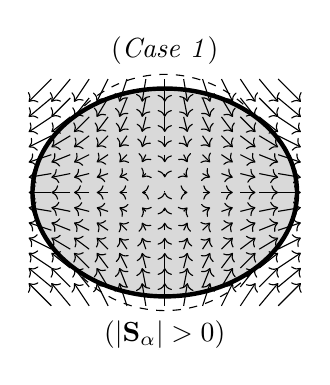
\begin{tikzpicture}[ultra thick,scale=0.6]
        \def\nRows{6}
        \def\nCols{6}
        \draw[dashed,thin] (0,0)circle(2.5);
        \draw[fill=gray!30] (0,0)ellipse(2.8 and 2.2);
        \foreach \x in {-\nRows,...,\nRows} {
            \foreach \y in {-\nCols,...,\nCols} {
                \pgfmathsetmacro\distance{veclen(\x*0.4, \y*0.4)};
                \pgfmathparse{\distance < 2.45 ? "blue" : "white"}
                \edef\colour{\pgfmathresult};
                \ifthenelse{\equal{\colour}{blue}}{                    
                    \draw[thin,->](\x*0.4,\y*0.4)--++(0.08*\x,-0.08*\y);
                }
            }
        }
        \node (txt) at (0,3){(\textit{Case 1})};
        \node (txt) at (0,-3){($|\textbf{S}_\alpha| > 0$)};
    \end{tikzpicture}
     \hfill
    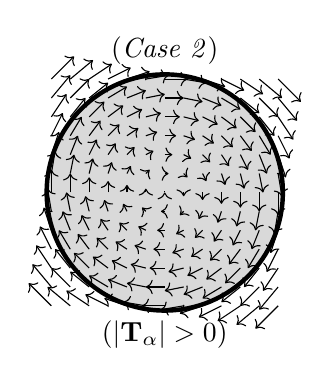
\begin{tikzpicture}[ultra thick,scale=0.6]
        \def\nRows{6}
        \def\nCols{6}
        \draw[fill=gray!30] (0,0)circle(2.5);
        \foreach \x in {-\nRows,...,\nRows} {
            \foreach \y in {-\nCols,...,\nCols} {
                \pgfmathsetmacro\distance{veclen(\x*0.4, \y*0.4)};
                \pgfmathparse{\distance < 2.5 ? "blue" : "white"}
                \edef\colour{\pgfmathresult};
                \ifthenelse{\equal{\colour}{blue}}{                    
                    \draw[thin,->](\x*0.4,\y*0.4)--++(0.08*\y,-0.08*\x);
                }
            }
        }
        \node (txt) at (0,3){(\textit{Case 2})};
        \node (txt) at (0,-3){($|\textbf{T}_\alpha| > 0$)};
    \end{tikzpicture}
    \hfill
    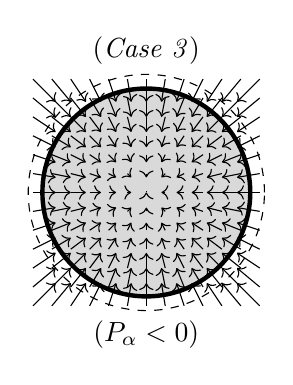
\begin{tikzpicture}[ultra thick,scale=0.6]
        \def\nRows{6}
        \def\nCols{6}
        \draw[dashed,thin] (0,0)circle(2.5);
        \draw[fill=gray!30] (0,0)circle(2.2);
        \foreach \x in {-\nRows,...,\nRows} {
            \foreach \y in {-\nCols,...,\nCols} {
                \pgfmathsetmacro\distance{veclen(\x*0.4, \y*0.4)};
                \pgfmathparse{\distance < 2.3 ? "blue" : "white"}
                \edef\colour{\pgfmathresult};
                \ifthenelse{\equal{\colour}{blue}}{                    
                    \draw[thin,->](\x*0.4,\y*0.4)--++(-0.08*\x,-0.08*\y);
                }
            }
        }
        \node (txt) at (0,3){(\textit{Case 3})};
        \node (txt) at (0,-3){($P_\alpha < 0$)};
    \end{tikzpicture}
    \hfill
    \caption{Graphical representation of the inner kinematics   of an arbitrary particle under three scenarios. 
        The arrows represent the velocity field inside the particle, $\textbf{w}_d^0$, with the corresponding value of the moment of momentum tensor indicated below. 
        The operator $|\ldots|$ refers to the norm of the tensors. 
        According to the inner velocity field:
        (\textit{Case 1}) The particle experiences a mean deformation, resulting in non-zero stretching of momentum along the principal axis of deformation;
        (\textit{Case 2}) The particle is rotating, leading to a non-zero angular momentum vector in the direction of rotation;
        (\textit{Case 3}) The particle undergoes compression, resulting in a negative trace of the moment of momentum.
    }
    \label{eq:scheme}
\end{figure}
Injecting, $f_d^0 = \rho_d$ in the second-order moment equation (derived in \ref{ap:Moments_equations}) we obtain,
%\JL{pq lequation du second moment de la masse ne fait pas intervenir la trace du premier moment de la qdm - cela semble incoherent ?}
\begin{equation}
    \ddt {\textbf{M}_\alpha}=2\textbf{S}_\alpha, %\JL{+2P_\alpha \bm\delta}, 
    \label{eq:dt_M_alpha}
\end{equation}
which is the second-order moment of mass conservation equation assuming that the fluid within the drop is divergence free. 
From \ref{eq:dt_M_alpha} we deduce that the evolution of the distribution of mass of a particle is solely determined by the stretching of momentum $\textbf{S}_\alpha$. 
This indicates that angular momentum does not influence the evolution of the second moment of mass, a consequence of the symmetry of the tensor $\textbf{M}_\alpha$, which must be preserved after differentiation with respect to time.
However, this does not imply that the particle angular velocity ($\bm\omega_\alpha$) does not appear in this equation. 
For instance, in the case of rigid body motion where $\textbf{w}_d^0 = \bm\omega_\alpha \times \textbf{r}$, we obtain the relation  $2\textbf{S}_\alpha = \bm\omega_\alpha \times \textbf{M}_\alpha+ \textbf{M}_\alpha\times \bm\omega_\alpha $. 
\JL{attention cette notation est bizarre : on fait un produit vectoriel entre un vecteur et un tenseur. l'ecrire sous forme indiciel ou faire reference a autre chose}
%Therefore, the angular velocity plays a significant role in the evolution of the second moment of mass equation. 

%\JL{ajouter lequation pour la derivee de $\textbf{S}_\alpha$ et discuter de celle pour la derivee seconde de $\textbf{M}_\alpha$}
Now that we have described the kinematics   of the particle shape, let us proceed to derive an equation for the moment of momentum.
This equation is derived by injecting $\textbf{Q}_\alpha^{(1)} = \textbf{P}_\alpha$ in \ref{eq:dt_Q_alpha_tot}, it reads, 
\begin{equation}
    \ddt {\textbf{P}_\alpha}
    - \intO{ \rho_d  \textbf{w}_d^0 \textbf{w}_d^0 }
    = 
    - \intO{\bm{\sigma}_d^0}
    - \intS{ 
        \gamma (\bm\delta - \textbf{nn})
    }
    + \intS{ \textbf{r}\bm{\sigma}_f^0\cdot \textbf{n}_d}.
    \label{eq:dt_P_alpha}
\end{equation}
The conservation equation of the angular momentum $\bm{\mu}_\alpha$ is obtained by taking the double contracted product of \ref{eq:dt_P_alpha} with $\bm\epsilon$, which directly gives
\begin{equation}
    \ddt\bm{\mu}_\alpha
    =  
    % \textbf{t}_\alpha.
    \intS{ \textbf{r} \times \bm{\sigma}_f^0\cdot \textbf{n}_d }
    \label{eq:dt_mu_alpha}
\end{equation}
Note that every term on the right-hand side of \ref{eq:dt_P_alpha} vanished due to their symmetric nature apart from the skew-symmetric part of the hydrodynamic stress, which is the hydrodynamic torque applied on the particle $\alpha$.
In particular, the surface tension terms do not appear in the angular momentum balance since the tensor $\bm\delta-\textbf{nn}$ is symmetric, which is consistent with the findings of \citet{hesla1993note}. 
As a consequence, the surface tension does not affect the angular momentum regardless of the particle shape. 
%In the literature, it is common to include the torque due to inter-particular interactions in the angular momentum balance, as is done in \citet{jackson1997locally} and \citet{zhang1997momentum}.
%In our case note that $\bm{\sigma}_f^0$ contains short-range hydrodynamic interaction forces. 

Taking the symmetric part of \ref{eq:dt_P_alpha}, and substrating the trace yields, 
\begin{align}
    &\ddt {\textbf{S}_\alpha}
    - \rho_d\intO{\left(\textbf{w}_d^0 \textbf{w}_d^0 -\frac{1}{3} (\textbf{w}_d^0 \cdot  \textbf{w}_d^0)\right)}
    = \nonumber \\
    &- 2\mu_d\intO{\textbf{e}_d^0}
    -  \intS{ \gamma
        \left( \frac{1}{3}\bm\delta - \textbf{nn} \right)
    }
    + \frac{1}{2}\intS{\left(\textbf{r}\bm\sigma_f^0+\bm\sigma_f^0\textbf{r}-\frac{2}{3}(\bm\sigma_f^0 \cdot \textbf{r})\bm\delta \right)\cdot \textbf{n}_d},
    \label{eq:dt_S_alpha}
\end{align}
%internal velocity kinetic energy. %$\intO{\rho_d\textbf{w}_d^0\textbf{w}_d^0 }$.
%On the left-hand side of \ref{eq:dt_S_alpha} we identify two inertial terms, i.e. the derivative of $\textbf{S}_\alpha$ and the stress induced by the product of internal velocity within the drop.
%The inertia of the particle is then balanced by the terms on the right-hand side of the equation, namely: 
%the volumic integral of the particle viscous stress; 
%the surface integral of the surface tension stress ; 
%and the first moment of the hydrodynamic stress tensor.
%A discussion regarding the physical implications of this equation is provided below. 
where we have introduced the rate of strain tensor for phase \( k \), defined as \( \mathbf{e}_k^0 = \frac{1}{2} (\nabla \mathbf{u}_k^0 + \nabla \mathbf{u}_k^0) \). 
On the left-hand side of Equation~\ref{eq:dt_S_alpha}, two inertial contributions can be identified: the time derivative of $\mathbf{S}_\alpha$, and the stress arising from the product of internal velocity field within the droplet. 
These inertial effects are counterbalanced by the terms appearing on the right-hand side of the equation, which include: the volume integral of the particle viscous stress; the surface tension moment; and the first moment of the hydrodynamic force.
%\JL{a finaliser}
While surface tension effects do not influence the linear or angular momentum equations directly, they do impact the moment of momentum $\textbf{P}_\alpha$, specifically its symmetric part $\textbf{S}_\alpha$.
Consequently, surface tension influences the hydrodynamic behavior of a particle exclusively through its effect on $\textbf{S}_\alpha$, which is related to the shape of a particle represented by $\textbf{M}_\alpha$, via \ref{eq:dt_M_alpha}.
%Whether it is solid or fluid particles \ref{eq:dt_S_alpha} becomes particularly relevant for expressing the averaged stress within an inertial suspension in terms of Lagrangian properties, as discussed in the next chapter. 
%\JL{enlever la trace}
%Taking the symmetric part of \ref{eq:dt_P_alpha}, and making use of \ref{eq:dt_M_alpha}, yields a dynamical balance equation for $\textbf{M}_\alpha$, namely
Inserting \ref{eq:dt_S_alpha} in  \ref{eq:dt_M_alpha} yields,
%\JL{enlever la trace et reecrire la partie ci-dessous + donner la definition de $e_d$ qui n'est pas de defini avant.}
\begin{align}    
    &\frac{1}{2}\frac{d^2 \textbf{M}_\alpha}{dt^2}
    =  \rho_d\intO{\left(\textbf{w}_d^0 \textbf{w}_d^0 -\frac{1}{3} (\textbf{w}_d^0 \cdot  \textbf{w}_d^0)\right)}
    - 2\mu_d\intO{\textbf{e}_d^0} \nonumber\\
    &- \intS{\gamma  
        \left( \frac{1}{3}\bm\delta - \textbf{nn} \right)
    }
    + \frac{1}{2}\intS{\left(\textbf{r}\bm\sigma_f^0+\bm\sigma_f^0\textbf{r}-\frac{2}{3}(\bm\sigma_f^0 \cdot \textbf{r})\bm\delta \right)\cdot \textbf{n}_d}.
    \label{eq:dt2_M_alpha}
\end{align}
%On the left-hand side of \ref{eq:dt_S_alpha}, we recover the symmetric part of the inertial contributions. 
%In opposition to \ref{eq:dt_P_alpha} we could substitute the term $\ddt (\textbf{P}_\alpha+\textbf{P}_\alpha^\dagger)$ initially present in the equation by $\ddt^2 \textbf{M}_\alpha$ using \ref{eq:dt_M_alpha}. 
%\ref{eq:dt2_M_alpha} is a second-order partial differential equation for the second order mass moment characterizing the droplet shape.
%In other words, \ref{eq:dt2_M_alpha} must be interpreted as an equation for the shape of the particle, represented by the tensor $\textbf{M}_\alpha$. 
%Thus, on the right-hand side of \ref{eq:dt_S_alpha}, we identify the terms which favors deformation, including the inertia of the velocity field within the droplet as well as the traceless part of the first moment and the terms wwohc resis deformation incluidng the viscous resistance within the droplet and the surface tension.
Equation \ref{eq:dt2_M_alpha} is a second-order differential equation governing the second-order mass moment that characterizes the droplet shape. 
In other words, it should be interpreted as an equation describing the droplet shape, represented by the tensor $\textbf{M}_\alpha$.
Accordingly, the right-hand side of \ref{eq:dt2_M_alpha} contains terms that promote deformation-such as the product of the internal velocity field and the traceless component of the first moment-as well as terms that oppose deformation, including droplet internal viscous resistance and surface tension.
%One might also recognize that \ref{eq:dt2_M_alpha} is in fact an extension of \citet{batchelor1970stress} result, but with the consideration of the inertia of the particle.
\ref{eq:dt2_M_alpha} is particularly useful to compute the unknown internal stress within solid particles, in terms of surface integral, i.e. the first moment of the hydrodynamic force.
This relation plays a key role in expressing the bulk stress of a suspension and ultimately leads to the effective viscosity, once a closed-form expression for the average first moment is obtained \citep{batchelor1970stress}. 
In the inertial regime, and for solid particles, the tensors $\textbf{M}_\alpha$ and the internal velocity field $\textbf{w}_d^0$ are fully prescribed by the particle kinematics. 
As a result, in equation \ref{eq:dt2_M_alpha}, $\textbf{M}_\alpha$ and $\textbf{w}_d^0$ appear not as unknowns but rather as known source terms.
For spherical particles specifically, the inertial correction to the first force moment has been derived by \citet{hwang1989modeling} and  \citet{lhuillier1996contribution}.
%For the specific case of spherical particles \citet{hwang1989,lhuillier1996contribution} have derived this inertial correction.
%This relation is used to express the bulk stress of a suspension.
%It eventually leads to the computation of the famous Einstein equivalent viscosity, upon having a closed expression for the average of the first moment \citep{guazzelli2011}. 
%In the inertial case and for solid particle, the tensors $\textbf{M}_\alpha$ and the inner velocity field $\textbf{w}_d^0$ are fully determined by the particle kinematic, indicating that $\textbf{M}_\alpha$ and $\textbf{w}_d^0$ can be used in \ref{eq:dt_S_alpha} not as unknowns but as source terms. 
%Consequently, for solid particles, \ref{eq:dt_S_alpha} must be interpreted as a generalized equation for the undefined stress $\bm\sigma_d^0$ integrated on the volume of the particles.

%Note that if intead we had considered spherical particles composed of compressible fluid \ref{eq:dt2_M_alpha} transforms into the Rayleigh-Lamb-Plesset equation as demonstrated in \citep{danielcours}.


%In our case, only the external contribution $\intS{\textbf{r}\bm\sigma_f^0\cdot \textbf{n}}$ is responsible for the generation of angular momentum, see \ref{eq:dt_mu_alpha}.
%Taking the symmetric part of this tensor ultimately removes this contribution. 

%\begin{equation}
%    \intO{\bm{\sigma}_d^0}
%    + \intS{\gamma(\bm\delta - \textbf{nn})}
%    = \frac{1}{2}\intS{(\textbf{r}\bm\sigma_f^0+\bm\sigma_f^0\textbf{r})\cdot \textbf{n}},
%    \label{eq:Batchelor}
%\end{equation}

%In \ref{ap:Moments_equations} we show how to derive the higher-order moment of momentum equations, which can also be viewed as formulas for the higher moments of the internal particle stress distribution. 
%It is interesting to mention that in a recent study of \citet{dolata2021faxen} and \citet{zhou2020lamb} they make use of the first two moments of momentum equations hidden into another but equivalent form, valid in the Stokes flow regime. 








\subsection{Averaged momentum and mass conservation equations}



Let us now focus on the averaged momentum equation of the continuous phase. 
By applying \eqref{eq:dt_f_k} with $f_k = \rho_f$ and $\rho_f\textbf{u}_f$ we obtain the mass and momentum equation for the continuous phase under the two fluid formulation, 
\begin{align}
    (\pddt + \textbf{u}_f\cdot \grad)\textbf{u}_f&=-\phi_f \div \textbf{u}_f
    \label{eq:mass_init}\\
    \phi_f \rho_f(\pddt + \textbf{u}_f  \cdot \grad) \textbf{u}_f
    % +  \div \avg{\chi_f\rho_f \textbf{u}_f'\textbf{u}_f'}
    &= 
    \div [\phi_f \bm\sigma_f-  \avg{\chi_f\rho_f \textbf{u}_f'\textbf{u}_f'}]
    + \phi_f \rho_f \textbf{g}
    - \avg{\delta_\Gamma \bm\sigma_f\cdot \textbf{n}}.
    \label{eq:two_fluid_momentum_init}
\end{align} 
To obtain the hybrid formulation one can expand the final term on the right-hand side of equation \ref{eq:two_fluid_momentum_init} using the Taylor expansion provided in \ref{eq:f_exp}.  
However, before doing so, it is important to examine the term \( \phi_f \bm\sigma_f \), as it contains a non-closed contribution originating from the averaging of the strain rate tensor. %a contribution from the dispersed phase. 
Properly identifying and isolating this contribution is a necessary step prior to performing the Taylor expansion.
%Moreover, there

%one may use \ref{eq:f_exp} to taylor expand the last term on the right-hand side of \ref{eq:two_fluid_momentum_init}. 
%However, it is first important to discuss the form of the term $\phi_f\bm\sigma_f$ since a dispersed phase term, is hidden into it, hence it is important to identify this term before carrying out the Taylor expansion. 

%\subsection{Mean stress formulation and momentum transfer decomposition}
%\JL{bien expliquer quand et comment apparaissent les distinctions sur le choix de la contrainte moyenne. en particulier voir en dessous}

We begin by noting that $\phi_f\bm\sigma_f$ can be expressed in terms of the averaged fluid pressure $p_f$, and continuous phase averaged velocity ($\textbf{u}_f$), or bulk-averaged velocity ($\textbf{u} = \phi_f \textbf{u}_f + \phi_d \textbf{u}_d$).
Expressing $\bm\sigma_f$ as a function of $\textbf{u}_f$ instead of $\textbf{u}$ (or vice versa) leads to two distinct forms of the momentum equation, each associated with different formulations of the closure terms. 
We also review several alternative choices found in the literature (see also \citet{jackson2000, pahtz2025general} for an overview focused on solid particles), emphasizing that while all these formulations are mathematically equivalent, they give rise to different closure problems. 
We argue that one particular formulation is probably the most suitable, especially in light of the closure terms available in the literature for non-dilute flows.%especially in the context of existing closure models for non-dilute flows.
%Choosing to express $\bm\sigma_f$ as a function $\textbf{u}_f$ rather than $\textbf{u}$ and vice versa, results in two distinct forms of the momentum equation and two distinct formulations of the closure terms. 
%We also discuss the various other choice available on the literature (see also \citet{jackson2000,pathz2025} for a review for solid particles) explaining that there is all choice are perfectly equivalent but leads to a different closure problems.
%Our belief his that there is one formulation which is the most appropriate with respect to of the closure terms available in the litterature for non-dilute flow.
%Although this topic has been already discussed in the context of solid particles  we propose here to expose both formulations and discuss which of the two equivalent (but different) formulations is the most suited for multiphase flow modeling. 

%Because we believe this topic has not been discussed much for non-solid particles in the literature, we propose here to expose both formulations and discuss which of the two equivalent (but different) formulation is the most suited for multiphase flow modeling. 
%Because we believe this topic has not been discussed much in the literature for non-solid particles, 

First we introduce what we refer to as the \textit{mean Newtonian stress}, based either on the continuous phase averaged velocity $\textbf{u}_f$ bulk velocity or on the \textbf{u}, namely,
\begin{align}
    \bm\Sigma_f 
    &
    = -p_f \bm\delta + 2\mu_f \textbf{E}_f    
    %= -p_f \bm\delta + \mu_f [\grad \textbf{u}_f + (\grad \textbf{u}_f)^{\dagger}], 
    \label{eq:Sigma_f_average}
    \\
    \bm\Sigma &
    = -p_f\bm\delta + 2 \mu_f \textbf{E}
    %= -p_f \bm\delta + \mu_f [\grad \textbf{u} + (\grad \textbf{u})^{\dagger}],
    \label{eq:Sigma_average}
\end{align}
where $\textbf{E}_f = [\grad \textbf{u}_f + (\grad \textbf{u}_f)^{\dagger}]/2$ and $\textbf{E} =[\grad \textbf{u} + (\grad \textbf{u})^{\dagger}]/2$ represent the \textit{mean strain rate} tensor based either on $\textbf{u}_f$ or on \textbf{u}. 
Additionally the ensemble averaged stress $\phi_f \bm\sigma_f$ may be written as 
\begin{equation}
    \phi_f \bm\sigma_f = - \phi _f p_f \bm\delta + 2 \mu_ f \phi_f \textbf{e}_f
    \label{eq:sigma_average}
\end{equation}
where $\phi _f \textbf{e}_f = \avg{\chi _f \textbf{e}_f^0}$. 
%Moreover by definition the bulk stress tensor reads $\textbf{E} = \phi _f\textbf{e}_f + \phi_d \textbf{e}_d$.
Inserting \ref{eq:Sigma_f_average} and \ref{eq:Sigma_average} in  \ref{eq:sigma_average} yields
%Using the constitutive law of Newtonian fluids we find, 
\begin{align}
    \phi_f \bm\sigma_f 
    &=
    % - \phi_f p_f \bm\delta
    % + \phi_f \mu_f [\grad \textbf{u}_f  + (\grad \textbf{u}_f)^\dagger]
    % - \mu_f \avg{\delta_\Gamma( \textbf{u}_f'  \textbf{n}_d +  \textbf{n}_d \textbf{u}_f' )}
    % =
    \phi_f \bm\Sigma_f
    - \mu_f \avg{\delta_\Gamma( \textbf{u}_f'  \textbf{n}_d +  \textbf{n}_d \textbf{u}_f' )}
    \label{eq:stress_closure}\\
    \phi_f \bm\sigma_f 
    &=
    % - \phi_f p_f \bm\delta
    % + \mu_f [\grad \textbf{u}  + (\grad \textbf{u})^\dagger]
    % - 2\mu_f \phi_d \textbf{e}_d
    % =
    \phi_f \bm\Sigma
    - \avg{2\mu_f \chi_d \textbf{e}_d^*}
    \label{eq:stress_closure1}
\end{align}
where we have used the relations 
\begin{equation}
    \avg{\chi_f \grad \textbf{u}_f^0}
    = 
    \phi_f \grad  \textbf{u}_f
    + \avg{\delta_\Gamma \textbf{n}_f \textbf{u}_f'}
    \label{eq:first_rel}
\end{equation}
and
\begin{equation}
    %\avg{\chi_f \textbf{e}_f^0}
%    = 
%    \avg{\textbf{e}^0}
%    - \avg{\chi_d \textbf{e}_d^0}
\phi _f\textbf{e}_f
%    = 
%    \textbf{E}
%    - \avg{\chi_d \textbf{e}_d^0}
    = 
    \phi_f \textbf{E}
    - \avg{\chi_d \textbf{e}_d^*},
    \label{eq:sec_rel}
\end{equation}
to derive \ref{eq:stress_closure,eq:stress_closure1}, respectively. 
 %in most practical situations of interest.
%Note that \ref{eq:first_rel} remains true in the presence of non zero interfacial rate of strain, while \ref{eq:sec_rel} requires the condition that the bulk rate of strain reads $\textbf{E} = \phi _f\textbf{e}_f + \phi_d \textbf{e}_d$ \textit{i.e.} that there is no shear stress at the interface of the droplets, so that $\avg{\delta_\Gamma \textbf{e}_\Gamma^0}= 0$, which is true in most of the practical cases of interest. 
In \ref{eq:stress_closure1} we have introduced $\textbf{e}_d^* = \textbf{e}_d^0 - \textbf{E} = \grad (\textbf{u}_d^0-\textbf{u})+\grad (\textbf{u}_d^0-\textbf{u})^\dagger$ which is the droplet internal shear rate relative to the `bulk' shear rate \textbf{E}.
%While $\textbf{u}_f' = \textbf{u}_f^0 - \textbf{u}_f$ in \ref{eq:stress_closure}. 
It is worth noting that equation \ref{eq:first_rel} remains valid even when the interfacial rate of strain is nonzero. 
In contrast, equation \ref{eq:sec_rel} holds under the assumption that the bulk rate of strain satisfies $\textbf{E} = \phi_f \textbf{e}_f + \phi_d \textbf{e}_d$, \textit{i.e.} that $\avg{\delta_\Gamma \textbf{e}_\Gamma^0} = 0$. 
This condition is supposed to be met here.
%Before presenting the hybrid form of the continuous phase momentum equation, it is interesting to expose the classic two-fluid formulation using the stress formulation given by \ref{eq:stress_closure} in the first place. 
%Before introducing the hybrid form of the continuous phase momentum equation, it is useful to first present the classical two-fluid formulation, employing the stress formulation \ref{eq:stress_closure}.
The averaged momentum equation  employing the stress formulation \ref{eq:stress_closure} read, 
\begin{align}
    % (\pddt + \textbf{u}_f\cdot \grad)\textbf{u}_f&=-\phi_f \div \textbf{u}_f\\
    \phi_f \rho_f(\pddt + \textbf{u}_f  \cdot \grad) \textbf{u}_f
    % +  \div \avg{\chi_f\rho_f \textbf{u}_f'\textbf{u}_f'}
    &= \phi_f 
    \left(\div \bm{\Sigma}_f
    + \rho_f \textbf{g}\right)
    - \div 
    [\avg{\chi_f\rho_f \textbf{u}_f'\textbf{u}_f'}
    +\avg{\delta_\Gamma \mu_f( \textbf{u}_f'  \textbf{n}_d +  \textbf{n}_d \textbf{u}_f')}]
    - \avg{\delta_\Gamma \bm\sigma_f^{(1)}\cdot \textbf{n}},
    \label{eq:two_fluid_momentum}
\end{align}
where, $\bm\sigma_f^{(1)}=\bm\sigma_f^0 - \bm\Sigma_f$ which also reads %is the Newtonian stress evaluated at a point on an interface relative to the mean stress $\bm\Sigma_f$. 
\begin{equation}
\bm\sigma_f^{(1)} = -p_f'\bm\delta
+ \mu_f [
    \grad \textbf{u}_f'
    + ^\dagger \grad \textbf{u}_f']
    \label{eq:disturbance_stress1}
\end{equation} 
Likewise, using \ref{eq:stress_closure1} one may also derive another form of the momentum equation, namely,
\begin{equation}
    \phi_f \rho_f(\pddt + \textbf{u}_f  \cdot \grad) \textbf{u}_f
    % +  \div \avg{\chi_f\rho_f \textbf{u}_f'\textbf{u}_f'}
    = \phi_f 
    \left(\div \bm{\Sigma}
    + \rho_f \textbf{g}\right)
    - \div 
    [\avg{\chi_f\rho_f \textbf{u}_f'\textbf{u}_f'} + \avg{2\mu_f \chi_d \textbf{e}_d^*}]
    - \avg{\delta_\Gamma \bm\sigma_f^{(2)}\cdot \textbf{n}},
    \label{eq:two_fluid_momentum2}
\end{equation} 
where $\bm\sigma_f^{(2)}=\bm\sigma_f^0 - \bm\Sigma$. 
%This stress tensor corresponds to the Newtonian stress (relative to the mean pressure and velocity field) typically available in numerical or theoretical studies. 
It can be also expressed as, 
%Clearly, subtracting by $\bm\Sigma_f$ to the local stress at the interface leads to the expression 
\begin{equation}
    \bm\sigma_f^{(2)} 
    =
    -p_f'\bm\delta
    + \mu_f [
        \grad \textbf{u}_f^*
        + ^\dagger \grad \textbf{u}_f^*
    ]
    \label{eq:disturbance_stress2}
\end{equation}
where $\textbf{u}_f^*= \textbf{u}_f^0 - \textbf{u}$.
%which corresponds to the Newtonian stress at the surface of the droplets (relative to the mean pressure and velocity field) typically available in numerical or theoretical studies.
%Likewise, substituting the mean stress with $\bm\Sigma$ in \ref{eq:disturbance_stress} one obtain the same formula except than $\textbf{u}_f'\to \textbf{u}_f^0 - \textbf{u}$. 
%Hence, 
In both cases (\ref{eq:two_fluid_momentum} and \ref{eq:two_fluid_momentum2}) one has to compute the local stress relative to the averaged continuous phase motion or bulk phase motion. 
% Note that because $\div \textbf{u} = 0$ it may be more convenient to  
%Note the differences between the last term of formulation \ref{eq:stress_closure} and \ref{eq:stress_closure1}, is equal to, $\phi_f (\div \bm\Sigma_f - \div\bm\Sigma)$
%Hence, the transition from one formulation to the other is straightforward, it just requires adding or subtracting $\phi_f (\div \bm\Sigma_f - \div\bm\Sigma)$. 
%However it is worth noting the physicsical meaning og this term which also reads,
Note the difference between the last terms in formulations \ref{eq:stress_closure} and \ref{eq:stress_closure1}, which is given by $\phi_f (\div \bm\Sigma_f - \div\bm\Sigma)$.
The transition from one formulation to the other is straightforward and only requires the addition or subtraction of this term. 
However, it is important to recognize its physical significance.
This difference can be expressed explicitly as,
\begin{equation}
    \phi_f (\div \bm\Sigma_f - \div\bm\Sigma) = \mu_f \phi_f \div \left(\grad (\phi _d \textbf{U}_r) + \grad (\phi _d \textbf{U}_r)^\dagger \right)
    \label{eq:diff_sigma1}
\end{equation}
%where $\textbf{u}_r = \textbf{u}_f - \textbf{u}_p$. 
%To derive this formula we make use of the relation $\textbf{u} = \phi_f \textbf{u}_f + \phi_d \textbf{u}_d$.
where $\textbf{U}_r = \textbf{u}_f - \textbf{u}_d$ is the phase averaged relative velocity between the fluid and dispersed phases, and the decomposition 
\begin{equation}
\textbf{u} = \phi_f \textbf{u}_f + \phi_d \textbf{u}_d,
\label{eq:u_mean} 
\end{equation}
has been used in the derivation.
Equation \ref{eq:diff_sigma1} reveals that the difference between the two formulations introduces a non-Newtonian stress term.
This non-Newtonian stress shares similarities with the second-order force moment closure \citep{jackson1997locally,zhang1997momentum}, and it typically related to intrinsic convection in sedimentation processes \citep{lhuillier2022}.
Therefore, when addressing the closure problem, it is essential to treat each stress formulation carefully, as the inclusion or exclusion of this additional term can significantly impact the resulting model.
%Then, when considering the colsure problem one has to be carefull to properly consider each formulation of the stress differently as both formulation will resulst in adding or removing this term.
%between \ref{eq:def_sigma_eff_f} and \ref{eq:def_sigma_eff_f2}  plus the differences between the corresponding drag force terms, is exactly equal to, $\phi_f (\div \bm\Sigma_f - \div\bm\Sigma)$.
%\JL{il faut que tu m'expliques : quand je soustrais les forces j'obtiens $\phi (\div \bm\Sigma_f - \div\bm\Sigma)$. OK on soustrait juste le RHS par ailleurs je pense qu'il faut detailler cela, c'est un point important.}
%\JL{en particulier $\div \bm\Sigma_f - \div\bm\Sigma = \div \nabla u_f - u \propto u_r$  a expliciter en montrant le developpment limite}





%Even though, both stress decomposition and momentum formulations proposed here are equivalent, each formulation have advantages and drawback which we discuss below.  
Although the stress decomposition and momentum formulations proposed herein are mathematically equivalent, each presents distinct advantages and limitations, which we examine in detail below.
%Now let us discuss on the choic between $\bm\Sigma$ and $\bm\Sigma_f$. 
%At first sight, using \ref{eq:dt_uf} with the effective stress given by \ref{eq:def_sigma_eff_f}, seems more practical because we are solving for the field $\textbf{u}_f$ hence avoiding the need of \ref{eq:velocity_conservation}. 
First, we may observe that a simplification arises for \ref{eq:stress_closure1} in the case of solid particles, for which $\textbf{e}_d^0 = 0$.
As a result $\phi _f \bm \sigma _f = - \phi _f p_f \bm\delta + 2 \mu_ f \textbf{E}$ \citep{joseph1990ensemble,jackson2000}. %and $\avg{\chi_d \textbf{e}_d^*} = -\phi_d\bm\Sigma$. \JL{a montrer}
Owing to this simplification, the formulation based on $\bm\Sigma$ and the associated closure relation \eqref{eq:stress_closure1} makes it a good candidate to be used in practice for solid particles. %is frequently adopted in the literature \citep{jackson2000}, despite requiring the inclusion of the additional momentum conservation equation.
Second, employing equation \ref{eq:two_fluid_momentum} with \ref{eq:disturbance_stress1} may appear more convenient as the governing equations are directly formulated in terms of the fluid velocity field $\textbf{u}_f$, thereby circumventing the need to explicitly include an expansion for the bulk fluid velocity. %the following equation
%Because $\textbf{u}$ may be required by \ref{eq:stress_closure1}, one also need to solve the equation, 
%\eqref{eq:velocity_conservation}.
%On the other hand we note that for solid particles $\textbf{e}_d^0 = 0$ and $\avg{\chi_d \textbf{e}_d'} = -\bm\Sigma\phi_d$, because of this great simplification \ref{eq:stress_closure1} is often used \citep{jackson2000} even if it requires adding \ref{eq:velocity_conservation} in the system of equation.  
%\JL{Je comprends l'interet de cette simplification, mais il faur toujours avoir une exression pr $\textbf{E}$ donc pour $\textbf{u}$}
Third, there exists a conceptual reason for preferring the bulk stress $\bm\Sigma$ when deriving closure relations for non-dilute suspensions.  %involving the fluctuating stress $\bm\sigma_f'$. 
Specifically, because $\bm\sigma_f^{(2)}$ depends on the disturbance velocity $\textbf{u}_f^* = \textbf{u}_f^0 - \textbf{u}$, the averaged velocity $\textbf{u}$ naturally serves as the "far-field" or "undisturbed" velocity boundary condition in the conditionally averaged Navier-Stokes equations \citep{hinch1977averaged,fintzi2025}. %(as also emphasized in the context of this PhD study).
%But there is another reason for using the `bulk stress' $\bm\Sigma$ as a reference stress to compute the closure terms involving $\bm\sigma_f'$. 
%Indeed, since $\bm\sigma_f'$ requires $\textbf{u}_f' = \textbf{u}_f^0 - \textbf{u}$, then \textbf{u} becomes the `far field' or `undisturbed' velocity boundary condition far from the test particle in the conditionally averaged Navier-Stokes equations \tb{(+my phd)}.
%On another hand, one may note that all the available theoretical solutions considering the disturbance field of a particle embedded in a pure solvent or in an effective medium (which represents other particles' contribution) use a divergence free `background flow' as limiting condition \citep{kim1985modelling,hinch1977averaged}.
%Since $\div \textbf{u} =0$ we deduce that the velocity field used in most (if not all) theoretical problems correspond to \textbf{u}. 
%Therefore, the disturbance  stress computed in these problems is $\bm\sigma_f'= \bm\sigma_f^0 - \bm\Sigma$. 
Notably, most (if not all) existing theoretical solutions addressing the disturbance field generated by a particle embedded in a Newtonian solvent or in an effective medium - representing other particles contribution - use a divergence-free background velocity field as limiting boundary condition \citep{hinch1977averaged, kim1985modelling}. 
Since $\nabla \cdot \textbf{u} = 0$, it follows that the velocity field used in these theoretical study corresponds to $\textbf{u}$. 
Consequently, the disturbance stress derived in those studies is $\bm\sigma_f^{(2)} = \bm\sigma_f^0 - \bm\Sigma$.
In opposition, the stress decomposition based on $\bm\Sigma_f$, involves the fields $\textbf{u}_f$ which is not divergence free. 
Hence, this `far field' or `undisturbed' velocity boundary condition far from the test particle does not correspond to the usual boundary condition assumed in most of the theoretical problems. 
%In conclusion, it is important to note that \textbf{u} corresponds exactly to the `background velocity' fields used in most of the theoretical derivations.
%Hence, the resulting closure terms (drag forces, stresslet and higher moments) derived in these studies refer to the closures expressed in terms of $\bm\sigma_f^0 - \bm\Sigma$.
%In all case one can always express $\bm\Sigma_f$ in terms of $\bm\Sigma$ hence which formulation to use is not a fatality. 
%However, one must always be careful when asserting that a given formulation of the drag force, for example, is exactly equivalent to a closure term found in the literature, as there are multiple possible formulations  (either based on $\bm\Sigma_f$, $\bm\Sigma$, $\bm\sigma_f$ or even  $p_f \bm\delta$). 
%Note that the choices between $\bm\Sigma_f$ and $\bm\Sigma$ only matter if one consider a closure problem, in which $\phi \textbf{u}_f \neq \phi \textbf{u}$, hence accurate at $\mathcal{O}(\phi^2)$ at least (such as in \citet{hinch1977averaged,kim1985modelling}). 
In conclusion, it is important to recognize that the vector field \(\textbf{u}\) corresponds precisely to the 'background velocity' typically employed in theoretical derivations. 
Consequently, the closure terms obtained in such analyses-such as drag forces, the stresslet, and higher-order moments-are formulated in terms of the difference \(\bm\sigma_f^0 - \bm\Sigma\).
However, it is always possible to express \(\bm\Sigma_f\) in terms of \(\bm\Sigma\) (see \ref{eq:diff_sigma1}), meaning that the choice of formulation remains free. 
Nevertheless, we must be cautious when claiming that a specific expression of, for example, the Faxen contribution to the force is exactly equivalent to a closure term reported in the literature especially for non-dilute suspension. 
%Multiple valid formulations exist, involving \(\bm\Sigma_f\), \(\bm\Sigma\), \(\bm\sigma_f\), or even the pressure tensor \(p_f \bm\delta\).
It should also be noted that the distinction between \(\bm\Sigma_f\) and \(\bm\Sigma\) becomes relevant only in the context of closure problems, particularly when \(\phi \textbf{u}_f \neq \phi \textbf{u}\), i.e., when effects at order \(\mathcal{O}(\phi^2)\) or higher are significant, as discussed in \citet{hinch1977averaged,kim1985modelling}.
\JL{pas compris cette derniere phrase que je pense il faut enlever : on montre que la distinction joue deja pour le second moment des forces en regime dilue non ?}

\JL{je n'ai pas compris le paragraphe suivant - je ne sais pas si il est necessaire desormais vu l'organisation actuelle ou on fait le developement en serie de Taylor plus tard}
% One can remark the similarities between the surface exchange terms expansion, and the multipole expansion used in microhydrodynamic that characterize the disturbance field caused by a body immersed in a stokes flow \citet{pozrikidis1992boundary,kim2013microhydrodynamics}. 
Moreover, one can wonder which of the formulation, \ref{eq:def_sigma_eff_f2} or \ref{eq:def_sigma_eff_f}, contains what is called the `Stresslet' and the higher moments of force given by the multipole expansion used in microhydrodynamic ? \citep{pozrikidis1992boundary,kim2013microhydrodynamics}\footnote{Note that the first term in this expansion is the same whether we use \ref{eq:def_sigma_eff_f2} or \ref{eq:def_sigma_eff_f}}.   
These moments are usually defined as the `extra stress above the value of the fluid law'\citep{hinch1977averaged}.
Because we are not studying the `bulk' momentum equation this definition does not directly apply in our context. 
However, note that \ref{eq:stress_closure1} involves the bulk velocity \textbf{u} which must be used in the bulk stress momentum equation.
Hence, we can state that the resulting formulation based on \ref{eq:stress_closure1} and given by \ref{eq:def_sigma_eff_f2}, corresponds to the multipole expansion of microhydrodynamic. 
\tb{not entirely sure but i think this is an important point }
Thus, the symmetric part of the second term of \ref{eq:def_sigma_eff_f2} is exactly what is called the `Stresslet', while the skew-symmetric part represents the hydrodynamic torque applied on the droplets.
The remaining terms of \ref{eq:def_sigma_eff_f2} represent the contribution of the second, third\ldots, and higher moments of hydrodynamic forces acted upon the droplets.  




%Additionally, because other stress decomposition have already been proposed in the literature we propose to discuss their advantages and draw back. 
%In the pioneering study of \citep{zhang1997momentum}, and in numerous articles that followed, the disturbance stress is defined as $\bm\sigma_f'= \bm\sigma_f^0 - \bm\sigma_f$ which is what we could call the ``intuitive'' definition. 
%However, note that using \ref{eq:stress_closure} one obtain that, 
Furthermore, given that various stress decomposition have already been introduced in the literature, we propose to examine their respective advantages and limitations. 
In the seminal work by \citet{zhang1997momentum}, as well as in numerous subsequent studies, the disturbance stress is defined as $\bm\sigma_f^{(3)} = \bm\sigma_f^0 - \bm\sigma_f$, a formulation that may be regarded as the "intuitive" definition. 
However, it is important to note that, by employing Equation~\ref{eq:stress_closure}, one obtains
\begin{equation}
    \bm\sigma_f^{(3)}
    = \bm \sigma _f ^{(1)}
%    -p_f'\bm\delta
%    + \mu_f [
%        \grad \textbf{u}_f'
%        + ^\dagger \grad \textbf{u}_f'
%    ]
    + \frac{\mu_f}{\phi_f} \avg{\delta_\Gamma( \textbf{u}_f'  \textbf{n}_d +  \textbf{n}_d \textbf{u}_f' )}
    \label{eq:stress_closure_zhang}
\end{equation}
%The first term on the rhight hand side of this expression correspond to the relative Newtonian stress usually integrated on the surface of a droplet or solid particle.
%The last term is a contribution related to the stress induced by the dispersed phase which normally appear in the effective stress expansion as shown below.
%To provide a better understanding of this term we assume that the suspension is made of solid particles $\textbf{e}_d = 0$.%for the following discussion 
The last term represents a contribution from the stress induced by the dispersed phase, as illustrated below. 
To better understand this term, we consider the case of a suspension composed of rigid solid particles, for which the strain rate tensor of the dispersed phase vanishes, i.e., $\textbf{e}_d = 0$.
%we remark that for solid particles . 
By subtracting \ref{eq:stress_closure} from \ref{eq:stress_closure1}, we directly obtain
\begin{equation}
    \avg{\delta_\Gamma (\textbf{n}_d \textbf{u}_f'+  \textbf{u}_f' \textbf{n}_d)}
    = 2 \mu _f \phi _f (\textbf{E}_f - \textbf{e} _f).
\end{equation} 
Since for solid particles $\textbf{e} _f = \textbf{E}/\phi _f$ we obtain,
\begin{equation}
    \avg{\delta_\Gamma (\textbf{n}_d \textbf{u}_f'+  \textbf{u}_f' \textbf{n}_d)} = 
    \textbf{U}_r\grad \phi_d + \grad \phi_d \textbf{U}_r   
%(\textbf{u}_f - \textbf{u}_d)\grad \phi_d + \grad \phi_d (\textbf{u}_f - \textbf{u}_d)
-  \phi_d [\grad \textbf{u}_d+ (\grad \textbf{u}_d)^\dagger ]. 
\label{eq:closure_un_nu}
\end{equation} 
where we have used \ref{eq:u_mean}.
Therefore, at least in the case of solid particles, this term becomes non-zero whenever there are significant gradients in volume fraction and mean particle velocity, as in the recent study by \citet{wang2024effect}.
%Therefore, at least for solid particles, this term is non-zero as soon as there are non-negligible gradients of volume fraction and mean gradients of particle velocities as in the recent work of \citet{wang2024effect}. 
%This finding implies that, in the recent work of \citet{wang2024effect}, where decomposition is employed for the drag force, we assert that they have actually computed the integral of the first two terms of \ref{eq:sigma_explict}, while neglecting the final term. 
%We conclude that the commonly used decomposition of the drag force introduced by \citet{zhang1997momentum,jackson2000}, given by \ref{eq:general_partition}, requires adding the term  $\avg{\delta_\Gamma (\textbf{n}_d \textbf{u}_f'+  \textbf{u}_f' \textbf{n}_d)}$ to the classical Newtonian stresses in the second term of \ref{eq:general_partition} and subtracting it in the mean drag force term (first term of \ref{eq:general_partition}). 
%Interestingly, \citet{wang2024effect}\footnote{
%    In this study the drag force is defined as the second term on the right-hand side of \ref{eq:drag_final} (see equation (3) of \citet{wang2024effect}).
%    They compute the drag force term using DNS by integrating $\bm\sigma_f^0$ over the particles surfaces, hence, assuming that $\bm\sigma_f=0$ (because there is no mean pressure gradient or velocity gradient).  
%    However, it is likely that the author overlooked the last term of \ref{eq:sigma_explict} which is non-zero \eqref{eq:closure_un_nu} in this specific scenario because $\grad \phi_d \neq 0$. 
%} specifically investigates the effect of the volume fraction gradient ($\grad \phi_d$) on the drag force. 
%\JL{a finaliser, rederiver la relation de Nico}
%Same comments apply if one consider \ref{eq:stress_closure1} in the above expression. 
%Hence, because $\bm\sigma_f$ already contains closure terms related to the dispersed phase, it appears to be prone to error to subtract the whole expression of $\bm\sigma_f$ from $\bm\sigma_f^0$.
The same observations hold if one considers expression \ref{eq:stress_closure1} in the analysis above. 
Since $\bm\sigma_f$ already includes closure contributions associated with the dispersed phase, directly subtracting the full expression of $\bm\sigma_f$ from $\bm\sigma_f^0$ can lead to inconsistencies unless the closure problem is handled with sufficient care.%if sufficient care is not done in the closure problem.
Nevertheless, note that because the last term of \ref{eq:stress_closure_zhang} is at most of $\mathcal{O}(\phi)$, the total contribution from this term when integrated on the droplets surface becomes of $\mathcal{O}(\phi^2)$, hence it can be safely neglected in dilute regime. 
\JL{pas compris cette derniere phrase.}

Another commonly adopted approach in the literature is $\bm \sigma ^{(4)} = \bm \sigma _f ^0 - p_f\bm\delta$ \citep{simonin1996,lhuillier2009rheology,morel2015mathematical,guazzelli2018rheology}.
This definition leads to the expression
\begin{equation}
    \bm\sigma_f^{(4)}  = -p_f' \bm\delta + \mu_f (\grad \textbf{u}_f^0 + ^\dagger \grad \textbf{u}_f^0),
\end{equation}
which implies that the closure is based on the absolute local fluid velocity $\textbf{u}_f^0$, rather than the fluctuating component $\textbf{u}_f'$.
%Hence the closure are computed based on the absolute local velocity $\textbf{u}_f^0$ instead of $\textbf{u}_f'.
%or in the case with buoyant particles simply $\sigma ^{(4)} = \bm \sigma _f ^0 - \rho_f\bm\delta$ \citep{lhuillier}
%One may also consider using  instead of $\bm\sigma_f$, $\bm\Sigma_f$ or $\bm\Sigma$, as done in \citet{morel2015mathematical} (\tb{paper de daniel ou il fait ca ?}), in this case $\bm\sigma_f'  = -p_f' \bm\delta + \mu_f (\grad \textbf{u}_f^0 + ^\dagger \grad \textbf{u}_f^0)$, hence the closure are computed based on the absolute local velocity $\textbf{u}_f^0$ instead of $\textbf{u}_f'$.
Without going into the details, note that numerous closures are based on the reciprocal theorem formulation \citep{kim2013microhydrodynamics,stone2001inertial,raja2010inertial}.%, this includes the Faxen contribution to the drag force . %the expressions given by the famous Faxen laws.
The closures (drag forces, stresslet etc... ) provided by the reciprocal theorem are by construction expressed in terms of the disturbance fields ($p_f'$,$\textbf{u}_f'$), because they must decay to zero far from the test particle. 
%Therefore, this last formulation may not be the most practical as well\footnote{
For example, the Faxen contribution to the drag force in the case of a spherical solid particle of radius $a$ is given by $\textbf{f} = \pi a^3 \mu_f \grad^2 \textbf{u}_f$. 
This formulation is obtained  by considering the contribution from the disturbance stress, $\bm\sigma ^{(1)}  = -p_f' \bm\delta + \mu_f (\grad \textbf{u}_f' + ^\dagger \grad \textbf{u}_f')$, which vanish far from the test particle. 
If one uses the formulation based on $\bm\sigma_f^{(4)}  = -p_f' \bm\delta + \mu_f (\grad \textbf{u}_f^0 + ^\dagger \grad \textbf{u}_f^0)$, the Faxen contribution to the drag force becomes $\textbf{f} = \pi a^3 \mu_f \grad^2 \textbf{u}_f + \frac{4\pi a^3}{3}\mu_f \grad^2 \textbf{u}_f$ where the second term is the contribution from the mean velocity field.
Although both formulations are equally valid, the second one appears to be less commonly used and could potentially lead to misinterpretations or inconsistencies if not carefully handled. 
%}. 


\JL{ajouter a la discussion le choix de Jackson et Pahtz si tu le souhaites mais moi j'ai la flemme}

%Because of those remarks, we will use in the following the formulation based on $\bm \sigma^{(2)}$ i.e. \ref{eq:two_fluid_momentum2} since we believe this is a formulation less prone to errors when considering the closure problem. 
%Moreover this is the formulation used in the closure problem for non-dilute flows. 
%For simplicity we will denote $\bm \sigma^{(2)} = \bm \sigma ^{*}$ in the rest of the paper.
%since we are working at $\mathcal{O}(\phi)$.
In light of these considerations, we adopt the formulation based on $\bm \sigma^{(2)}$-i.e., Equation \ref{eq:two_fluid_momentum2}-for the remainder of this work, as it is less prone to errors when considering the closure problem. 
Furthermore, this formulation is commonly employed in the analysis of non-dilute flows. 
For simplicity, we will denote $\bm \sigma^{(2)}$ as $\bm \sigma^{*}$ throughout the rest of the paper.
%This will avoid the need for \ref{eq:velocity_conservation} in the system of equation. 
%\tb{on pourrait utiliser aussi lautre peut importe }
%\JL{finaliser la discussion sur le fait que $\Sigma$ est le moins prine to errors + more ealsily extendeable to non dilute fraction}
%The last two terms on the right-hand side of \ref{eq:two_fluid_momentum} can be further expanded into a Taylor series using \ref{eq:f_exp_delta}. 
%Doing so leads us to the hybrid formulation of the continuous phase momentum  equation %(i.e. \ref{eq:avg_hybrid_dt_chi_f} %with $f_f^0 = \textbf{u}_f^0\rho_f$), namely,
%This gives the hybrid formulation of the continuous phase momentum equation,
%\begin{align}
%    \phi_f \rho_f(\pddt + \textbf{u}_f  \cdot \grad) \textbf{u}_f
%    &= \phi_f 
%    \left(\div \bm{\Sigma}_f
%    + \rho_f \textbf{g}\right)
%    + \div \bm\sigma_f^{(1)\text{eff}}
%    - \pSavg{\bm\sigma_f^{(1)}\cdot \textbf{n}}, 
%    \label{eq:dt_uf}
%\end{align}
%where we introduced the effective stress, 
%\begin{align}
%    \bm{\sigma}^{(1)\text{eff}}_f 
%    &= 
%    - \avg{\chi_f\rho_f \textbf{u}_f'\textbf{u}_f'} 
%    + \pSavg{[\textbf{r}\bm\sigma^{(1)}_f\cdot \textbf{n} - \mu_f (\textbf{u}_f' \textbf{n} + \textbf{n} \textbf{u}_f')]}\nonumber\\
%    &- \div
%        \pSavg{[\frac{1}{2}\textbf{rr}\bm\sigma^{(1)}_f\cdot \textbf{n}- \mu_f\textbf{r} (\textbf{u}_f' \textbf{n} + \textbf{n} \textbf{u}_f')]}
%        + \grad\grad (\ldots)
%    \label{eq:def_sigma_eff_f}
%\end{align}
%\JL{a finaliser}
The last two terms on the right-hand side of \ref{eq:two_fluid_momentum2} can be further expanded into a Taylor series using \ref{eq:f_exp_delta}.
Doing so leads us to the hybrid formulation of the continuous phase momentum  equation, %a relation similar to \ref{eq:dt_uf} except that $\bm\Sigma_f$ is replaced by $\bm\Sigma$, $\pSavg{\bm\sigma_f^{(1)}\cdot \textbf{n}}$ by $\pSavg{\bm\sigma_f^{(2)}\cdot \textbf{n}}$ and the effective stress $\bm\sigma_f^\text{(1)eff}$ by the tensor
\begin{align}
    \phi_f \rho_f(\pddt + \textbf{u}_f  \cdot \grad) \textbf{u}_f
    &= \phi_f 
    \left(\div \bm{\Sigma}
    + \rho_f \textbf{g}\right)
    + \div \bm\sigma_f^{\text{eff}}
    - \pSavg{\bm\sigma_f^{*}\cdot \textbf{n}}, 
    \label{eq:dt_uf2}
\end{align}
where,
\begin{align}
    \bm{\sigma}^{\text{eff}} 
    &= 
    - \avg{\chi_f\rho_f \textbf{u}_f'\textbf{u}_f'} 
    + \pavg{\intO{\textbf{r}\bm\sigma^{*}_f\cdot \textbf{n}} - \delta_p\intO{2\mu_f\textbf{e}_d^*}}\nonumber\\
    &- \div
        \pavg{ \frac{1}{2}\intS{\textbf{rr}\bm\sigma^{*}_f\cdot \textbf{n}}
        - \delta_p\intO{2\mu_f \textbf{r} \textbf{e}_d^*}}
        + \grad\grad (\ldots). 
    \label{eq:def_sigma_eff_f2}
\end{align}
Under these forms, the left-hand side of \ref{eq:dt_uf2} represents the total derivative of $\textbf{u}_f$, while on the right-hand side we find: (1) the mean Newtonian stress contribution based on the bulk velocity $\bm\Sigma$, (2) the mean buoyancy force, (3) the Reynolds stress term, and (4) the moments of momentum exchange terms, which are computed based on $\bm\Sigma$. 
The last term correspond to the mean hydrodynamic drag force on the particles.
%\JL{il faut mettre les closure pr connaitre les ordres de grandeurs.}
%In this formulation it is implied that $\bm\sigma_f'$ is given by $\bm\sigma_f' = \bm\sigma_f^0 -\bm\Sigma$.

The mean mass ($m_p$), the mean center of mass velocity ($\textbf{u}_p$), the mean second moment of mass ($\textbf{M}_p$), and the mean first moment of momentum ($\textbf{P}_p$), are defined as,
\begin{align}
    n_p m_p 
    =
    \pOavg{\rho_d},
    && n_p m_p \textbf{u}_p  
    =
    \pOavg{\rho_d \textbf{u}_d^0}\\
    n_p \textbf{M}_p  
    =
    \pOavg{\rho_d \textbf{rr} },
    && n_p \textbf{P}_p  
    =
    \pOavg{\rho_d \textbf{r} \textbf{u}_d^0},
\end{align} 
respectively.
All the quantities defined above obey conservation laws that are given according to \ref{eq:avg_hybrid_q}, \ref{eq:avg_hybrid_q_1} and \ref{eq:avg_hybrid_q_n} (for conservation laws at the local scale, refer to the previous section.).
They read, 
%\JL{pq lequation du second moment de la masse ne fait pas intervenir la trace du premier moment de la qdm - cela semble incoherent ? OK car on est en incompressible}
%\JL{attention il manque des primes sur certaines variables}
\begin{align}
    (\pddt + \textbf{u}_p \cdot \grad)n_p
    &=
    - n_p \div \textbf{u}_p\label{eq:mass_p}\\
    n_p (\pddt + \textbf{u}_p \cdot \grad) \textbf{M}_p
    +\div  \pavg{\textbf{u}_\alpha'\textbf{M}_\alpha}
    &=
    n_p2  \textbf{S}_p
    \label{eq:dt_hybrid_Mp}\\
    \label{eq:dt_hybrid_up}
    m_p n_p(\pddt + \textbf{u}_p \cdot \grad)\textbf{u}_p
    + \div \pavg{m_p \textbf{u}_\alpha'\textbf{u}_\alpha'}
    &=
    m_p n_p \textbf{g}
    %+ \pSavg{\bm\sigma_f^0 \cdot \textbf{n}}\\
    + \pSavg{\bm\sigma_f^* \cdot \textbf{n}} + \pSavg{\bm\Sigma \cdot \textbf{n}}\\
    \label{eq:dt_hybrid_mup}
    n_p (\pddt + \textbf{u}_p \cdot \grad) \bm{\mu}_p
    +\div  \pavg{\textbf{u}_\alpha'\bm\mu_\alpha}
    &=
    \pSavg{\textbf{r}\times(\bm\sigma_f^*\cdot \textbf{n}_d)}
    \\
    \label{eq:dt_hybrid_Sp}
    \color{red}
    n_p (\pddt + \textbf{u}_p \cdot \grad) \textbf{S}_p
    +\div  \pavg{\textbf{u}_\alpha'\textbf{S}_\alpha}
    &=
    \rho_d \pOavg{
        \textbf{w}_d^0  \textbf{w}_d^0 
        -\frac{1}{3} (\textbf{w}_d^0 \cdot  \textbf{w}_d^0) \bm\delta
    }
    -2 \mu_d \pOavg{\textbf{e}_d^*} \nonumber \\
    &+\pSavg{\frac{1}{2}(\textbf{r}\bm\sigma_f^*+\bm\sigma_f^*\textbf{r}-\frac{2}{3}(\bm\sigma_f^* \cdot \textbf{r})\bm\delta)\cdot \textbf{n}_d}\nonumber\\
    &-  \pSavg{\gamma (\frac{1}{3}\bm\delta - \textbf{nn})}
     + (1-\lambda)\pOavg{2\mu_f\textbf{E}}\\
     &+ \frac{1}{2}\pOavg{\textbf{r}(\div\bm\Sigma)+ (\div\bm\Sigma) \textbf{r}},
\end{align}
\JL{j'ai mis la derniere equation en rouge car n'arrivant pas à la demontrer je ne suis pas sur du second membre. par ailleurs il y avait des petites coquilles dans les autres équations que j'ai corrigé. je te laisse regarder si jamais tu en vois d'autres}
%\JL{discuter du lien avec Curtiss (equations pour les particules non spheriques). en particlier ne ne pense pas que lequation de $S_p$ soit necessaire}
%The above system of equations is a generalization of the averaged equations for non-spherical particles \citep{curtiss1956kinetic}. 
%One may note that for solid particles \ref{eq:dt_hybrid_Sp} is useless as $\textbf{S}_p$ can be expressed  as a function of $\textbf{M}_p$ and $\bm{\mu}_p$ and correlation between their fluctutations. 
where $\textbf{S}_p$ is the mean symmetric traceless part of $\textbf{P}_p $ and $\mu_p$ the mean angular momentum.% have respectively 
The presented system of equations extends the averaged equations developed for non-spherical solid particles \citep{curtiss1956kinetic}. 
It is worth noting that, in the case of solid particles, equation \ref{eq:dt_hybrid_Sp} becomes redundant, as the tensor $\textbf{S}_p$ can be expressed in terms of $\textbf{M}_p$, $\bm{\mu}_p$ or the mean angular velocity, and the correlations of their fluctuations.
%In these equations we have introduced the rate of strain tensor $\textbf{e}_k^0 = 1/2 (\grad \textbf{u}_k^0 + \grad \textbf{u}_k^0)$. %as the local shear rate of phase $k$.
%It is now clear that if the surface tension forces play no role in the linear and angular momentum equation, however, it impacts the moment of momentum $\textbf{P}_\alpha$ or more specifically its symmetric part $\textbf{S}_\alpha$.
%Thus, the surface tension force impacts the hydrodynamic behavior of a particle solely through its action on $\textbf{S}_\alpha$, which is related to the shape of a particle represented by $\textbf{M}_\alpha$, through \ref{eq:dt_M_alpha}.
%In \ref{ap:Moments_equations} we show how to derive the higher-order moment of momentum equations, which can also be viewed as formulas for the higher moments of the internal particle stress distribution. 
%It is interesting to mention that in a recent study of \citet{dolata2021faxen} and \citet{zhou2020lamb} they make use of the first two moments of momentum equations hidden into another but equivalent form, valid in the Stokes flow regime. 
%Although surface tension effects do not directly influence the linear or angular momentum equations, they impact the moment of momentum \( \mathbf{P}_\alpha \), and more specifically, its symmetric component \( \mathbf{S}_\alpha \).
%Consequently, the impact of surface tension on the hydrodynamic behavior of a particle manifests exclusively through its contribution to \( \mathbf{S}_\alpha \). 
%This quantity is related to the particle shape, represented by \( \mathbf{M}_\alpha \), via equation \ref{eq:dt_M_alpha}.
In Appendix \ref{ap:Moments_equations}, we detail the derivation of higher-order moment of momentum equations, which can also be interpreted as expressions for the higher moments of particles internal stress distribution. 
Notably, recent works by \citet{dolata2021faxen} and \citet{zhou2020lamb} have employed the first two moment equations in an alternative but equivalent form, valid in the Stokes flow regime.
\JL{pas compris la comparaison avec les travaux de Dolata et Zhou qui pour moi considerent les moments des forces ?}
% In these expressions we partitioned the local hydrodynamic stress $\bm\sigma_f^0$ and $\bm\sigma_d^0$, into their fluctuating parts, $\bm\sigma_f'=\bm\sigma_f^0 - \bm\Sigma_f$,  $\bm\sigma_d' = \bm\sigma_d^0 + p_f\bm\delta - 2\mu_d \textbf{E}_f$ and mean parts $\bm\Sigma_f$ and $-p_f \bm\delta + 2\mu_d \textbf{E}_f$, respectively. 
% Note that one can also write these equations in terms of $\bm\Sigma$ and $\textbf{E}$, the only requirement being that the exchange terms of \ref{eq:dt_hybrid_Mp} to \ref{eq:dt_hybrid_Sp} must correspond to the exchange terms used in the continuous phase momentum conservation \eqref{eq:dt_uf} (with \ref{eq:def_sigma_eff_f} or \ref{eq:def_sigma_eff_f2}). 

The set of equations \ref{eq:mass_init}, \ref{eq:dt_uf2}, \ref{eq:mass_p}-\ref{eq:dt_hybrid_Sp} are completed by the following relations%condition on the total volume conservation which reads, 
\begin{align}
    \phi_f + \phi_d &= 
    \phi_f +  n_pv_p + \frac{1}{2}\grad\grad : (\textbf{M}_p n_p) + \ldots = 1,
    \label{eq:volume_conservation}\\
    \textbf{u} &= \textbf{u}_f\phi_f + 
    n_pv_p\textbf{u}_p - \frac{1}{\rho_d} \div  (\textbf{P}_p n_p) + \ldots
    \label{eq:velocity_conservation}
\end{align}
The latter is obtained by inserting expansion \ref{eq:f_exp_chi} in \ref{eq:u_mean}.

\subsection{Symmetry of the effective stress tensor}
%\JL{specifier que l'on parle bien des contraintes eqs cote fluide.}
We remark that the second moment and higher-order moments in \ref{eq:def_sigma_eff_f2} appear under two divergence operators in \ref{eq:dt_uf2}. 
Hence, if we note $\Sigma_{ijk}$ the third rank tensor that represent these moments, then only the vector $\partial_k \partial_j\Sigma_{ijk}$ is of physical significance in the momentum balance \eqref{eq:def_sigma_eff_f}.
Thus, one can demonstrate that \citep{lhuillier1996contribution}
\begin{equation}
    \partial_j \partial_k \Sigma_{ijk}
    = \partial_j \partial_k \Sigma_{i(jk)}
    =
    \partial_j \partial_k \left[
        \Sigma_{i(jk)}
        + \Sigma_{j(ik)}
        - \Sigma_{k(ij)}
    \right],
    \label{eq:sym_proof}
\end{equation}
where $\Sigma_{i(jk)} = \frac{1}{2}[\Sigma_{ijk} + \Sigma_{ikj}]$ represents the symmetric part of $\Sigma_{ijk}$ over the index $jk$, as indicated by the parenthesis (and so on for the other tensor). 
This expression is allowed because $\partial_j \partial_k (\Sigma_{ijk} - \Sigma_{ikj}) = 0$ and $\partial_j \partial_k (\Sigma_{j(ik)} - \Sigma_{k(ij)}) = 0$. 
This manipulation highlight the fact that the effective stress due to the second order moments remains symmetric over the indices $ij$, in all circumstances.
Hence, as already demonstrated by \citet{lhuillier1996contribution} only the hydrodynamic torque can induce skew-symmetric stresses in \ref{eq:dt_uf}. 
\JL{je ne comprends pas pq on regarde directement la symetrie du second moment et pas ceux d'avant ?}

\tb{verifier le papier de Daniel}



\section{Closure for dilute suspensions of droplets in viscous dominated flows}
We now consider the closures for a dilute, monodisperse suspension of spherical droplets with radius \( a \) in Stokes flow.%, in the absence of mass transfer. 
%We then examine the closure problem for dilute monodisperse droplets in Stokes flow. 
Our analysis recovers the results of \citet[Appendix B]{zhang1997momentum}. 
We extend these results by considering the first moment of momentum for the dispersed phase accounting for the angular momentum. 
We demonstrate how higher-order moments can characterise droplet shapes and relate them to the averaged equations governing the continuous phase. 
%\JL{Finally, we derive expressions for the third-order force moments and consider closures that incorporate finite inertia effects.}
%We also discuss the closure of the various terms appearing in the averaged equations.
%Finally we discuss the effects of Marangoni effects on the dynamics of the suspension.
We also address the closure of the various covariance terms arising in the averaged equations.
Finally, we examine the influence of Marangoni effects on the suspension dynamics.
%\subsection{Closure in viscous dominated flows for dilute suspension}
\subsection{Hydrodynamic stresses closures at $\mathcal{O}(\phi Ca)$ and $\mathcal{O}(\phi Re )$}
\JL{reformuler le debut de cette partie pour bien expliquer les parametres sans dimension et l'expansion en $a/L$}
In the averaged equations, we neglect droplet inertia, thereby discarding all terms of order $\mathcal{O}(Re \phi)$. 
Additionally, we assume the droplets are spherical, which allows us to neglect terms of order $\mathcal{O}(\phi Ca)$. 
The Reynolds number ($Re$) and Capillary number ($Ca$) are defined in \ref{tab:qte_Newtonian}.
\begin{table}
    \centering
\begin{tabular}{|c|c|}\hline
    Velocity scale & $U$ \\
    Macroscopic length scale & $L$ \\
    Droplets radius & $a$ \\
    Reynolds number & $Re = \rho_f a U / \mu_f$   \\
Capillary number & $Ca = \mu_f U / \gamma$ \\\hline
Viscosity ratio & $\lambda = \mu_d / \mu_f$ \\
Density ratio & $\zeta = \rho_d / \rho_f$ \\
\hline
    \end{tabular}
    \caption{Definition of Physical Quantities and Dimensionless Parameters.
    Note that the choice of velocity scales depends on the specific problem under consideration. 
    For example, in the case of purely sedimenting droplets, the characteristic velocity is typically $U \sim |\textbf{u}_p|$.}
        %Definition of the physical quantities and dimensionless parameters. 
    %Note that the velocity scales depend of the problem of interest. 
    %For instance for purely sedimenting droplets $U\sim |\textbf{u}_p|$.} %or $\mathcal{O}(|\textbf{u}_f - \textbf{u}_p|)}
\end{table}

The closure terms in the above set of equation are expressed in terms of $p_f'$ and $\textbf{u}_f'$, therefore we are seeking for the disturbance velocity and pressure fields generated by a spherical droplet immersed in an arbitrary flow. 
Specifically, the fields $(\textbf{u}_f',p_f')$ correspond to the solution of the 
 \textit{single-particle conditionally averaged} Navier-Stokes equations \citep{hinch1977averaged,zhang1994averaged,fintzi2025}. 
Note that to obtain a solution accurate at $\mathcal{O}(\phi)$ to these equations, it is sufficient to consider a closure problem accurate at $\mathcal{O}(\phi)$\citep{hinch1977averaged,zhang1994averaged}.
Additionally, we neglect inertia in the closure problem, meaning that we neglect all the terms of $\mathcal{O}(Re)$ in the closure problem, and all the term of $\mathcal{O}(Re\phi)$ in the averaged equations. 
Finally in at first we disregard any Marangoni effects and consider the surface tension to be constant.
Consequently, we consider an isolated spherical droplet translating in an arbitrary Stokes flow.
The solution for this problem can be found in many studies in the literature, including \citet{leal2007advanced,pozrikidis1992boundary,kim2013microhydrodynamics,pozrikidis2011introduction,nadim1991motion} which will enable us to compute the closure terms.

%\subsubsection{Hydrodynamic stresses closures at $\mathcal{O}(\phi Re^0 Ca^0)$}
%\JL{pq la partie antisymetrique du premier moment est nulle ?}
In the first place we focus on the surface exchange terms. 
We may directly compute the following expressions from the singularity solutions and find, 
\begin{align}
    \pSavg{\bm\sigma_f^*\cdot \textbf{n}} &
    =
    \phi
    \frac{\mu_f}{a^2}
    \frac{3(2+3\lambda)}{2(1+\lambda)}\textbf{u}_r
    + \phi\mu_f  \frac{3\lambda}{4(\lambda +1)} \grad^2 \textbf{u}_f\\
    + \phi \frac{1}{a}\frac{1}{\lambda +1} \grad \gamma
    + \phi a \frac{1}{10(\lambda +1)}\grad^2(\grad\gamma)
    \label{eq:drag_forces}
    \\
    \pSavg{\textbf{r}\bm\sigma_f^*\cdot \textbf{n}} &
    = \mu_f \phi 
    \frac{3(5\lambda +2)}{5(\lambda +1)}\textbf{E}_f
    + \mu_f a^2 \phi \frac{3\lambda}{10(\lambda+1)}\grad^2  \textbf{E}_f\\
    + \phi a \frac{9}{25(\lambda +1)}\grad\grad \gamma
    - \phi a \frac{3}{25(\lambda +1)}\bm\delta\grad^2 \gamma
    \\
    \pSavg{\textbf{rr}\bm\sigma_f^*\cdot \textbf{n}} &
    =
    \mu_f \phi \frac{3}{5(\lambda +1)} (\textbf{u}_r \bm\delta + \bm\delta \textbf{u}_r)
    + \mu_f \phi \frac{3(5\lambda +2)}{10(\lambda+1)}\bm\delta \textbf{u}_r
    \\
    % &+ a^2 \mu_f \phi \frac{119\lambda^2+190\lambda-24}{140(\lambda+1)(\lambda+4)}(\grad\grad \textbf{u}_f)_{jki}
    % + a^2\mu_f \phi \frac{7\lambda^2+190\lambda+88}{140(\lambda+1)(\lambda+4)}\grad(\grad \textbf{u}_f+\grad \textbf{u}_f^\dagger )_{ijk}\nonumber\\
    % &+a^2\mu_f \phi \frac{13\lambda - 4 }{14(\lambda+1)(\lambda+4)}\grad^2 ( \textbf{u}_f\bm\delta)_{ijk}
    % - a^2\mu_f \phi \frac{7\lambda^2 + 80 \lambda - 72}{140(\lambda+1)(\lambda+4)}\grad^2(\textbf{u}_f\bm\delta  + \textbf{u}_f \bm\delta)_{jki}\nonumber \\
    % \pSavg{\textbf{rrr}\bm\sigma_f'\cdot \textbf{n}} &
    % =
    % a^2\phi\frac{4}{105}\frac{21\lambda+2}{\lambda+1}
    % (\textbf{E}\bm\delta+\textbf{E}\bm\delta + \textbf{E}\bm\delta)
    % + 
    % a^2\phi \frac{64}{105(\lambda+1)}
    % (\bm\delta\textbf{E}+\bm\delta\textbf{E} + \bm\delta\textbf{E})
\end{align}
\begin{align}
    \pSavg{ (\textbf{n} \textbf{u}_f' + \textbf{u}_f' \textbf{n})}
    &=
    -  \phi \frac{2(5\lambda +2)}{5(\lambda+1)}\textbf{E}_f
    -  a^2 \phi \frac{3\lambda}{15(\lambda+1)}\grad^2  \textbf{E}_f\\
    - \phi a  \frac{6}{25(\lambda+1)} \grad\grad \gamma
    + \phi a \frac{2}{25(\lambda+1)} \bm\delta\grad^2 \gamma\\
    \\
    \pSavg{ \textbf{r}(\textbf{n} \textbf{u}_f' + \textbf{u}_f' \textbf{n})}
    &=
    -\phi \frac{10\lambda +7}{10(\lambda+1)}
    (\bm\delta \textbf{u}_r + \textbf{u}_r \bm\delta)
    - \phi  \frac{1}{5(\lambda+1)}\bm\delta \textbf{u}_r
    % &-  a^2 \phi \frac{2(2\lambda+1)}{7(\lambda+1)(\lambda+4)}(\grad\grad \textbf{u}_f)_{ijk}
    % - a^2 \phi \frac{7\lambda^2+20\lambda+3}{35(\lambda+1)(\lambda+4)}\grad(\grad \textbf{u}_f+\grad \textbf{u}_f)_{kij}\nonumber\\
    % &+ a^2 \phi \frac{3\lambda-2}{14(\lambda+1)(\lambda+4)}\grad^2(\bm\delta\textbf{u}_f)_{ijk}
    % -  a^2 \phi \frac{14\lambda^2+75\lambda+6}{140(\lambda+1)(\lambda+4)}\grad^2 (\textbf{u}_f \bm\delta + \textbf{u}_f \bm\delta)_{ijk}\nonumber
    \label{eq:secondUN}
    % \pSavg{ \textbf{rr}_{mq}(\textbf{n} \textbf{u}_f' + \textbf{u}_f' \textbf{n})_{iv}}
    % &=
    % -\phi a^2 \frac{4(7\lambda+4)}{105(\lambda+1)}
    % (\textbf{E}_{im} \bm\delta_{qv}
    % +\textbf{E}_{iq}\bm\delta_{mv}
    % + \textbf{E}_{mv} \bm\delta_{iq}
    % + \textbf{E}_{qv}\bm\delta_{im}
    % )
    % \\
    % &
    % -\phi a^2 
    % \frac{16}{105(\lambda+1)}(\textbf{E}_{mq}\bm\delta_{iv})
    % -\phi a^2 \frac{8(7\lambda+2)}{105(\lambda+1)}\textbf{E}_{iv}\bm\delta_{mq}
    % \label{eq:thirsmom}
\end{align}
\JL{a modifier du fait de la definition de $\sigma ^*$ + les gradient de gamma}
where we have introduced the relative velocity $\textbf{u}_r = \textbf{u}_f - \textbf{u}_p$, and the viscosity ratio $\lambda = \mu_d/\mu_f$. 
Note that we have used the approximation $\phi=n_pv_p + \mathcal{O}(a^2/L^2)$ , neglecting any terms of order $\mathcal{O}(a^3/L^3)$ or higher. 
Here, $L$ denotes the characteristic length scale over which the averaged quantities vary, that is, $\partial_x \sim L^{-1}$ \citep{jackson1997locally}.%and remove any terms of $\mathcal{O}(a^3/L^3)$ or higher where $L$ corresponds to the typical length  scale of variation of the mean quantities $\textit{i.e.}$ $\partial _x \sim L^{-1}$. 

\tb{
    Because 
    \begin{align}
        \pSavg{ \textbf{r}(\textbf{n} \textbf{u}_f' + \textbf{u}_f' \textbf{n})}
        &=
        \pOavg{ \grad(\textbf{r}\textbf{u}_f') + \div(\textbf{u}_f' \textbf{r})}\\
        &=
        \pOavg{ \textbf{r} \textbf{e}_d'}
        +\pOavg{ \bm\delta \textbf{u}_f' + \textbf{u}_f' \bm\delta}\\
        &=
        \pOavg{ \textbf{r} \textbf{e}_d'}
        +\phi (\textbf{u}_r \bm\delta 
        + \bm\delta \textbf{u}_r)  \\
    \end{align}
    one can easily recover the other closure formulaiton
}

The above closure just provide the contribution from the disturbance fields, however in the dispersed phase relations \eqref{eq:dt_hybrid_up,eq:dt_hybrid_Sp} one need the contribution from the total stress $\bm\sigma_f^* +\bm\Sigma_f$ that will be needed in the dispersed phase equations , can be expressed as\citep{zhang1997momentum,morel2015mathematical}, 
\begin{align}
    \pSavg{\bm\sigma_f^0}
    =
    \pSavg{\bm\sigma_f^*}
    + \pOavg{\div\bm\Sigma_f} 
    &= 
    \pSavg{\bm\sigma_f^*}
    + \phi\div\bm\Sigma_f  
    % +\frac{1}{2\rho_d}\textbf{M}_p:\grad\grad\div\bm\Sigma_f 
    % \\
    % \pOavg{2\textbf{E}_f} 
    % &= 2\phi\textbf{E}_f 
    % +
    % \frac{1}{\rho_d }\textbf{M}_p :\grad\grad \textbf{E}_f
    % \\
    % \pOavg{\textbf{r}\div\bm\Sigma_f} 
    % &= 0
    % \frac{1}{\rho_d}(\textbf{M}_p\cdot
    % \grad) (\div\bm\Sigma_f )
    \label{eq:mean_contributions}
\end{align}
where we have used the approximation of $\bm\Sigma_f(\textbf{x}+\textbf{r}) = \bm\Sigma_f(\textbf{x}) + \textbf{r}\cdot\grad \bm\Sigma_f|_{\textbf{r}=0}$ and neglected the $\mathcal{O}(a^2/L^2)$ terms. 
Others similar expressions can be used for the integral of $\textbf{r}\bm\sigma_f^0\cdot \textbf{n}$, and the volume integral of $\textbf{e}_d^0$ in \ref{eq:dt_hybrid_Sp}. 
\JL{il faut expliciter les autres expressions et les metter en annexe si necessaire}


\subsection{Velocity variance and covariance closures}


The disturbance velocity field $\textbf{u}_f'$ is proportional to $\propto \textbf{u}_r$, $\grad\textbf{E}_f$ and $\grad\grad \textbf{u}_f$ depending on the problem at hand.
Additionally, the Reynolds stress tensor $\avg{\chi_f \textbf{u}_f'\textbf{u}_f'}$ is a symmetric second-order tensor. 
We deduce that the functional form of the Reynolds stress must be 
\begin{align}
    \avg{\chi_f \rho_f \textbf{u}_f' \textbf{u}_f'}
    =&
    C_{uu}^1(\phi,\lambda) \rho_f \textbf{u}_{r} \textbf{u}_{r}
    + C_{uu}^2(\phi,\lambda) \rho_f (\textbf{u}_{r}\cdot  \textbf{u}_{r})\bm\delta\\
    &+a^2 C_{EE}^1(\phi,\lambda) \rho_f\textbf{E}_f\cdot \textbf{E}_f 
    +  a^2 C_{EE}^2(\phi,\lambda) \rho_f (\textbf{E}_f : \textbf{E}_f)\bm\delta.
    + \ldots
    \label{eq:Reynolds_stress_functional_form}
\end{align}
where the remaining terms indicated by the $\ldots$ represent linear combination of terms proportional to $a^4\grad\grad \textbf{u}_f:\grad\grad \textbf{u}_f$. 
%The exact values for the $C_{EE}$ can be found in \citet{raja2010inertial}, however as these terms are factors of $a^2$ they are of $\mathcal{O}(a^2/L^2)$, hence only the first two terms of \ref{eq:Reynolds_stress_functional_form} are relevant in the momentum equation. 
%Because, the Reynolds stress term is an averaged quantity performed over the continuous phase domain ($\chi_f$), the disturbance fields $\textbf{u}_f'$ cannot be integrated to obtain the constant $C_{uu}^1$ and $C_{uu}^2$. 
%However, note that according to experimental measurements of \citet{cartellier2009induced}, particle resolved simulations of \citet{fintzi2025}, and theoretical results in tri-periodic domain\citep{hill2001first} we may expect the relations $C_{uu}^1,C_{uu}^2 \propto \phi^{2/3} \frac{(2+3\lambda)^2}{(\lambda+1)^2}$. 
The exact values of the coefficients $C_{EE}$ are provided in \citet{raja2010inertial}. 
However, since these terms are proportional to $a^2$, they scale as $\mathcal{O}(a^2/L^2)$ in the averaged equations. 
As a result, only the first two terms in equation \ref{eq:Reynolds_stress_functional_form} are significant in the momentum equation.
Because the Reynolds stress is defined as an average over the continuous-phase domain (denoted by $\chi_f$), the disturbance velocity fields $\textbf{u}_f'$ cannot be directly integrated to determine the constants $C_{uu}^1$ and $C_{uu}^2$. 
Nonetheless, based on experimental measurements by \citet{cartellier2009induced}, particle-resolved simulations by \citet{fintzi2025}, and theoretical results in triply periodic domains by \citet{hill2001first}, it is reasonable to expect that these constants follow the scaling:

\begin{equation}
C_{uu}^1, C_{uu}^2 \propto \phi^{2/3} \frac{(2+3\lambda)^2}{(\lambda+1)^2}.
\end{equation}
%In the present context we neglected droplets interactions in the closure problem, hence we expect $\pavg{\textbf{u}_\alpha'\textbf{u}_\alpha'}=0$.
%However, using symmetry arguments, and experimental result from the literature \citep{guazzelli2011fluctuations}, we arrive at the conclusion that, 
In the present study, we have neglected droplet–droplet interactions in the closure problem, and therefore expect $\pavg{\textbf{u}\alpha'\textbf{u}\alpha'} = 0$. 
Nonetheless, by invoking symmetry arguments and drawing on experimental observations reported in the literature \citep{guazzelli2011fluctuations}, we conclude that:
\begin{equation}
    \pavg{m_p \textbf{u}_\alpha'\textbf{u}_\alpha'}
    =
    \rho_d C^1_{up}(\phi,\lambda)\textbf{u}_r\textbf{u}_r
    + \rho_d C^2_{up}(\phi,\lambda) \bm\delta(\textbf{u}_r\cdot \textbf{u}_r)
    \label{eq:upup}
\end{equation}
where $C_{up}^1$ and $C_{up}^2$ are unknown constants which are $\propto \phi^{2/3}$\citep{guazzelli2011fluctuations}. 
%This result shows that due to the long range interactions between the droplets, the particles' velocity variance, is non-zero even at $\mathcal{O(\phi)}$. 
%Finally, note that both $\pavg{m_p \textbf{u}_\alpha'\textbf{u}_\alpha'}$ and $\avg{\rho_f \textbf{u}_f'\textbf{u}_f'}$, are by construction inertial contributions.
%However, in dimensionless form both terms are $\propto \mathcal{O}(Re \phi^{2/3})$. 
%Because,  $\mathcal{O}(\phi^{2/3}Re) \gg \mathcal{O}(Re\phi)$ in the limit of dilute flows we conclude that the velocity variance terms must be conserved if one want closure up to \mathcal{O}(Re\phi).%even under the Stokes flow hypothesis in the averaged equations. 
This result indicates that, due to the long-range interactions between droplets, the velocity variance of the particles remains non-zero even at order $\mathcal{O}(\phi)$.
It is important to note that both $\pavg{m_p \textbf{u}_\alpha'\textbf{u}_\alpha'}$ and $\avg{\rho_f \textbf{u}_f'\textbf{u}_f'}$ represent inertial contributions by construction.
However, when expressed in dimensionless form, both terms scale as $\mathcal{O}(Re , \phi^{2/3})$.
Given that $\mathcal{O}(\phi^{2/3}Re) \gg \mathcal{O}(Re\phi)$ in the dilute limit, we conclude that these velocity variance terms must be retained to achieve closure at order $\mathcal{O}(Re\phi)$.


The covariance terms appearing on the left-hand side of  \ref{eq:dt_hybrid_Mp} to \ref{eq:dt_hybrid_Sp}, reflect the correlation between the shape of the droplet ($\textbf{M}_\alpha$), its angular momentum ($\bm\mu_\alpha$), and its stretching of momentum ($\textbf{S}_\alpha$), with its center of mass velocity $\textbf{u}_\alpha$. 
%If one of these properties is independent to the center of mass velocity, then the corresponding covariance term will vanish. 
%In dilute Stokes regime, a purely translating spherical droplets remains spherical as the normal stresses on its surface are at equilibrium\citep{leal2007advanced}. 
%Likewise, a translating droplet does not undergo hydrodynamic torque, hence no angular momentum are produced by translation.
If any of these quantities is statistically independent of $\textbf{u}_\alpha$, the corresponding covariance term vanishes. 
In the dilute Stokes regime, a purely translating spherical droplet remains undeformed due to the balance of normal stresses at its surface \citep{leal2007advanced}. 
Similarly, translation of a spherical particles does not induce hydrodynamic torque, and thus no angular momentum is generated. 
Therefore, in the Stokes regime, the quantities  $\textbf{M}_\alpha$, $\textbf{P}_\alpha$ are uncorrelated with $\textbf{u}_\alpha$,  implying that the covariance terms $\pavg{\textbf{u}_\alpha' \textbf{M}_\alpha'},\pavg{\textbf{u}_\alpha' \bm\mu_\alpha'}$ and $\pavg{\textbf{u}_\alpha' \textbf{S}_\alpha'}$ equal zero. 
However, these conclusions no longer hold at finite inertia. 
In that case, the translational-rotational coupling \citep{rubinow1961transverse} leads to nonzero force on the particle, and the droplet can deform as a result of its motion relative to the surrounding fluid \citep{taylor1964deformation}. 
%At finite inertial effect these two statements are false, because of the well known translational rotational coupling effect \citep{rubinow1961transverse}, and because a spherical droplet undergo deformation due to its relative motion with the ambient fluid \citep{taylor1964deformation}.





\subsection{Closed form of the hybrid model}

Remark that at this order in accuracy $\mathcal{O}(Ca^0)$ the linear momentum equations are not coupled with the dispersed phase moments ($\textbf{S}_p,\bm\mu_p$, and $\textbf{M}_p$).  
Consequently, in this first approach \ref{eq:dt_hybrid_Sp,eq:dt_hybrid_Mp,eq:dt_hybrid_mup} are not needed.
Hence, one can simply inject \ref{eq:drag_forces} to \ref{eq:mean_contributions}, into  \ref{eq:dt_hybrid_up} and \ref{eq:dt_uf} to obtain a closed form of the hybrid model, namely,  
\begin{align}
    \label{eq:first}
    \phi_f + \phi &= 1\\
    (\pddt + \textbf{u}_f  \cdot \grad) \phi_f
    &= - \phi_f \div \textbf{u}_f\\
    (\pddt + \textbf{u}_p \cdot \grad)\phi
    &=
    - \phi \div \textbf{u}_p\\
    \rho_d \phi (\pddt + \textbf{u}_p \cdot \grad)\textbf{u}_p
    % + \div \pavg{m_p \textbf{u}_\alpha'\textbf{u}_\alpha'}
    &=
    \phi(\div \bm\Sigma_f
    + \rho_d  \textbf{g})
    + \div \bm\sigma_p^\text{eff}
    + \textbf{F}
    \\
    \phi_f \rho_f(\pddt + \textbf{u}_f  \cdot \grad) \textbf{u}_f
    % - \div \avg{\chi_f\rho_f \textbf{u}_f'\textbf{u}_f'}
    &= \phi_f 
    \left(\div \bm{\Sigma}_f
    + \rho_f \textbf{g}\right)
    + \div \bm\sigma_f^\text{eff}
    -\textbf{F}\\
    \label{eq:last}
\end{align}
\begin{align}
    \textbf{F}=&
    \phi
    \frac{\mu_f}{a^2}
    \frac{3(2+3\lambda)}{2(1+\lambda)}\textbf{u}_r
    + \phi\mu_f  \frac{3\lambda}{4(\lambda +1)} \grad^2 \textbf{u}_f\\
    \bm\sigma_p^\text{eff}
    =&
    -\rho_d C^1_{up}(\phi,\lambda) \textbf{u}_r \textbf{u}_r
    -\rho_d C^2_{up}(\phi,\lambda) (\textbf{u}_r \cdot \textbf{u}_r)\bm\delta\\
    % \bm\sigma_f^\text{eff}
    % =&
    % \bm\sigma_f^\text{eff-1}
    % + \mu_f a^2 \bm\sigma_f^\text{eff-2} \\
    \bm\sigma_f^\text{eff}
    =&
     \mu_f \phi \frac{5\lambda +2}{\lambda+1} \textbf{E}_f
    - \mu_f \frac{7\lambda +4}{3(\lambda+1)} [
    \grad(\phi \textbf{u}_r)
    + \grad(\phi \textbf{u}_r)^\dagger]
    + \mu_f \frac{3\lambda - 2}{3(\lambda+1)} \div(\phi \textbf{u}_r)  \bm\delta\nonumber\\
    &-\rho_f C^1_{uu}(\phi,\lambda)  \textbf{u}_r \textbf{u}_r
    -\rho_f C^2_{uu} (\phi,\lambda) (\textbf{u}_r \cdot \textbf{u}_r)\bm\delta
    \label{eq:sigma_feffff}
    % \bm\sigma_f^\text{eff-2}
    % =&
    % %FAXEN TERMES 
    % +  \phi \frac{\lambda}{2(\lambda+1)}\grad^2 \textbf{E}_f
    % +  \frac{8\lambda}{15(\lambda+1)}\grad^2(\phi \textbf{E}_f)
    % -  \frac{2(\lambda-2)}{15(\lambda+1)}\bm\delta \grad\grad : (\phi \textbf{E}_f)
    % \nonumber
    % \\
    % % THRID MOMENT CONTRIBUITON 
    % &
    % + \frac{2(3\lambda+2)}{15(\lambda+1)} 
    % [\grad\div(\phi \textbf{E}_f)
    % + \grad\div(\phi \textbf{E}_f)^\dagger]\nonumber\\
    % %Second moment contrib 
    % &+ \frac{(\lambda^2+25\lambda-16)}{15(\lambda+1)(\lambda+4)}\bm\delta \div (\phi  \grad^2\textbf{u}_f)
    % - \frac{2(\lambda^2+10\lambda-1)}{15(\lambda+1)(\lambda+4)} 
    % [\grad(\phi \grad^2\textbf{u}_f)
    % +\grad(\phi \grad^2\textbf{u}_f)^\dagger]
    % \nonumber\\
    % &
    % +\frac{(\lambda-4)(3\lambda+2)}{6(\lambda+1)(\lambda+4)} \grad_k (\phi \grad\grad \textbf{u}_f)_{ijk}
    % - \frac{5\lambda(\lambda+2)}{6(\lambda+1)(\lambda+4)}
    % \div [\phi \grad(\grad \textbf{u}_f+^\dagger\grad \textbf{u}_f)]
\end{align}
This system is constituted of 5 unknown ($\phi_f,\phi,\textbf{u}_f,p_f,\textbf{u}_p$), and 5 equations (\ref{eq:first} to \ref{eq:last}).  
Upon the precise knowledge of $C^1_{up}, C^2_{up}, C^1_{uu}$ and $C^2_{uu}$ one may state that this system is closed accurate at $\mathcal{O}(\phi Re^0 Ca^0)$. 
\tb{je pense que c'est quand même bien de mentioned les termes de fluctuaiton avt pour insister sur le fait qu'ils font parti du system}

% Particularly, note the non-Newtonian behavior of the continuous phase equation. 
First note that most of these terms related to the momentum equations are already presented in \citet[Appendix A]{zhang1997momentum}. 
The terms involving gradients of the relative velocities in \ref{eq:sigma_feffff} are discussed in \citet{nozieres1987local} for solid particles.  
The importance of the Faxen contribution in the drag is pointed out in \citet{Lhuillier_2009}. 
One may interpret the effect of the Reynolds stresses similarly as \citep{zhang2021ensemble,wang2021numerical} interpret the effect of the particle-fluid-particle stress. 
Indeed, both tensor have the same functional form, even though this contribution come from two distinct physical phenomenons at the local scale. 
 



\subsection{Small droplet deformations}

Because we are considering closure term at $\mathcal{O}(Ca^0)$ none of the presented closures are function of the shape of the droplets or of the capillary number, hence up to now we have considered only spherical droplets. 
Nevertheless, as we  see now, at $\mathcal{O}(Ca^0)$ \ref{eq:dt_hybrid_Sp}, can still be used to compute the droplet deformation accurate at $\mathcal{O}(Ca^1)$. 

Let us describe points lying in the droplet $\alpha$ using the parametric equation in the local spherical reference frame ($r,\theta,\varphi$),
\begin{equation}
    \textbf{x}(r,\varphi,\theta) = r [1+ Ca f_\alpha(\varphi,\theta)] \textbf{e},
    \label{eq:parametrization}
\end{equation}
where $0<r<a$ is the radial parameter, $\theta$ the polar angle, and $\varphi$ the azimutal angle. 
$f_\alpha(\theta,\varphi)$ is the shape function of the droplet, and $\textbf{e} = \cos\varphi\sin\theta \textbf{e}_x + \sin\varphi\sin\theta\textbf{e}_y+ \cos\theta \textbf{e}_z$ the radial unit vector. 
Following, \citet{nadim1996concise,nadim1991motion} we expand $f_\alpha(\varphi,\theta)$ in a series of surface harmonics centered at the droplet center of mass, namely 
% Then, one may just retain the second order term in this series\footnote{If we were to consider higher order terms, one would then need to consider the second and higher order moment of momentum equations, which is not done here.}, it reads,
\begin{equation}
    f_\alpha(\textbf{e}) = 
    \sum_{n=2}^\infty\textbf{S}^{(n)}:\textbf{H}_\alpha^{(n)},
    \label{eq:f_definition}
\end{equation} 
with $\textbf{S}^{(n)} = \frac{r^{n+1}}{(n+1)!}\grad^{(n)}(\frac{1}{r})|_{r=1}$ the $n^{th}$ order surface spherical harmonic, and $\textbf{H}_\alpha^{(n)}$ a $n^{th}$ order tensor to be determined\citep{nadim1991motion}. 
Using the parametrization given by \ref{eq:parametrization} one can eventually compute the volume $d\Omega$ and surface $d\Gamma$ element, in terms of $r,\varphi,\theta$ and the deformation function $f(\theta,\varphi)$.
The result are, $d\Gamma = (1+2Ca f_\alpha(\theta,\varphi)) \sin\theta d\theta d\varphi$ and $d\Omega = (1+3Ca f_\alpha(\theta,\varphi)) r^2\sin\theta drd\theta d\varphi$ at the leading order in $Ca$. 
Accurate at $\mathcal{O}(Ca^1)$ the mass, second moment of mass, and the traceless part of the first moment of surface forces, can be computed and read as,
\begin{align}
    n_p m_p &= \rho_d \frac{4\pi a^3}{3}n_p  
    \label{eq:volume}
    \\ 
    \label{eq:second_moment_of_mass}
    n_p \textbf{M}_p &= \frac{4\pi a^5}{15}n_p(\bm\delta+2Ca \textbf{H}_p) \\
    % &= \frac{4\pi a^5}{15}n_p\bm\delta + \mathcal{O}(Ca)\\
    \pSavg{\gamma (\bm\delta/3 - \textbf{nn})} &=\frac{\gamma}{a}\frac{8}{5} Ca \phi \textbf{H}_p
    \label{eq:closure_surface_tension}
\end{align}
where we have noted $\textbf{H}_p = \textbf{H}_p^{(2)}-\frac{1}{3}(\textbf{H}_p^{(2)}: \bm\delta)\bm\delta$.   
Because $\textbf{S}^{(n)}$, is a traceless tensor on any of their indices, the contribution of the other $\textbf{H}_p^{(n)}$ does not appear in these expressions. 
Likewise, only the traceless part of $\textbf{H}_p^{(2)}$ play a role in \ref{eq:second_moment_of_mass,eq:closure_surface_tension}. 
As witnessed by \ref{eq:volume}, the definition given by \ref{eq:parametrization} ensures that the droplets preserve a constant volume regardless of the values of the $\textbf{H}_p^{(2)}$. 
Because, the surface tension coefficient $\gamma$ is present in the surface stress, it is important to keep in mind that the $\mathcal{O}(Ca)$ term in \ref{eq:closure_surface_tension} will result in an $\mathcal{O}(1)$ term in \ref{eq:dt_hybrid_Sp}. 
However, it is not the case for the $\mathcal{O}(Ca)$ term of $\textbf{M}_p$, hence the traceless part of $\textbf{M}_p$ end up being zero at $\mathcal{O}(Ca^0)$ in \ref{eq:mean_contributions}.  

Injecting the closures derived up to now into \ref{eq:dt_hybrid_Mp,eq:dt_hybrid_mup,eq:dt_hybrid_Sp} then gives,
\begin{align}    
\textbf{S}_p &= 0\\
    n_p (\pddt + \textbf{u}_p \cdot \grad)\bm\mu_p &= 0\\
    \textbf{H}_p
    &=
    \frac{19 \lambda + 16}{8 \left(\lambda + 1\right)}
    \left(\frac{a \mu_f}{\gamma Ca}\right)
    \textbf{E}_f
    % +
    % a^2\left(\frac{a \mu_f}{\gamma Ca}\right)
    % \frac{5\lambda+4}{8(\lambda+1)}\grad^2\textbf{E}_f
\end{align}
respectively. 
Consequently, we deduce that the mean deformation $\textbf{H}_p$ is proportional to the mean shear rate of the continuous phase, made dimensionless by the shear rate scale: $a \mu_f /(Ca \gamma)= a/U$, (in agreement with \citet{leal2007advanced})\footnote{The deformation of the droplets due to the mean cubic flow, ($\grad\grad^2\textbf{u}_f$), could also be included here using Faxen relation for the first moments, however because it end-up being of $\mathcal{O}(a^2/L^2)$ we choose to not. }.  
Note that at $\mathcal{O}(Ca^0)$ the derivative of $\textbf{M}_p$ are zero, hence the droplet shape behave as if it was computed in a quasi-steady-state regime.
Therefore, at $\mathcal{O}(Ca^0)$ we observe a ``one-way'' coupling between the droplet deformation, given by \ref{eq:last}, and the mass and momentum equations which drives $\textbf{u}_f$. 
To reache an accuracy of $\mathcal{O}(Ca)$ one must find closures laws for \ref{eq:drag_forces} to \ref{eq:secondUN} in terms of the deformation defined by \ref{eq:f_definition}. 
This may be done using the method provided by \cite{brenner1963stokes}. 

One is able to determine only $\textbf{H}_p$ with this approach, which is only the second mode of deformation  of the droplet (first term of \ref{eq:f_definition}).
To determine the values of $\textbf{H}^{(3)}$ and $\textbf{H}_p^{(4)}$ and possibly higher modes of deformation, one must consider using the equation for the higher moments of mass and momentum.
For instance using the results of \citet{nadim1991motion} one may deduce that, 
\begin{equation}
    \textbf{H}_p^{(3)}
    =
    \frac{-10\lambda + 11\lambda}{120(1+\lambda)}(\frac{a^2\mu_f}{\gamma Ca})
    (\grad\grad \textbf{u}_f)^\text{sym-dev}
\end{equation}
where $(\grad\grad \textbf{u}_f)^\text{sym-dev}$ is the fully symmetric and traceless part of the third order tensor $\grad\grad \textbf{u}_f$. 
Because this term is $\propto a^2$ it may be neglected in our current modeling hypothesis. 


%\subsubsection{Including the $\mathcal{O}(a^2/L^2)$ terms. }

%Because of the study of \citet{prosperetti1995finite} one may be interested in a fully closed system at $\mathcal{O}(a^2/L^2)$. 
%Indeed, it is supposed to provide better stability and hyperbolicity. 
%\tb{
%    Dans ce cas decommenter les termes de fermeture afficher ci dessus pour voir les termes ne a2L2
%}


%\subsection{Twoard a $\mathcal{O}(Ca \phi Re^0)$ model}

\subsection{Marangoni effects}



% \section{The equivalent stresses of an emulsion}

We consider a multiphase flow with no-mass transfer, i.e. $\textbf{u}_k=\textbf{u}_I$.
The interfaces have negligible weight and no interfacial viscosity. 

\subsection{Momentum equation}
The  continuous and particle averaged momentum equation of the continuous and dispersed phase now reads as, 
\begin{align*}
    \pddt (\rho_1\phi_1 \textbf{u}_1 )
    + \nablabh \cdot (\rho_1\phi_1 \textbf{u}_1  \textbf{u}_1
    + \bm{\sigma}^\text{eff}_1 
    - \phi_1 \bm{\sigma}_1)
    &= 
    \phi_1 \textbf{b}_1
    - n_p \textbf{f}_p \\
    \pddt (n_p m_p \textbf{u}_p)
    + \nablabh \cdot (
        n_p m_p \textbf{u}_p\textbf{u}_p
        + \bm{\sigma}^\text{eff}_p
        )
    &= 
     n_p v_p 
      \textbf{b}_2
    + n_p \textbf{f}_p ,
\end{align*}
Alternatively, they can be written as :
\begin{align*}
    \pddt (\rho_1\phi_1 \textbf{u}_1 )
    + \nablabh \cdot (\rho_1\phi_1 \textbf{u}_1  \textbf{u}_1
    + \bm{\sigma}^\text{eff}_1 )
    &= 
    \phi_1( \textbf{b}_1  +\nablabh \cdot  \bm{\sigma}_1)
    - n_p \textbf{f}_p \\
    \pddt (n_p m_p \textbf{u}_p)
    + \nablabh \cdot (
        n_p m_p \textbf{u}_p\textbf{u}_p
        + \bm{\sigma}^\text{eff}_p
        )
    &= 
     n_p v_p (
      \textbf{b}_2
    + \nablab \cdot \bm{\sigma}_1 )
    + n_p \textbf{f}_p ,
\end{align*}
With the following definition, 
\begin{align*}
    \bm{\sigma}^\text{eff}_1
    &=\rho_1 \phi_1 \oneavg{\textbf{u}_1'\textbf{u}_1'}
    - n_p \textbf{M}_p 
    \\
    \bm{\sigma}^\text{eff}_2
    &= m_p \pnavg{ \textbf{u}_\alpha'\textbf{u}_\alpha'} 
\end{align*}
With the exchange terms function of teh relative or local stress $\bm{\sigma}_1'=\bm{\sigma}_1^0 - \bm{\sigma}_1$. 

Now we start by deriving each stress considering Newtonian fluid for the dispersed phase. 
\begin{align*}
    \bm{\sigma}_1 
    &= - p_1 \textbf{I}
    + \frac{\mu_1 }{\phi_1} \textbf{e}
    - \frac{\lambda \mu_2 \phi_2}{\phi_1} \textbf{e}_2\\
    \bm{\sigma}_1 
    &= - \left(p_1 + \frac{\lambda }{\phi_1}\phi_2 p_2\right) \textbf{I}
    + \frac{\mu_1}{\phi_1} \textbf{e}
    - \frac{\lambda }{\phi_1} \phi_2 \bm{\sigma}_2 \\
    \phi_1 \bm{\sigma}_1 
    &= - (\phi_1 p_1+ \lambda \phi_2 p_2) \textbf{I}
    + \mu_1 \textbf{e}
    - \lambda \phi_2 \bm{\sigma}_2\\
\end{align*}
Injecting this last equation onto the fluid phase formula gives, 
\begin{align*}
    \pddt (\rho_1\phi_1 \textbf{u}_1 )
    + \nablabh \cdot (\rho_1\phi_1 \textbf{u}_1  \textbf{u}_1
    + \bm{\sigma}^\text{Re}_1 
    + \phi_1 p_1 \textbf{I}
    - \mu_1 \textbf{e}
    + \lambda \phi_2 \mu_2 \bm{e}_2)
    &= 
    \phi_1 \textbf{b}_1
    - \avg{\delta_I \bm{\sigma}_1 \cdot \textbf{n}_2} \\
\end{align*}
We can substitue the particle phase stress with it's respective momentum equation,
\begin{equation*}    
\nablabh \cdot (\phi_2 \mu_2 \bm{e}_2)
=  
\nablabh (\phi_2 p_2 \textbf{I})
-\pddt (\phi_2\rho_2 \textbf{u}_2)
- \nablabh \cdot (\phi_2\rho_2 \textbf{u}_2 \textbf{u}_2)
- \phi_2 \textbf{b}_2 
- \avg{\delta_I
    \bm{\sigma}_1^0
\cdot \textbf{n}_2}
- \nablab \cdot (\phi_I \bm{\sigma}_I) ,
\end{equation*}
Which gives, 
\begin{multline*}
    \pddt (\rho_1\phi_1 \textbf{u}_1 -\lambda \phi_2 \rho_2 \textbf{u}_2  )
    + \nablabh \cdot (
        \rho_1\phi_1 \textbf{u}_1  \textbf{u}_1
        - \lambda\rho_2\phi_2 \textbf{u}_2  \textbf{u}_2
    + \bm{\sigma}^\text{Re}_1 - \lambda \bm{\sigma}^\text{Re}_2 \\
    + (\phi_1 p_1 + \phi_2 \lambda p_2) \textbf{I}
    - \mu_1 \textbf{e})
    = 
    \phi_1  \textbf{b}_1
    + \lambda \phi_2  \textbf{b}_2
    - (1-\lambda)\avg{\delta_I \bm{\sigma}_1 \cdot \textbf{n}_2}
    + \nablab \cdot (\phi_I \bm{\sigma}_I) \\
\end{multline*}


A more easy way to model these,
\begin{multline}
    \int_{\Omega_\alpha} 
    (\bm{\sigma}_2^0)_{ik}
    d\Omega
    = 
    - \int_{\Sigma_\alpha} 
    (\bm{\sigma}_I)_{ik}
    d\Sigma
    +  \int_{\Omega_\alpha} \rho_2 
    (\textbf{w}_2^0\textbf{w}_2^0  )_{ik}
    d\Omega
    -\ddt \int_{\Omega_\alpha} r_i (\textbf{u}^0_2)_k \Omega
    +\int_{\Sigma_\alpha} 
     r_i (\bm{\sigma}_1^0 \cdot \textbf{n}_2)_{k}
    d\Sigma
\end{multline}
Besides using the general formula \ref{eq:dt_Q_n} for $n = 2$ we obtained the relation, 
\begin{multline}
    \int_{\Omega_\alpha} (r_{j}(\bm{\sigma}^0_2)_{ki}+r_{k}(\bm{\sigma}^0_2)_{ji})d\Omega
    +\int_{\Sigma_\alpha} (r_{j}(\bm{\sigma}^0_I)_{ki}+r_{k}(\bm{\sigma}_I^0)_{ji})d\Sigma
    = \\
    - \ddt\int_{\Omega_\alpha} \rho_2 (\textbf{u}_2^0)_i r_j r_k d\Omega
    + \int_{\Omega_\alpha} \rho_2 (r_{j} (\textbf{w}_2^0)_k (\textbf{u}^0_2)_i + r_k (\textbf{w}_2^0)_j (\textbf{u}^0_2)_i)d\Omega\\
    +\int_{\Sigma_\alpha}  r_{k}r_{j} (\bm{\sigma}_1^0)_{il} (\textbf{n}_2)_l d\Sigma
    + \int_{\Omega_\alpha} r_{k}r_{j}  \rho_2 d\Omega g_i
\end{multline}
% \section{Examples and applications}

% 

The application of the zeroth order equation have been dealt in numerous article in the fields therefore it won't be more detailed in this study. 
\tb{interesting to notice that it has the same shape regardless of the nature of the partcle EXCEPT WHEN CHANGES OF MASS APPEAR}

Regarding, the first order moments equations may seem useless. 
That is why we would like to revisit the ideas and to show how they are in fact already  used in numerous cases. 

\subsubsection*{Solid axis symmetric particles}

Let's start by the second moment of mass averaged equation. 
Even through if it is a second order equation we quickly recognize that it is of a major important in the case of elongated particle suspension for example. 
Indeed, Let the vector $\textbf{p}$ be the orientation of the particle along its axe.
Then the second moment of mass can be written as $\mathcal{M}_\alpha =  \textbf{pp} (M_\alpha^{||} - M_\alpha^\bot) +  \textbf{I} M_\alpha^\bot$, with $M_{\bot}$ and $M_{||}$ coefficient equivalent to the principal direction of the mass distribution.
It is then possible to demonstrate that the second moment of mass correspond to the transport equation of the orientation tensor $\textbf{A}=\avg{\delta_\alpha\textbf{pp}} = \pnavg{\textbf{pp}}$. 
In this situation, $\pnnavg{\mathcal{M}_\alpha} =  \textbf{A} (M_\alpha^{||} - M_\alpha^\bot) +  \textbf{I} M_\alpha^\bot$. 
Then, assuming torque free rigid particle in to Stokes flow regime, we obtain by averaging  \ref{eq:dt_M_alpha} the following equation :
\begin{equation}
    \pddt \textbf{A}
    + \nablab \cdot (
        \pnnavg{\textbf{u}_\alpha}\textbf{A}
    )
    = 
    \mathbf{\Omega} \cdot \textbf{A}
    - \textbf{A} \cdot \mathbf{\Omega} 
    + \beta\left[
        \textbf{E} \cdot \textbf{A}
        -\textbf{A} \cdot \textbf{E} 
        - \textbf{E} : \mathbb{A}
    \right]
    - \nablab \cdot \mathbf{\Sigma}
    \label{eq:hybrid_avg_dt_pp}
\end{equation}
where $\textbf{D}$ and $\mathbf{\Omega}$ are the symmetric and antisymmetric parts of the bulk velocity gradient, $\nablab\avg{\textbf{u}}$, the fourth-order $\mathbb{A}$ is defined such as $\mathbb{A} = \pnavg{\textbf{pppp}}$ and $\mathbf{\Sigma} = \pnavg{\textbf{u}'_\alpha(\textbf{pp})'}$ is the diffusive term due to fluctuation. 
The coefficient $\beta$  is related to the aspect ratio of the particle. 
It appears while using Jeffery equations \citep{guazzelli2011}, 
\begin{equation}
    \ddt \textbf{p} 
    = \mathbf{\Omega}\cdot\textbf{p}
    + \beta\left(
        \textbf{E}\cdot \textbf{p}
        - \textbf{E} : \textbf{ppp}
    \right).
    \label{eq:jefferey}
\end{equation}
In \citet{wang2008objective} they derive \ref{eq:hybrid_avg_dt_pp} by the means of ensemble average technics based on \ref{eq:jefferey} (Equation (3) of their article). 
Their equation is similar to \ref{eq:hybrid_avg_dt_pp} except that their use a phenomenological closure for the terms $\nablab \cdot \mathbf{\Sigma}$ which account for particle interaction. 
Anyhow, we showed that the orientation tensor equation is actually equivalent to the second moments of mass equation, or the inertia tensor. 


\subsubsection*{Surfactant dynamic}

As it has been shown by numerous experiments and numerical investigation that the influence of surfactant were important when it comes to mass transfer and global hydrodynamic of droplets \citep{pesci2018computational}. 

Indeed, let $C_1$ be the molar concentration of surfactant in the continuous phase, and $C_I$ be the surface molar concentration of surfactant on the interface. 
Then, following the Langmuir model, it can be shown that, 
\begin{equation}
    \sigma
    = \sigma_0
    + RT C_I^\infty
    \ln\left(1-\frac{C_I}{C_I^\infty}\right)
    \label{eq:sigma_def}
\end{equation}
where $R$ is the universal gas constant, $T$ the absolute temperature and $C_I^\infty$ the saturated surfactant concentration.
Here $\sigma$ refer to the local surface tension coefficient and $\sigma_0$ to the surface tension coefficient of the same surface if it were completely clean. 
As represented on \ref{fig:contaminated_bubbles} the surfactants get advected along the droplets surface which in turns create a cap in the opposite direction of the droplet velocity. 
Due to the inhomogeneous concentration of $c_I$ and the relation \ref{eq:sigma_def} it generates a gradient in the surface tension coefficient. 
Besides, remember that from \ref{eq:surface_tension} gradient of the surface tension generates additional Marangoni forces as represented in \ref{fig:contaminated_bubbles}. 
These additional surface tension forces change the flow behavior in the vincity of the droplets surface and therefor the global surface tension coefficient. 
Once the averaged concentration of  $c_I$ is determinate it is possible form correlation found in the literature to determine the drag forces as proposed by \citet{kentheswaran2022direct}. 
Additionally, it is shown in \citet{kentheswaran2022direct} and numerous other studies that the mean concentration of surfactant also impact mass transfer rate between both phases. 
However, the problematic of mass transfer will not be treated here. 
Therefore, in this example we present an averaged hybrid model which aim to predict the evolution of the averaged surfactant concentration defined by, $C_{\alpha}= \frac{1}{s_\alpha}\int c_I d\Sigma$.
Additionally, we would like to predict center of the distribution of surfactant on the particles surfaces, which can be defined such as $\textbf{r}_C = \frac{1}{s_\alpha C_\alpha}\int_{\Sigma_\alpha} \textbf{r}c_Id\Sigma$. 

Due to the complexity of the problem some simplifications are in order. 
We consider a mono-disperse bubbly flow of spherical particle of radius $a$. 
Another assumption in this model is that we consider no transport of surfactant $C_2$ inside the dispersed phase, indeed it is negligible for the case of bubbly flows \citep{kentheswaran2022direct}. 
Consequently, $C_2 =0$ on $\Omega_2$.



\begin{figure}[h!]
    \centering
    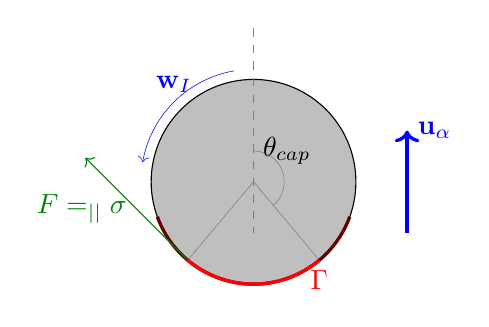
\begin{tikzpicture}[scale =1.3]
        \draw[fill=lightgray](0,0) circle (1);
        \draw[very thin,gray](230:1)--(0,0)--(310:1);
        \draw[very thin,gray](0,0)++(310:0.3) arc (-50:90:0.3)node[right,black]{$\theta_\text{cap}$};
        \draw[very thin,blue,->](0,0)++(100:1.1) arc (100:170:1.1)node[midway,above]{$\textbf{w}_I$};
        \draw[very thick,red!40!black](0,0)++(200:1) arc (200:340:1);
        \draw[very thick,red](0,0)++(230:1) arc (230:310:1)node[below]{$\Gamma$};
        \draw[very thick,blue,->](1.5,-0.5)--++(0,1)node[right]{$\textbf{u}_\alpha$};
        \draw[dashed,gray](0,1.5)--++(0,-2);
        \draw[red,->,green!50!black](230:1)--++(-1,1)node[midway,left]{$F = \nablab_{||} \sigma$};
    \end{tikzpicture}
    \caption{Schematization of the stagnant-cap regime for a
    spherical rising bubble in a quiescent liquid.}
    \label{fig:contaminated_bubbles}
\end{figure}


It can be shown that at the microscale level $C_I$ and $C_k$ follows these conservation laws \citep{pesci2018computational,manikantan2020surfactant}, 
\begin{align*}
    \pddt C_1
    + \nablabh \cdot (\textbf{u}_1 C_1)
    &= D \Delta C_1
    \;\;\; \text{on} \;\;\; \Omega_1\\
    \pddt C_I
    + \nablabhI \cdot (\textbf{u}_I C_I)
    &= D_I \Delta_{||} C_I
    \;\;\; \text{on} \;\;\; \Sigma,
\end{align*}
where $D$ and $D_I$ are the volume and surface diffusion coefficient, respectively. 
The operator $\Delta = \nablabh \cdot (\nablabh\ldots)$ and $\Delta_{||}= \nablabhI \cdot (\nablabhI\ldots)$ are the volume and surface Laplacian operator, respectively.

Now that the microscale equations are well posed we can easily derive the averaged equations for $C_1$ in the continuous phase based on \ref{eq:avg_dt_chi_f}. 
From these considerations the averaged conservation law of $C_1$ the continuous reads, 
\begin{equation}
    \pddt (\phi_1 \oneavg{C_1})
    + \nablab \cdot (\phi_1 \oneavg{C_1} \oneavg{\textbf{u}_1})
    = D \Delta (\phi_1\oneavg{C_1}) 
    - \pnavg{b_\alpha}
    +  \nablab \cdot \textbf{B}
    \label{eq:hybrid_avg_dt_C}
\end{equation}
where $b_\alpha$ is the exchange term with the dispersed phase given by, 
\begin{equation*}
    b_\alpha
    = \int_{\Sigma_\alpha}
    D(\nablabh C_1 ) 
\cdot \textbf{n}_2d\Sigma.
\end{equation*}
The interagrand of $b_\alpha$ is equivalent to the Kinetically controlled sorption boundary condition\citet{pesci2018computational}. 
We recover as in \citet{manikantan2020surfactant} that the term $D(\nablabh C_1) \cdot \textbf{n}_2$ acts as an exchange terms in the surface surfactant concentration equation. 
In \citet{manikantan2020surfactant} it is modeled as a source, denoted $j_n$ in their article.
In fact, it can b shown that Equation (3.9) of \citet{manikantan2020surfactant} correspond to \ref{eq:dt_delta_I_f_I} with $f_I = \Gamma$. 
\tb{disscus the possible closure found by \citet{kentheswaran2022direct}}
Nevertheless, due to the dispersed phase averaging process an additional term arise in the transport of the concentration $C_1$. 
Indeed, the dissipative term $B_\alpha$ can be expressed by, 
\begin{equation*}
    B_\alpha
    =     
    \frac{s_\alpha n_p}{a}\pnnavg{C_\alpha\textbf{r}_c}
    + \oneavg{C'_1\textbf{u}_1'}
    - aD\pnavg{\int_{\Sigma_\alpha} \textbf{n}_2
    (\nablabh C_1)
\cdot \textbf{n}_2d\Sigma}
\end{equation*}
The last term represent the first moment of the Kinetically controlled sorption boundary condition, together with the integrated value of $C_1$ on the surface of the particle. 


For the dispersed phase we first wish to solve an equation for the mean surface surfactant concentration $C_\alpha$. 
From \ref{eq:avg_dt_dq_alpha_tot} the averaged linear conservation equation of $C_\alpha$ reads as, 
\begin{equation}
    \pddt (\pnavg{C_\alpha})
    + \nablabh \cdot (\pnavg{\textbf{u}_\alpha} \pnnavg{C_\alpha} + \pnavg{\textbf{u}_\alpha' C'_\alpha})
    = 
    \frac{\pnavg{b_\alpha}}{s_\alpha}
    \label{eq:avg_dt_dC_alpha_tot}
\end{equation}
The fluctuation terms in \ref{eq:avg_dt_dC_alpha_tot} has great chances to be non-negligible as the rising velocity of a bubble is greatly correlated with $C_\alpha$. 
Additionally, one can notice that the diffusive term $D_I \nablabhI \Gamma$ plays no role in the resultant of surfactant. 

By making use of \ref{eq:avg_dt_dG_alpha_tot} together with \ref{eq:avg_dt_dQ_alpha_tot} we can also derive an equation for the mean position of the surfactant, $\textbf{r}_c$, along the surface. 
It has the form :
\begin{multline}
    \pddt (\pnavg{\textbf{r}_\Gamma})
    + \nablabh \cdot (\pnavg{\textbf{u}_\alpha\textbf{r}_\Gamma})
    =
    - \frac{n_p}{s_\alpha}\pnnavg{\frac{\textbf{r}_c}{C_\alpha}b_\alpha}
    + \frac{n_p}{s_\alpha}\pnnavg{
        \frac{1}{C_\alpha}
        \int_{\Sigma_\alpha} \left[
        \Gamma \textbf{w}_I
        - D_I (\nablabhI \Gamma)
    \right] d\Sigma}\\
    + \frac{n_p}{s_\alpha}\pnnavg{
    \frac{1}{C_\alpha}
    \int_{\Sigma_\alpha} \textbf{r} \left[
        D(\nablabh C_1)
    \right]\cdot \textbf{n}_2  d\Sigma}.
    \label{eq:avg_dt_dG_alpha_tot}
\end{multline}
Let examine each source terms. 
The first term on the RHS represent the change in center of surfactant due to the isotropic exchange with the bulk phase. 
The other exchange term account for the anisotropic apport of surfactant over the surface of the particle.
This term might be of great importance since the bubble's surface will absorbed more surfactant in low concentrated zone.  
The second term account for the surfactants diffusion and advection over the droplet surface. 
The latter being probably neglectable as in \citet{kentheswaran2022direct}. 
In the high area density 
In a steady state regime it be shown that $C_I \textbf{w}_I = 0$ also 



This vector directly gives a relation on the $\theta_\text{cap}$ which is correlated by the drag. 
According to the scheme
\begin{align*}
    |\textbf{r}_c| s_\alpha
    &=a^2 C_I \int_{0}^{2\pi} \int_{0}^{\theta_\text{cap}}  \sin\theta \textbf{r}_z d\phi d\theta\\
    &=a^2 C_I \int_{0}^{2\pi} \int_{0}^{\theta_\text{cap}}  \sin\theta a \cos\theta d\phi d\theta\\
    &=a^3 C_I \pi \cos^2{\theta_\text{cap}}
\end{align*}
so $r_z = \frac{1}{2}a C_I \cos^2{\theta_\text{cap}}$
Due to the complexity of the problem we won't develop further in this work. 
The main takeaway here is to understand that these first and higher order moment equation are tools to describe the dispersed phase at any order of accuracy regardless of the problem treated. 

\tb{Add "surfactant dynamic" }
\tb{with the exchange with the bulk}
\tb{Open on surfactant bubbbly flow with the JFM review and bothe}
\tb{Open non fore-after axissymmetric particle}


\tb{Extends to solid mechanics with deformable particle and composite}

\tb{
\subsubsection*{Oblate bubbles}

As it has already mentioned the trace of the moment of momentum equation can be used to derive the Reyl
It is also possible to derive from the second moment of mass equation an equation for the mean aspect ratio $\pnnavg{\xi}$ of the particles. 
Indeed, let's consider obalte particles, such as droplets or bubble, in this case the second moment of mass can be written, $\mathcal{M}_\alpha =  \textbf{pp} [M_\alpha^{||}(t) - M_\alpha^\bot(t)] +  \textbf{I} M_\alpha^\bot(t)$
\tb{As in tomiyama example they state that the shape of the particle is of particular importance here the moment of volume matter }


\subsubsection*{Spherical compressible bubbles}
As mentioned in the \ref{sec:Lagrangian} from teh trace of the moment of momentum equation we can recover the Rayleigh-Lamb-Plesset equation. 
Thus, by using the averaged moment of momentum equation we can falll back on \citet{zhang1994ensemble} model. 

\subsubsection*{Slightly deformable elastic particle}

Now let consider the momentum conservation of slightly deformable particles. 
First, the velocity field inside the particles, is assumed linear and incompressible, such that $\textbf{u}(\textbf{y}_\alpha) = \textbf{u}_\alpha + \mathcal{L}_\alpha \cdot \textbf{r}$ where the second order tensor  $\mathcal{L}_\alpha= \textbf{e}_\alpha+ \boldsymbol{\omega}$, with $\textbf{e}$ and $\boldsymbol{\omega}$ are symmetric and skew-symmetric tensors, respectively.
It directly follows from the expression of the velocity : $\mathcal{P}_\alpha = \int_{\Omega_\alpha} \textbf{r}\textbf{u} d\Omega = \mathcal{L}_\alpha\cdot \mathcal{M}$
 
The constitutive equation of the stress, $\textbf{T}_2$, within the particle phase can be written such as $\textbf{T}_2 = \mathbb{C} : \textbf{e}_2$ for elastic materials, with $\mathbb{C}$ the fourth order stiffness tensor and $ \textbf{e}_2 = \frac{1}{2}\left(\nablab\textbf{u}_2+(\nablab\textbf{u}_2)^T\right)$ is the rate of strain symmetric tensor. 
Making use of the internal velocity expression yield directly the relation, $\textbf{e}_2=\textbf{e}_\alpha\cdot$ in $\Omega_\alpha$. 

We know that the deformation of the particles will not have an explicit impact on the linear conservation equations.
Thus, we will be interested into the first and second order momentum and mass conservation equations respectively.   
Making use of the average of \ref{eq:dt_P_alpha} over every configuration of the flow, and using the previous properties yield an equation for the average stress tensor within the suspension, namely, 
\begin{equation}
    \pnnavg{\int_{\Omega_\alpha}\textbf{T}_\alpha d\Omega}
    = n_p\mathbb{C} : \pnnavg{(\mathcal{L}_\alpha+ \mathcal{L}_\alpha^T) v_\alpha}
    % = - \mathcal{L}_\alpha\cdot \mathcal{L}_\alpha\cdot \mathcal{M}_\alpha
    % - \mathcal{M}_\alpha \cdot\ddt \mathcal{L}_\alpha
    % - \textbf{M}_\alpha
    \label{eq:hybrid_avg_dt_P_alpha}
\end{equation}
\begin{equation}
    \mathcal{M}_\alpha \cdot\ddt \mathcal{L}_\alpha
    = - \mathcal{L}_\alpha\cdot \mathcal{L}_\alpha\cdot \mathcal{M}_\alpha
    - \mathbb{C} : (\mathcal{L}_\alpha+ \mathcal{L}_\alpha^T) v_\alpha
    - \textbf{M}_\alpha
    \label{eq:hybrid_avg_dt_P_alpha}
\end{equation}
Besed on that kind of argument \citet{lhuillier1987phenomenology}
}



\section{Discussion and conclusion}
\section{Conclusion}
\label{sec:conclusion}




In this work, we aimed to present a complete exposition of the averaged equations and the derivation of closures for complex dispersed phases. 
The general derivation carried from \ref{sec:local_eq} to \ref{sec:equivalence} explains in detail the structure of the system of averaged equations under the so-called hybrid formulation.  
To illustrate our approach, in \ref{sec:closure}and \ref{sec:averaged_surface} we study the example of a dilute viscous-dominated suspension of droplets, including non-uniform surface tension effects. 
We demonstrated how surface tension gradients induce a momentum source, which is responsible for the Marangoni drift of the dispersed phase, and how they also lead to non-Newtonian behavior in the momentum equations. 
Then, we determined how to calculate the averaged shape of the droplets based on the moment of momentum equations. 
An obvious perspective of this work is to use the surfaces Lagrangian-averaged equations to properly derive the transport equations for surfactant concentration (or temperature field), thereby relating surface tension gradients to physical quantities.  


On another note, there have been very few efforts to extend these results to finite Reynolds number regimes, despite the fact that most flows of interest exhibit inertial characteristics. 
\citet{stone2001inertial} demonstrated that, in the case of general linear flow, the effect of finite inertia is to produce normal stresses, leading to non-Newtonian behavior, while the effective viscosity remains unchanged with respect to Einstein's original formula. 
This prediction was extended to the case of drops by \citet{raja2010inertial}. 
However, in these works they only consider neutrally buoyant particles, hence neglecting the effects of relative motion on the suspension rheology. 
To provide a first glimpse of how inertial effects could impact the suspension rheology and droplet deformation, we need to find at least the first order correction in $\mathcal{O}(Re)$ of the closure terms in \ref{eq:dt_hybrid_Sp} and \ref{eq:dt_uf2}. 
Based on symmetry arguments (similar to those used for \ref{eq:Reynolds_stress_functional_form}) one may state that the stresslet is given by, 
\begin{equation}
    \pSavg{\textbf{r}\bm\sigma^*_f\cdot \textbf{n}}
    -\pOavg{2\mu_f\textbf{e}^*_f}
    =
    Re \phi 
    \left[
       C_s^1 \textbf{u}_{r}\textbf{u}_{r} 
    +  C_s^2 (\textbf{u}_{r}\cdot \textbf{u}_{r})\bm\delta
    \right]
    + O(Re^2,\phi^2),
    \\
\end{equation}
at the first order in Reynolds number. 
We conclude that at finite Reynolds number relative motions impact the shape balance of the particle, at least through this term (in agreement with \citet{taylor1964deformation}) and the counterpart is that it induces stresses in the suspension proportional to $\sim \textbf{u}_r\textbf{u}_r$ in addition to the contribution of the Reynolds stress \eqref{eq:Reynolds_stress_functional_form}. 
In a work in preparation we investigate the effects of drop translation at finite Reynolds numbers on the stresslet, notably we provide the exact values of the constant $C_s^{1}$ and $C_s^{2}$ (see also \citet{fintzi2025}). 
 


%\end{enumerate}
%=======
%\item \tb{
%    Note that in the continuous phase conservation equation \eqref{eq:avg_hybrid_dt_chi_f}, in the total volume conservation \ref{eq:volume_conservation}, and in the bulk velocity formulation \ref{eq:velocity_conservation}, an infinite number of moments are involved. 
%    Hence, the last reason why one may need to obtain such higher moments is because it is required directly by \ref{eq:avg_hybrid_dt_chi_f}, \ref{eq:volume_conservation} and \ref{eq:velocity_conservation}. 
%    As discussed above the moments of hydrodynamic momentum exchanges are crucial to describe the suspension rheology \eqref{eq:avg_hybrid_dt_chi_f}, but also note how the second moment of volume and momentum in \ref{eq:volume_conservation} and \ref{eq:velocity_conservation} are relevant for the stability and hyperbolicity of the system of equations \citep{prosperetti1995finite}. 
%}
%\end{enumerate}
%>>>>>>> 4731d90 (JLP: hybrid)
%Thus, we can conclude that the higher moments $\textbf{Q}_p^{(n)}$ is needed uniquely if the closure terms are highly dependent on this moment, or if the information given by $\textbf{Q}_p^{(n)}$ is the final objective of the study. 
%In conclusion, the higher-order moments, $\textbf{Q}_p^{(n)}$, are specifically required if the closure terms are significantly influenced by this moment or if the primary goal of the study is to analyze the information provided by $\textbf{Q}_p^{(n)}$, \tb{or when they appear explicitly in the conservation law and turns out being non-negligible}.
 %for the unknowns $f_f$,  $Q_\alpha$, $\textbf{Q}_p^{(1)}$\ldots$\textbf{Q}_p^{(n)}$. 

 
 %A priori cela ne vient que du moment d'ordre 2. Le cpt non-newtonien vient de la differente de vitesse

\section*{Acknowledgement}
We would like to express our sincere gratitude to Professor D. Lhuillier for his inspiring and insightful class, which has greatly influenced our work.
Also, the authors are grateful for many in-depth discussions with Professor St\'ephane Popinet from \textit{Institut Jean le Rond Alembert} as well. 
\bibliography{Bib/bib_bulles.bib}



\appendix

\section{Proof of the generalized form of the interfacial balance law}
\label{ap:interface_proof}
% In \citet[Appendix 2]{marle1982macroscopic} they demonstrated how to obtain \ref{eq:dt_delta_I_f_I} in the specific context of the mass, momentum and energy equations. 
For completeness and ease of understanding we give in this appendix the detailed derivation of \ref{eq:dt_delta_I_f_I}. 
Let us first introduce some important relations regarding surface properties. 
Consider the arbitrary tensor $ \textbf{F}_{I}$ defined on $\Gamma(t)$.
Let us take the surface divergence of $\textbf{F}_{I||} = \textbf{F}_I \cdot (\bm\delta -\textbf{nn})$, it yields,
\begin{align}
    \delta_I \divI \textbf{F}_{I||}
    &= 
    \div (\delta_I \textbf{F}_{I||})
    - \textbf{n}(\textbf{n}\cdot\grad)\cdot (\delta_I \textbf{F}_{I||})
    - \textbf{F}_{I}\cdot\gradI\delta_I \nonumber\\
    &= 
    \div (\delta_I \textbf{F}_{I||})
    - \textbf{n}(\textbf{n}\cdot\grad)\cdot (\delta_I \textbf{F}_{I||})
    - \textbf{F}_{I} \delta_I (\textbf{n}\cdot\grad)\textbf{n}
    % &= 
    % \div (\delta_I \textbf{F}_{I||})
    \label{eq:step1}
\end{align}
were we used the chain rule and the relation $\divI(\ldots) = \div(\ldots) - \textbf{n}(\textbf{n}\cdot \grad)\cdot(\ldots)$ for the first equality. 
The second equality is derived using \ref{eq:grad_delta_I} dotted with $(\bm\delta -\textbf{nn})$, which gives the relation 
\begin{equation*}
    (\bm\delta - \textbf{nn}) \cdot \grad\delta_I
    = \gradI \delta_I
    = 
    \delta_I (\textbf{n}\cdot \grad)\textbf{n}.
\end{equation*}
Expanding the second term of \ref{eq:step1} by noticing that $\textbf{F}_{I||} = (\bm\delta - \textbf{nn})\cdot \textbf{F}_I$, and using the expression $\textbf{n}(\textbf{n}\cdot\grad)\cdot (\bm\delta - \textbf{nn}) =  (\textbf{n}\cdot\grad)\textbf{n}$
% \begin{equation*}
%     - \textbf{n}(\textbf{n}\cdot\grad)\cdot (\delta_I \textbf{F}_{I||})
%     = 
%     - \delta_I \textbf{F}_{I}\textbf{n}(\textbf{n}\cdot\grad)\cdot (\bm\delta - \textbf{nn})
%     + (\bm\delta - \textbf{nn}) \cdot \textbf{n}(\textbf{n}\cdot\grad)(\delta_I \textbf{F}_{I})
%     = \textbf{F}_{I} \delta_I (\textbf{n}\cdot\grad)\textbf{n},
% \end{equation*}
 leads us to the useful relation :
\begin{equation}
    \delta_I \divI \textbf{F}_{I||}
    = 
    \div (\delta_I \textbf{F}_{I||}). 
    \label{eq:proof_1}
\end{equation}
% Making use of the same principles one can show the already common expression  
% \begin{equation}
%     \divI
%     \textbf{F}_{I}
%     = 
%     \divI
%     \textbf{F}_{I||}
%     +(\textbf{F}_I \cdot \textbf{n})  \div \textbf{n},
% \end{equation}
% which, multiplied with $\delta_I$ gives 
% \begin{equation}
%     \delta_I \divI
%     \textbf{F}_{I}
%     = 
%     \div
%     (\delta_I \textbf{F}_{I||})
%     +\delta_I (\textbf{F}_I \cdot \textbf{n})  \div \textbf{n}. 
%     \label{eq:proof_1}
% \end{equation}


To demonstrate that \ref{eq:dt_delta_I} and \ref{eq:dt_delta_I_f_I} are consistent we must prove the equality 
\begin{equation}
    \delta_I
    \left[ \pddt f_I^0 
    + f_I^0 (\textbf{u}_{I}^0\cdot \textbf{n})  (\div \textbf{n})
    +\divI
    (f_I^0 \textbf{u}_{I||}^0
    - \mathbf{\Phi}_{I||}^0 )
    \right]
    =
    \pddt (\delta_If_I^0) 
    +\div
    (\delta_If_I^0 \textbf{u}_I^0
        - \delta_I\mathbf{\Phi}_{I||}^0 ).
    \label{eq:to_prove}
\end{equation}
This is easily done  using \ref{eq:dt_f_I} on the two first terms on the left-hand side of \ref{eq:to_prove} which gives
\begin{equation*}
    \delta_I \pddt f_I^0 
    + f_I^0 \delta_I (\textbf{u}_I\cdot\textbf{n})(\div \textbf{n})
    = 
     \pddt (f_I^0 \delta_I)
    + \div(f_I^0  \delta_I \textbf{n}(\textbf{n}\cdot\textbf{u}_I^0)). 
    % - \delta_I (\textbf{n}\cdot\textbf{u}_I^0) (\textbf{n}\cdot \grad)f_I^0. 
\end{equation*}
Where it is assumed that $\delta_I (\textbf{n}\cdot\textbf{u}_I^0)(\textbf{n}\cdot\grad) f_I^0 = 0$ for reasons discussed in detailed in \citet{orlando2023evolution,estrada1985distributional}. 
Then, using the relation \ref{eq:proof_1} on the remaining terms on the left-hand side of \ref{eq:to_prove} directly proves \ref{eq:to_prove} and by extension \ref{eq:dt_delta_I_f_I}. 





\section{Arbitrary order moments equation}
\label{ap:Moments_equations}

Let's define the arbitrary moment of the tensor $f$, by, 
\begin{equation*}
    Q_{i_1\ldots i_n}
    = \int_{V_\alpha} 
    \pri{1}{n} f dV
\end{equation*}
Then,
\begin{multline*}
    \ddt Q_{i_1\ldots i_n}
    =\int_{V_\alpha} \left[ \partial_t \left(\pri{1}{n}f\right) 
    + \partial_k \left(u_k \pri{1}{n}f\right) \right]dV\\
    +\int_{S_\alpha} \pri{1}{n} f \left(u^I_k - u_k\right) n_k dS.
\end{multline*}
Using the product rule on the derivatives yields, 
\begin{multline*}
    \ddt Q_{i_1\ldots i_n}
    =\int_{V_\alpha} f \left[ \partial_t \left(\pri{1}{n}\right) 
    + u_k \partial_k \left( \pri{1}{n}\right) \right]dV\\
    +\int_{V_\alpha} \pri{1}{n} \left[ \partial_t \left(f\right) 
    +  \partial_k \left(u_k f \right) \right]dV\\
    +\int_{S_\alpha} \pri{1}{n} f \left(u^I_k - u_k\right) n_k dS.
\end{multline*}
From similar arguments as before one can easily show that, 
\begin{multline*}
    \ddt Q_{i_1\ldots i_n}
    = \sum_{e=1}^{n} \int_{V_\alpha} f  \prod^{n}_{\substack{ m=1 \\   m \neq e}} r_{i_m} w_{i_e}dV
    +\int_{V_\alpha} \pri{1}{n} \nablabh\cdot\mathbf{\Phi} dV\\
    + \int_{V_\alpha} \pri{1}{n} \textbf{S} dV
    +\int_{S_\alpha} \pri{1}{n} f \left(u^I_k - u_k\right) n_k dS.
\end{multline*}
The second term can be reformulated such as,
\begin{align*}
    \int_{V_\alpha} \pri{1}{n} \nablabh\cdot\mathbf{\Phi} dV
    &= \int_{S_\alpha} \nablabh \cdot \left(\pri{1}{n} \mathbf{\Phi} \right)dV
    - \int_{V_\alpha} \mathbf{\Phi} \cdot \nablabh \left(\pri{1}{n} \right)dV\\
    &= \int_{S_\alpha} \pri{1}{n} \mathbf{\Phi} \cdot \textbf{n}dS
    -\sum_{e=1}^{n} \int_{V_\alpha} \mathbf{\Phi}  \prod^{n}_{\substack{ m=1 \\m \neq e}} r_{i_m}  dV
\end{align*}
Including this relation into the former equation yields, 
\begin{multline*}
    \ddt Q_{i_1\ldots i_n}
    = \sum_{e=1}^{n} \int_{V_\alpha} \prod^{n}_{\substack{ m=1 \\   m \neq e}} r_{i_m} (w_{i_e}f  - \Phi)dV
    +\int_{S_\alpha} \pri{1}{n} \mathbf{\Phi} \cdot \textbf{n}dS\\
    + \int_{V_\alpha} \pri{1}{n} \textbf{S} dV
    +\int_{S_\alpha} \pri{1}{n} f \left(u^I_k - u_k\right) n_k dS.
\end{multline*}
Then it is possible from this equation to carry out a particular average but also to get the local scale equations. 
Indeed, if we consider $V_\alpha$ as being a fixed control volume the above equality can be rewritten such as, 
\begin{multline}
    \pddt \left(\pri{1}{n}f\right)
    + \nablabh \cdot \left(\pri{1}{n}f \textbf{u}\right)
    = n  \pri{1}{n-1}  (w_{i_n}f  - \Phi)\\
    + \pri{1}{n} \textbf{S} 
    + \nablabh \cdot \left( \pri{1}{n} \mathbf{\Phi} \right)
    \label{ap:eq:dt_Q_alpha_n}
\end{multline}


% In this section we propose to study two example. 
This objective is to demonstrate how to derive specific application from our general hybrid model. 
Secondly, we wish to point out in wish situation one needs or might not need the more than the zeroth order equation of the particle phase.

% \subsection{Solid axis symmetric particle suspension}

% Let's start by the second moment of mass averaged equation.
As a first example let examine the case of a mono-disperse axissymmetric suspension of solid particles, such as ellipsoid or cylinders.
Let the vector $\textbf{p}$ denote the unit vector representing the orientation of the particle along its main axis of inertia. 
Then, the second moment of mass can be written as $\mathcal{M}_{\alpha,ij} =  p_ip_j M_\alpha^{||} +  \delta_{ij} M_\alpha^\bot$, where $M_{\bot}$ and $M_{||}$ represent the coefficients corresponding to the principal directions of the particles' mass distribution.
It is well-established that at least the drag force exhibits a significant dependence on the orientation of the particle \citep{kim2013microhydrodynamics}.
Therefore, despite being a second-order moment, the particle field $\mathcal{M}_p$ is indispensable to close the mono-disperse axissymmetric suspension problem.
We will see that to determine the orientation of the particles one need to know about its angular velocity, which give the use to the equation for $\mathcal{P}_p$, equally.  


% \subsubsection{Single particle equations}

We first focus on the one particle dynamic before deriving the averaged equations. 
As stated above we assume the velocity of the dispersed phase to be of the form : $u_{2,i}^0(\textbf{x}_\alpha + \textbf{r}) = u_{i}^\alpha + \epsilon_{ijk} {\omega}_{j}^\alpha {r}_k$, with $\omega_{a}^\alpha$ the angular velocity of the particle $\alpha$ and $\epsilon$ the Levi-Cita symbol.
Injecting this definition of the velocity in \ref{eq:mu_def}, \ref{eq:S_def} and \ref{eq:E_def} one can re-write the moment of momentum skew-symmetric and symmetric part and the internal energy equation, of the particle as,
\begin{align}
    % \label{eq:S_def}
    2\mathcal{S}_{\alpha,ij}
    % = \Omega_{\alpha,jk} \mathcal{I}_{\alpha,ki} + \Omega_{\alpha,ik} \mathcal{I}_{\alpha,kj}
    = - \epsilon_{jak} \omega_a^\alpha \mathcal{I}_{ki}^\alpha
      - \epsilon_{ibk} \omega_b^\alpha \mathcal{I}_{kj}^\alpha
    % = 
    % M_\alpha^{||}  \left(
    %     \epsilon_{ikl} \omega_k 
    %     p_lp_j 
    %     +  \epsilon_{jkl} \omega_k 
    %     p_lp_i 
    % \right)
    \\
    % \label{eq:mu_def}
    \mu_{\alpha,i}
    % = 
    % \omega_{\alpha,j}(\mathcal{M}_{\alpha,kk} \delta_{\alpha,ij} - \mathcal{M}_{\alpha,ij})=
    % \omega_j \left[
    %     \delta_{ji} (M_\alpha^{||} + 2M_\alpha^\bot)
    %     - p_jp_i M_\alpha^{||} 
    % \right]
    =  \mathcal{I}_{ij}^\alpha \omega^\alpha_j\\
    2W_\alpha 
    = \omega^\alpha_k\omega^\alpha_l \mathcal{I}_{kl}^\alpha
\end{align}
Under this form notice that the angular momentum is the product of the angular velocity $\omega_{\alpha,i}$ times $\mathcal{I}_{ik}^\alpha = (\mathcal{M}_{kk}^\alpha \delta_{ij} - \mathcal{M}_{ij}^\alpha)$ which is consistent with the definition of the moment of inertia used in solid mechanics.
In fact, it has been found  more practical to express the following equation with $\mathcal{I}_\alpha$ rather than with $\mathcal{M}_\alpha$. 
Thus, in this section we express all closure and equation with respect to $\mathcal{I}_\alpha$
Now we make use of the preceding definition to rewrite the first moment of mass, angular momentum and internal energy equation, i.e. \ref{eq:dt_M_alpha}, \ref{eq:dt_P_alpha} and \ref{eq:dt_w2_alpha}, gives directly, 
\begin{align}
    \label{eq:dt_I_alpha}
    \ddt \mathcal{I}_{ij}
    = - \epsilon_{jak} \omega_a^\alpha \mathcal{I}_{ki}^\alpha + 
    - \epsilon_{ibk}   \omega_b^\alpha \mathcal{I}_{kj}^\alpha\\
    \label{eq:dt_Iomega_alpha}
    \ddt (\mathcal{I}_{ij}^\alpha \omega_j^\alpha)
    = t^\alpha_i\\
    \label{eq:dt_Iomegaomega_alpha}
    \frac{1}{2}\ddt (\omega^\alpha_k\omega^\alpha_l \mathcal{I}_{kl}^\alpha)
    = \omega_k t^\alpha_k. 
\end{align}
As, can be seen here the dependence of the inertia matrices with time induce a significant complication to the problem. 
Firstly we must keep track of the evolution of the inertia matrices which add one supplementary equation. 
Secondly, the angular momentum and angular kinetic energy of the particle is not function solely of the angular velocity but also on its own inertia matrices. 
Which will add difficulty to unpair to angular velocity from the inertia matrix in the averaged equation. 

% \tb{maybe add the heat issipation}
% It will be useful in the following derivation to have an equation for $\omega_i^\alpha$, manipulating the equation of angular momentum with the use of the equation of evolution of the inertia matrix we obtain, 
% \begin{equation}
%     \ddt (\omega_i^\alpha)
%     = (\mathcal{I}^\alpha)_{ik}^{-1}(  
%         t^\alpha_k
%     -  \mathcal{S}_{kl}^\alpha\omega_l^\alpha
%     )
% \end{equation}
% Taking the dot product of this equation with $\omega_j^\alpha$ and adding its transpose in the indices $ij$ gives, 
% \begin{equation}
%     \ddt (\omega_i^\alpha\omega_j^\alpha)
%     = 
%     \omega_j^\alpha
%     (\mathcal{I}^\alpha)_{ik}^{-1}(  
%         t^\alpha_k
%     -  \mathcal{S}_{kl}^\alpha\omega_l^\alpha
%     )
%     + \omega_i^\alpha
%     (\mathcal{I}^\alpha)_{jk}^{-1}(  
%         t^\alpha_k
%     -  \mathcal{S}_{kl}^\alpha\omega_l^\alpha
%     )
% \end{equation}

% Also, notice that the stress within the particle is supposed to be unknown. 
% Indeed, we considered rigid body motion inside the particles.
% However, it is still possible to evaluate the stress using the stretch of momentum equation which in this case yields, 
% \begin{equation*}
%     \intO{(\sigma_2^0)_{ij}}
%     = 
%     - \ddt \mathcal{S}^\alpha_{ij}
%     + \epsilon_{iab}\epsilon_{ibd}\omega_{b}^\alpha\omega_{d}^\alpha(
%         \frac{1}{2}\mathcal{I}_{kk}\delta_{ac}
%         - \mathcal{I}^\alpha_{ac} )
%     + S^\alpha_{ij}.
%     \\
% \end{equation*}
% Therefore, the stress can be computed conditionally on the knowledge of the angular velocity and acceleration of the particle, which can be determinate by solving the previous equations. 
% It is then possible to validate the hypothesis of deformable particle  upon the knowledge of the material body law. 

% Finally, in the perspective of deriving an equation for the covariance of the translational motion and the orientation we multiply the equation of $\mathcal{I}_{ij}^\alpha$ by $u_k^\alpha$ and the equation of $u_k^\alpha$ by $\mathcal{I}_{ij}^\alpha$, which gives us get the following equation,
% \begin{equation*}
%     \ddt (\mathcal{I}_{ij}^\alpha u_k^\alpha)
%     =
%     u_k^\alpha
%     \ddt \mathcal{I}_{ij}^\alpha
%     + \mathcal{I}_{ij}^\alpha \ddt u_k^\alpha
%     = u_k^\alpha \mathcal{S}_{ij}^\alpha
%     +  \mathcal{I}_{ij}^\alpha g_k
%     +  \mathcal{I}_{ij}^\alpha f_k^\alpha/m^\alpha
% \end{equation*}

% \subsubsection{Averaged equation for the fluid phase}

% It is somewhat simpler to first modify the fluid phase equations. 
% Indeed, among the 4 equations to be solved only the terms involving the internal velocity will be explicitly modified.  
% These terms appear in \ref{eq:dt_hybrid_k1}, under the form $\pSavg{{\textbf{rw}_2^0\times\bm{\sigma}_1^0 \cdot \textbf{n}_2}}$, where we substitute $\textbf{w}$ for the expression of a solid particle velocity field. 
% Substituting these terms into the pseudo turbulent energy equation gives, 
% \begin{multline*}
%     \pddt (\phi_1\rho_1k_1)  
%     + \div (
%         \phi_1\rho_1k_1\textbf{u}_1
%         + \textbf{q}_1^\text{k} 
%         )
%     = 
%     - \avg{\chi_1\bm{\sigma}_1^0 : \grad \textbf{u}_1^0}
%     - \bm{\sigma}_1^\text{eq} : \grad \textbf{u}_1
%     + (\textbf{u}_1 - \textbf{u}_p)
%     \cdot \pSavg{{\bm{\sigma}_1^0 \cdot \textbf{n}_2}}\\
%     - \pavg{ \textbf{u}^{\alpha'} \cdot \intS{  \bm{\sigma}_1^0 \cdot \textbf{n}_2}}
%     - \bm{\omega}_{p} \cdot  \pavg{\intS{\textbf{r}\times\bm{\sigma}_1^0 \cdot \textbf{n}_2}}
%     - \pavg{\bm{\omega}^{'}_\alpha  \cdot \intS{\textbf{r} \times \bm{\sigma}_1^0 \cdot \textbf{n}_2}}
%     % \pSavg{\textbf{r}\textbf{w}^0_2 \cdot \textbf{r}\bm{\sigma}_1^0 \cdot \textbf{n}_2}_l
% \end{multline*}
% with,
% \begin{multline*}
%     \textbf{q}_1^\text{k}
%     = \rho_1 \avg{\chi_1 \textbf{u}_1' k_1} 
%     - \avg{\chi_1 \textbf{u}_1' \cdot \bm{\sigma}_1^0}
%     + (\textbf{u}_1 - \textbf{u}_p)\cdot
%     \pSavg{{\textbf{r}\bm{\sigma}_1^0 \cdot \textbf{n}_2}}
%     \\
%     - \pavg{ \textbf{u}_\alpha' \cdot \intS{ \textbf{r} \bm{\sigma}_1^0 \cdot \textbf{n}_2}}
%     - \epsilon_{ijk} \omega_{p,j} \pavg{ \intS{\textbf{rr}\bm{\sigma}_1^0 \cdot \textbf{n}_2}}_{kli}
%     - \epsilon_{ijk}\pavg{\omega^{\alpha'}_{j}  \intS{\textbf{rr}\bm{\sigma}_1^0 \cdot \textbf{n}_2}}_{kli}
% \end{multline*}
% Now, we clearly see appear the mean and fluctuating work due to the rotational motion of the particles. 
% Which are the product of the angular velocities times the torque on the surface of the particles. 
% Similar comments can be made for the flux term were we see appear the work of the second moments of the surface traction with the angular velocity. 

% By the assumption of solid particle motion we already reformulated the closure terms of the form $\pSavg{{\textbf{rw}_2^0\times\bm{\sigma}_1^0 \cdot \textbf{n}_2}}$ surface traction tensor which were already present in the problem. 
% Nevertheless, we still now need to find additional closure related to the angular velocity covariance with the torque. 

% \begin{align*}
%     \pSavg{\textbf{w}^0_2\cdot \bm{\sigma}_1^0 \cdot \textbf{n}_2}
%     =
%     \epsilon_{ijk}\omega_{p,j}  \pavg{\intS{\textbf{r}\bm{\sigma}_1^0 \cdot \textbf{n}_2}_{ki}}
%     + \epsilon_{ijk}\pavg{{\omega}^{\alpha'}_{j}  \intS{\textbf{r}\bm{\sigma}_1^0 \cdot \textbf{n}_2}_{ki}}\\
%     \pSavg{\textbf{r}\textbf{w}^0_2 \cdot \textbf{r}\bm{\sigma}_1^0 \cdot \textbf{n}_2}_l
%     =
%     \epsilon_{ijk} \omega_{p,j} \pavg{ \intS{\textbf{rr}\bm{\sigma}_1^0 \cdot \textbf{n}_2}_{kli}}
%     + \epsilon_{ijk}\pavg{\omega^{\alpha'}_{j}  \intS{\textbf{rr}\bm{\sigma}_1^0 \cdot \textbf{n}_2}_{kli}}
% \end{align*}


\subsubsection{Orientation equation in stoke regime.}

Averaging the second-order moment of mass yields, $n_p \mathcal{M}_p =  \textbf{A}_p (M_p^{||} - M_p^\bot) +  \textbf{I} M_p^\bot$ where $\textbf{A}_p$ is the orientation tensor defined as $\textbf{A}_p = \avg{\delta_\alpha\textbf{pp}}$.
Then, let's express the internal motion of a solid particle by : $\textbf{u}_2(\textbf{x}_\alpha) = \textbf{u}_\alpha + \textbf{r}\times \omega_\alpha$ where $\omega_\alpha$ represents the angular velocity of the particle.
It follows the expression of the stretching of momentum : $\mathcal{S}_\alpha = (M_\alpha^{||} - M_\alpha^\bot) \left(
    \omega_\alpha \times
    \textbf{pp}
    + \textbf{pp} \times \omega_\alpha
\right)$. 
Subsequently,  we can easily derive the transport equation for $\textbf{A}$ by averaging \ref{eq:dt_M_alpha} and using the previous expressions for $\mathcal{M}_\alpha$ and $\mathcal{S}_\alpha$.
The resulting equation is given by~:
\begin{equation}
    \pddt (n_p\textbf{A})
    + \div (
        n_p\textbf{u}_p\textbf{A}_p
        + \mathbf{\Sigma}
        )
    =
    \pavg{\textbf{pp} \times \omega_\alpha}
    + \pavg{\omega_\alpha \times \textbf{pp}},
    % + \pnavg{\textbf{pp}' \times \omega_\alpha'}
    % +\pnavg{\omega_\alpha' \times \textbf{pp}'}
    \label{eq:avg_dt_M_alpha}
\end{equation}
where $\mathbf{\Sigma} = \pavg{\textbf{u}'_\alpha(\textbf{pp})'}$ is the covariance term between the fluctuation of the velocity and the orientation tensor.
We recall that the definition of the fluctuation notation is provided by the expression from \ref{eq:def_fluctu}.
At this stage we need to find closure for both terms on the RHS of \ref{eq:avg_dt_M_alpha}. 
Therefore, we assume torque free rigid particle in to Stokes flow, where we can utilize Jeffery's equation \citep{guazzelli2011}.
It reads,
\begin{equation}
    \omega_\alpha \times \textbf{p}
    = \mathbf{\Omega}\cdot\textbf{p}
    + \beta\left(
        \textbf{E}\cdot \textbf{p}
        - \textbf{E} : \textbf{ppp}
    \right),
    \label{eq:jefferey}
\end{equation}
with $\textbf{E}$ and $\mathbf{\Omega}$ being the symmetric and antisymmetric parts of the bulk velocity gradient, respectively, such that $\grad\avg{\textbf{u}}=\textbf{E}+\mathbf{\Omega}$.
The coefficient $\beta$  is a constant related to the aspect ratio of the particle.
Finally, by substituting the RHS terms of \ref{eq:avg_dt_M_alpha}, by using \ref{eq:jefferey}, we arrive at the closed form of the second moment of mass equation~:
\begin{equation}
    \pddt \textbf{A}
    + \div (
        \pnnavg{\textbf{u}_\alpha}\textbf{A}
    )
    =
    \mathbf{\Omega} \cdot \textbf{A}
    - \textbf{A} \cdot \mathbf{\Omega}
    + \beta\left[
        \textbf{E} \cdot \textbf{A}
        -\textbf{A} \cdot \textbf{E}
        - \textbf{E} : \mathbb{A}
    \right]
    - \div \mathbf{\Sigma}
    \label{eq:hybrid_avg_dt_pp}
\end{equation}
where the fourth-order tensor $\mathbb{A}$, is defined as $\mathbb{A} = \pavg{\textbf{pppp}}$.
In this expression we removed the fluctuation terms, but they must appear and they are surly not negligible. 
In \citet{wang2008objective} they derive \ref{eq:hybrid_avg_dt_pp} by the means of kinetic theory, based on \ref{eq:jefferey} and the fact that $\ddt \textbf{p} = \omega_\alpha \times \textbf{p}$ (Equation (3) of their article).
Their equation is similar to \ref{eq:hybrid_avg_dt_pp} except that their employ a phenomenological closure for the term, $\div \mathbf{\Sigma}$, which account for particles interactions \tb{je pense que c'est ca mais pas sur}.
Anyhow, we showed how it is possible to derive the orientation tensor conservation equation, commonly used in fiber field theory, from the second-order moments of mass's equation. 
However, \ref{eq:jefferey} is valid in low inertial regime only. 
Therefore, it is indispensable to consider a more general framework when working with inertial particles. 

\subsubsection{Averaged equation for the particle phase}

Now let's turn our attention to the particle phase equations in inertial form. 
We first introduce the average of the inertia matrix, angular momentum and internal energy as,
\begin{align}
    \label{eq:Sp_def}
    2(\mathcal{S}_{p})_{ij}
    = - \epsilon_{jak} \omega_{p,a} \mathcal{I}_{p,ki}
    - \epsilon_{ibk}   \omega_{p,b} \mathcal{I}_{p,kj}
    - \epsilon_{jak} k_{p,kia}^{\mathcal{I}\omega} 
    - \epsilon_{ibk} k_{p,kjb}^{\mathcal{I}\omega}
    \\
    \label{eq:mup_def}
    \mu_{p,i}
    = \mathcal{I}_{p,ij} \omega_{p,j}
    + k_{p,ijj}^{\mathcal{I}\omega}
    \\
    \label{eq:Wp_deformations}
    2 W_p 
    = 
    {\omega}_{p,i}{\omega}_{p,j} \mathcal{I}_{p,ij}
    % \omega_{p,i}\mu_{p,i}
    + \mathcal{I}_{p,ij} {k}^{ww}_{p,ij}
    + 2 {\omega}_{p,i} {k}_{p,ijj}^{\mathcal{I}\omega}
    + k^{Iww}_p
\end{align}
where we introduced the following fluctuating quantities, 
\begin{align*}
    n_p(\textbf{k}_p^{\mathcal{I}\omega})_{ijk}
    = 
    \pavg{\mathcal{I}^{\alpha'}_{ij} \omega^{\alpha'}_k}
    && n_p (k_p^{\omega\omega})_{ij}
    = 
    \pavg{\omega^{\alpha'}_i \omega^{\alpha'}_j}
    && n_p{k}_p^{\mathcal{I}\omega\omega}
    = 
    \pavg{\mathcal{I}^{\alpha'}_{ij} \omega^{\alpha'}_i\omega^{\alpha'}_j}
\end{align*}
Due to the covariance terms, the problem which contained only two unknown at the particle scale, i.e. $\mathcal{I}_\alpha$ and $\bm{\omega}_\alpha$, now contains 5 unknown on the macroscopic scale, i.e. $\mathcal{I}_p$, $\bm{\omega}_p$, $\textbf{k}^{\mathcal{I}\omega}_p$,$\textbf{k}^{ww}_p$ and $\textbf{k}_p^{\mathcal{I}\omega\omega}$
We therefore, need to derive five equation to compute properly the angular momentum and internal fluctuating energy of the particle phase. 


Taking the particle average of \ref{eq:dt_I_alpha},\ref{eq:dt_Iomega_alpha} and \ref{eq:dt_Iomegaomega_alpha} yield the particle average equations for the averaged inertia matrix the angular momentum and the internal kinetic energy, 
\begin{align}
    \label{eq:dt_avg_Ip}
    \pddt (n_p\mathcal{I}_{p,ij})
    + \div (n_p\mathcal{I}_{p,ij} u_{p,k}
    + \mathcal{I}^\text{flux}_{p,ijk})
    = n_p \mathcal{S}_{p,ij},\\ 
    \label{eq:dt_avg_mup}
    \pddt (
    %     n_p \mathcal{I}_{p,ij} \omega_{p,j}
    % + n_p k^{\mathcal{I}\omega}_{p,ijj}
    n_p \mu_{p,i}
    )
    + \div (
        n_p \mu_{p,i}u_{p,k}
    %     n_p \mathcal{I}_{p,ij} \omega_{p,j} u_{p,k}
    % + k^{\mathcal{I}\omega}_{p,ijj} u_{p,k}
    +  \omega_{p,j} \mathcal{I}^\text{flux}_{p,ijk}
    + \mu_{p,ik}^\text{flux}
    )
    = n_p t_{p,i},\\
    \pddt (n_p W_p)
    + \div  (
        n_p W_p u_{p,k}
        + \omega_{p,i} \omega_{p,j}
        \mathcal{I}_{p,ij}^\text{flux}/2
        + \omega_{p,i}\mu_{p,ik}^\text{flux}
    + W_{p,k}^\text{flux}
    )
    = 
    n_p \omega_{p,k} t_{p,k}
    +  \pavg{\omega_k^{\alpha'} t^\alpha_k},
\end{align}
respectively. 
Also, within these averaged equations the correlation of the translational velocity and each of these quantities  appear under the form $(\ldots)^\text{flux}$ have the following expression, 
\begin{align*}
    n_p \mathcal{I}_{p,ijk}^\text{flux}
    = n_p k_{p,ijk}^{\mathcal{I}u}
    = 
    \pavg{\mathcal{I}^{\alpha'}_{ij} u_{k}^{\alpha'}}
    &&
    n_p \mu_{p,ik}^\text{flux}
    = 
    \pavg{\mathcal{I}^{\alpha'}_{ij} \omega^{\alpha'}_j u_{k}^{\alpha'}} 
    + \mathcal{I}_{p,ij} \pavg{u_k^{\alpha'}\omega_j^{\alpha'}}\\
    && n_p W_{p,k}^\text{flux}
    = \frac{1}{2}\mathcal{I}_{p,ij}
    \pavg{
        \omega_j^{\alpha'}
        \omega_i^{\alpha'}
        u_k^{\alpha'}
    }
    + \frac{1}{2}\pavg{
        \mathcal{I}_{ij}^{\alpha'}
        \omega_j^{\alpha'}
        \omega_i^{\alpha'}
        u_k^{\alpha'}
    }.
\end{align*}
At this stage all the fluctuating terms $k^{\ldots}$ can be considered as closure term or as terms to be solved thanks to a secondary transport equations in the same spirit as the pseudo turbulent equation for $k_p$.
Upon substituting $\mathcal{I}_p$ with the orientation vector $\textbf{pp}$ the reader can notice that \ref{eq:dt_avg_Ip} reveal being the equation for the orientation tensor $\pavg{\textbf{pp}}$ \citep{wang2008objective} which is widely used in the fiber suspension study. 
In the context of stokesian suspension the term appearing in the RHS of \ref{eq:dt_avg_Ip} is directly closed through the use of Jeffery's equation \citet{guazzelli2011}.
It leads to a closed equation for the orientation tensor in terms of the derivative of the mean flow field. 
In a more general context, to close the inertia tensor equation and compute the total angular momentum, one needs to obtain an equation for $k^{\mathcal{I}\omega}_{p,ijj}$. 
This is done by first taking the dot product of $\bm{\omega}_{p}$ with \ref{eq:dt_avg_Ip} on the index $j$, then subtracting this expression to \ref{eq:dt_avg_mup}.
This gives rise to an equation for the mean angular velocity and mean fluctuating part of the angular momentum, namely, 
\begin{align}
    \label{eq:dt_avg_kIp}
    \pddt (n_p\mathcal{I}_{p,ij}\omega_{p,j})
    + \div (n_p\mathcal{I}_{p,ij}\omega_{p,j} u_{p,k}
    + \omega_{p,j}\mathcal{I}^\text{flux}_{p,ijk})
    &= 
    n_p \mathcal{S}_{p,ij}\omega_{p,j}
    + \mathcal{I}_{p,ijk}^\text{flux}\grad \omega_{p,j}
    + \mathcal{I}_{p,ij}\pavg{\dot{\omega}^\alpha_j}
    \\
    \label{eq:dt_avg_kIp}
    \mathcal{I}_{p,ij}\left[
        \pddt (n_p\omega_{p,j})
        + \div (n_p\omega_{p,j} u_{p,k})
    \right]
    &= 
    \omega_{p,j}\div\mathcal{I}_{p,ijk}^\text{flux} 
    + \mathcal{I}_{p,ij}\pavg{\dot{\omega}^\alpha_j},
    \\
    \pddt (n_p k^{\mathcal{I}\omega}_{p,ijj})
    + \div (k^{\mathcal{I}\omega}_{p,ijj} u_{p,k}
    + \mu_{p,ik}^\text{flux}
    )
    &= 
    - n_p \mathcal{S}_{p,ij}\omega_{p,j}
    - \mathcal{I}_{p,ijk}^\text{flux}\grad \omega_{p,j}
    - \mathcal{I}_{p,ij}\pavg{\dot{\omega}^\alpha_j}
    + n_p t_{p,i},
\end{align}
respectively. 
The third term in the right hands side of this equation and the mean torque term eventually cancel out leaving only with fluctuating quantities. 
% Now let's turn our attention to the energy parts, 
% \begin{align*}
%     \pddt (n_p\mathcal{I}_{p,ij}\omega_{p,j}\omega_{p,i})
%     + \div (n_p\mathcal{I}_{p,ij}\omega_{p,j}\omega_{p,i} u_{p,k}
%     + \omega_{p,j}\omega_{p,i}\mathcal{I}^\text{flux}_{p,ijk})
%     = 
%     n_p \mathcal{S}_{p,ij}\omega_{p,j}\omega_{p,i}\\
%     + \mathcal{I}_{p,ijk}^\text{flux}\grad (\omega_{p,j}\omega_{p,i})
%     + \mathcal{I}_{p,ij}(
%         \omega_{p,i}\pavg{\dot{\omega}^\alpha_j}
%         +  \omega_{p,j}\pavg{\dot{\omega}^\alpha_i}
%     )
%     \\
%     \pddt (n_p \omega_{p,i}k^{\mathcal{I}\omega}_{p,ijj})
%     + \div (\omega_{p,i}k^{\mathcal{I}\omega}_{p,ijj} u_{p,k}
%     + \omega_{p,i}\mu_{p,ik}^\text{flux}
%     )
%     = 
%     - \omega_{p,i} n_p \mathcal{S}_{p,ij}\omega_{p,j}
%     - \omega_{p,i} \mathcal{I}_{p,ijk}^\text{flux}\grad \omega_{p,j}\\
%     - \omega_{p,i} \mathcal{I}_{p,ij}\pavg{\dot{\omega}^\alpha_j}
%     + \omega_{p,i} n_p t_{p,i}
%     + k^{\mathcal{I}\omega}_{p,ijj} \pavg{\dot{\omega}^\alpha_i}
%     + \mu_{p,ik}^\text{flux} \grad\omega_{p,i}
% \end{align*}
Subtracting from the energy equation half of \ref{eq:dt_avg_Ip} times $\omega_{p,i}\omega_{p,j}$, and \ref{eq:dt_avg_kIp} time $\omega_{p,i}$ gives us the last equation for the angular velocity covariance terms, namely, 
\begin{multline}
    \pddt (n_p (\mathcal{I}_{p,ij} k^{\omega\omega}_{p,ij}+k^{\mathcal{I}\omega\omega}_{p}))
    + \div  (
        n_p (\mathcal{I}_{p,ij} k^{\omega\omega}_{p,ij}+k^{\mathcal{I}\omega\omega}_{p}) u_{p,k}
    + W_{p,k}^\text{flux}
    )
    % = 
    % n_p \omega_{p,k} t_{p,k}
    % + \pavg{\omega_k^{\alpha'} t^\alpha_k} \\
    % + \omega_{p,i} n_p \mathcal{S}_{p,ij}\omega_{p,j}
    % + \omega_{p,i} \mathcal{I}_{p,ijk}^\text{flux}\grad \omega_{p,j}
    % + \omega_{p,i} \mathcal{I}_{p,ij}\pavg{\dot{\omega}^\alpha_j}
    % - \omega_{p,i} n_p t_{p,i}
    % - k^{\mathcal{I}\omega}_{p,ijj} \pavg{\dot{\omega}^\alpha_i}
    % - \mu_{p,ik}^\text{flux} \grad\omega_{p,i}\\
    % - \frac{1}{2} n_p \mathcal{S}_{p,ij}\omega_{p,j}\omega_{p,i}
    % - \frac{1}{2} \mathcal{I}_{p,ijk}^\text{flux}\grad (\omega_{p,j}\omega_{p,i})
    % - \frac{1}{2} \mathcal{I}_{p,ij}(
    %     \omega_{p,i}\pavg{\dot{\omega}^\alpha_j}
    %     +  \omega_{p,j}\pavg{\dot{\omega}^\alpha_i}
    % )\\
    = \\
    \pavg{\omega_k^{\alpha'} t^\alpha_k} 
    + \frac{n_p}{2}\omega_{p,i} \omega_{p,j} \mathcal{S}_{p,ij}
    % + \omega_{p,i} \mathcal{I}_{p,ijk}^\text{flux}\grad \omega_{p,j}
    % + \omega_{p,i} \mathcal{I}_{p,ij}\pavg{\dot{\omega}^\alpha_j}
    % - \omega_{p,i} n_p t_{p,i}
    - k^{\mathcal{I}\omega}_{p,ijj} \pavg{\dot{\omega}^\alpha_i}
    - \mu_{p,ik}^\text{flux} \grad\omega_{p,i}
    % - \frac{1}{2} n_p \mathcal{S}_{p,ij}\omega_{p,j}\omega_{p,i}
    % - \frac{1}{2} \mathcal{I}_{p,ijk}^\text{flux}\grad (\omega_{p,j}\omega_{p,i})
    % - \frac{1}{2} \mathcal{I}_{p,ij}(
    %     \omega_{p,i}\pavg{\dot{\omega}^\alpha_j}
    %     +  \omega_{p,j}\pavg{\dot{\omega}^\alpha_i}
    % )
    \label{eq:dt_avg_kpww}
\end{multline}
However, we can observe that the exchange term appearing in the fluid phase turbulent equation is also present here. 
Meaning that the correlation of the torque with the angular velocity makes the energy transfer between the fluid turbulent energy $k_1$ and the particles fluctuating motion $\mathcal{I}_{p,ij} k^{\omega\omega}_{p,ij}+k^{\mathcal{I}\omega\omega}_{p}$. 
It is now complicated to see how to isolate $k^{\omega\omega}_{p,ij}$ from $k^{\mathcal{I}\omega\omega}_{p}$ into two distinct equation ,however it is really needed ? 
In the specific case of solid spherical particles all the quantities involving the inertial matrix contribution vanish due to the frame independence.
Upon noticing that, compare \ref{eq:dt_avg_kpww} with Equation (9.28) of \citet[Chapter 9]{rao2008introduction}. 
Their equation, derived with the help of kinetic theory remain consistent with \ref{eq:dt_avg_kpww} however in the form of the hybrid model we clearly see which exchange terms communicate with which equations. 


% In order to isolate these terms we must derive the averaged equation for $(\omega\omega)$. 
% \begin{multline*}
%     \pddt (n_p \omega_{p,i}\omega_{p,j} 
%     +n_p k^{\omega\omega}_{p,ij})
%     + \div (n_p \omega_{p,i}\omega_{p,j}u_{p,k} 
%     +n_p k^{\omega\omega}_{p,ij}u_{p,k}
%     + \omega^\text{flux}_{p,ijk})
%     = \\
%     \pavg{\omega_j^\alpha
%     (\mathcal{I}^\alpha)_{ik}^{-1}(  
%         t^\alpha_k
%     -  \mathcal{S}_{kl}^\alpha\omega_l^\alpha
%     )}
%     + \pavg{\omega_i^\alpha
%     (\mathcal{I}^\alpha)_{jk}^{-1}(  
%         t^\alpha_k
%     -  \mathcal{S}_{kl}^\alpha\omega_l^\alpha
%     )}
% \end{multline*}
% Which upon multiplying by $\mathcal{I}_{p,ij}$ gives the last equations, 
% \begin{multline*}
%     \pddt (n_p \omega_{p,i}\omega_{p,j} \mathcal{I}_{p,ij}
%     +n_p k^{\omega\omega}_{p,ij}\mathcal{I}_{p,ij}
%     )
%     + \div (n_p \omega_{p,i}\omega_{p,j}u_{p,k}  \mathcal{I}_{p,ij}
%     +n_p k^{\omega\omega}_{p,ij}u_{p,k} \mathcal{I}_{p,ij}
%     + \omega^\text{flux}_{p,ijk} \mathcal{I}_{p,ij}
%     )
%     = \\
%     +\omega_{p,ijk}^\text{flux}\grad \mathcal{I}_{p,ij}
%     + 2 \mathcal{I}_{p,ij} 
%     \pavg{\ddt(\omega_i^\alpha\omega_j^\alpha)}
    % \\
    % \mathcal{I}_{p,ij}\pavg{\omega_j^\alpha
    % (\mathcal{I}^\alpha)_{ik}^{-1}(  
    %     t^\alpha_k
    % -  \mathcal{S}_{kl}^\alpha\omega_l^\alpha
    % )}
    % + \mathcal{I}_{p,ij}\pavg{\omega_i^\alpha
    % (\mathcal{I}^\alpha)_{jk}^{-1}(  
    %     t^\alpha_k
    % -  \mathcal{S}_{kl}^\alpha\omega_l^\alpha
    % )}
% \end{multline*}
% Now by subtracting from this equation the equation of the mean angular momentum gives us, 
% \begin{multline*}
%     \pddt (
%     n_p k^{\omega\omega}_{p,ij}\mathcal{I}_{p,ij}
%     )
%     + \div (
%     n_p k^{\omega\omega}_{p,ij}u_{p,k} \mathcal{I}_{p,ij}
%     + \omega^\text{flux}_{p,ijk} \mathcal{I}_{p,ij}
%     - \omega_{p,i}\omega_{p,j}\mathcal{I}_{p,ijk}^\text{flux}
%     )
%     = 
%     \omega_{p,ijk}^\text{flux}\grad \mathcal{I}_{p,ij}
%     + 2 \mathcal{I}_{p,ij} 
%     \pavg{\ddt(\omega_i^\alpha\omega_j^\alpha)}
%     \\
%     - n_p \mathcal{S}_{p,ij}\omega_{p,j}\omega_{p,i}
%     - \mathcal{I}_{p,ijk}^\text{flux}\grad (\omega_{p,j}\omega_{p,i})
%     - \mathcal{I}_{p,ij}(
%         \omega_{p,i}\pavg{\dot{\omega}^\alpha_j}
%         +  \omega_{p,j}\pavg{\dot{\omega}^\alpha_i}
%     )
% \end{multline*}
% which finally gives us the equation for the variance of the angular velocity. 

% Let's now derive a transport equation for the correlation tensor $\mathcal{I}^\text{flux}_{ijk}$. 
% \begin{equation*}
%     \pddt(n_p \mathcal{I}_{p,ij} u_{p,k} + \mathcal{I}^\text{flux}_{p,ijk})
%     + \div(\mathcal{I}_{p,ij} u_{p,k} u_{p,l}
%     + \mathcal{I}^\text{flux}_{p,ijk} u_{p,l}
%     + 
%     )
%     = 
%        \pavg{u_k^\alpha \mathcal{S}_{ij}^\alpha}
%     +  \pavg{\mathcal{I}_{ij}^\alpha }g_k
%     +  \pavg{\mathcal{I}_{ij}^\alpha f_k^\alpha/m^\alpha}
% \end{equation*}



\end{document}
